\documentclass[a4paper, 11pt]{article}

\usepackage[T1]{fontenc}
\usepackage[utf8]{inputenc}
\usepackage[english]{babel}
\usepackage{microtype}
\usepackage[margin=3.4cm]{geometry}
\usepackage{lipsum}
\usepackage{url}
\usepackage{graphicx}
\usepackage{cite}
\usepackage[hidelinks]{hyperref}
\usepackage{amsmath}
\usepackage[draft]{fixme}
\usepackage{siunitx}
\usepackage{color}

\usepackage[sc]{mathpazo}
\linespread{1.05}
\parindent 0pt
\parskip 4pt
\numberwithin{equation}{section}

\usepackage{booktabs}
\setlength{\heavyrulewidth}{0.15em}
\setlength{\lightrulewidth}{0.08em}

% Framed text
\usepackage{framed}
\definecolor{shadecolor}{rgb}{1,0.8,0.3}

% Where to look for figures
\graphicspath{{./figures/}}

% Macros
\newcommand{\sref}[1]{Section~\ref{#1}}
\newcommand{\fref}[1]{Figure~\ref{#1}}
\newcommand{\tref}[1]{Table~\ref{#1}}
\renewcommand{\eqref}[1]{(\ref{#1})}

% Helpful definitions
\newcommand{\half}{\frac{1}{2}}
\newcommand{\diff}[2]{\frac{d #1}{d #2}}
\newcommand{\ddiff}[2]{\frac{d^2 #1}{d #2^2}}
\newcommand{\dddiff}[2]{\frac{d^3 #1}{d #2^3}}
\newcommand{\pdiff}[2]{\frac{\partial #1}{\partial #2}}
\newcommand{\ppdiff}[2]{\frac{\partial^2 #1}{\partial #2^2}}
\renewcommand{\leadsto}{&\Downarrow\notag\\}
\newcommand{\require}{\overset{!}{=}}



% Title stuff
\title{Lecture Notes on Fluid Dynamics}
\author{}
\date{Last edited: \today}

%----------------------------------------------------------------------------------------

\begin{document}
\pagenumbering{roman}
\maketitle

% \begin{abstract}\noindent
% \end{abstract}

\setcounter{tocdepth}{3}
\tableofcontents

\pagenumbering{arabic}
\setcounter{page}{1}
\section{Warm-up: poor man's approach to Fluid Dynamics}
\begin{quote}
    This simple approach is capable of quite a few important applications!
\end{quote}

\subsection{Leonardo's Law: mass conservation}
\begin{quote}
    What streams into a volume has to stream out again.
\end{quote}

\begin{figure}[h!]
    \centering
    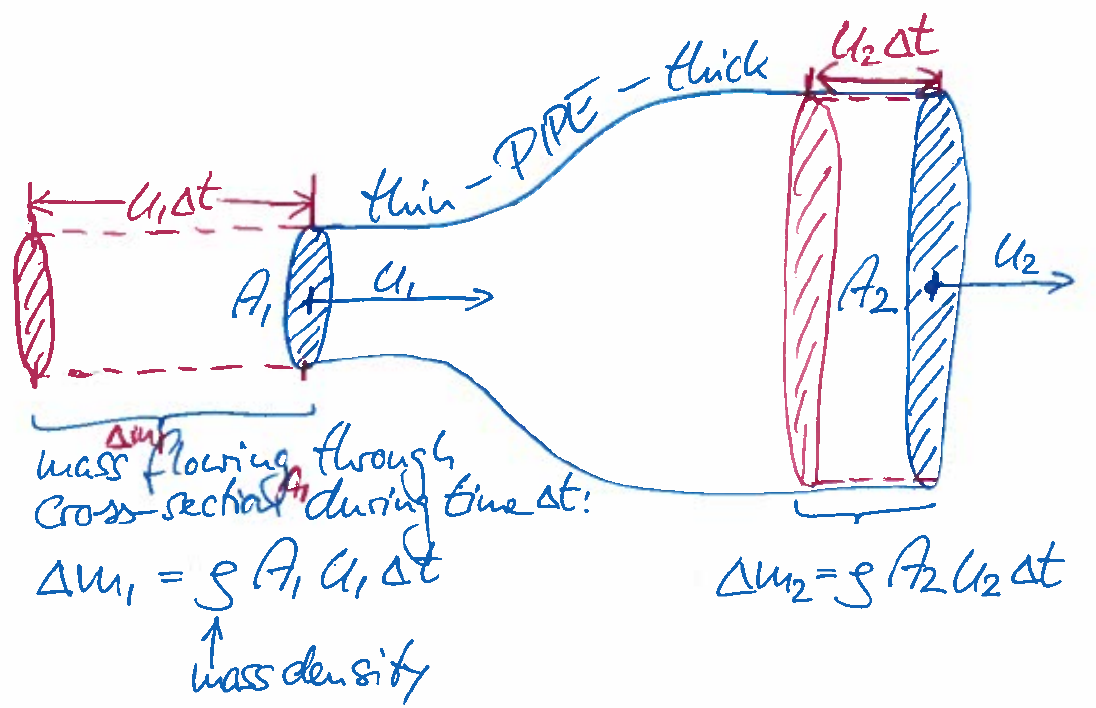
\includegraphics[width=.7\textwidth]{week1/leonardos-law}
    \caption{An illustration of mass conservation.}
    \label{fig:leonardos-law}
\end{figure}

Mass conservation means that the inflow on the left side must equal the outflow on the right side. That is
\begin{align}
    \Delta m_1 &= \Delta m_2\\
    &\Downarrow\notag\\
    \rho A_1 u_1 \Delta t &= \rho A_2 u_2 \Delta t\\
    &\Downarrow\notag\\
    A_1 u_1 &= A_2 u_2 \label{eq:leonardos-law}
\end{align}
Here \eqref{eq:leonardos-law} is known as Leonardo's Law. It has the following properties:
\begin{align}
    A_1 < A_ 2 &\Rightarrow u_1 > u_2\\
    A_1 > A_ 2 &\Rightarrow u_1 < u_2.
    \label{}
\end{align}

\subsubsection{Example 1: why is it always windy on Aarhus Ø?}
\begin{figure}[!h]
    \centering
    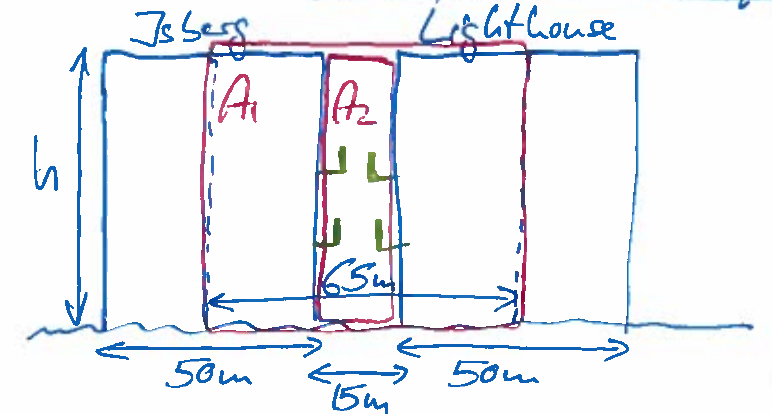
\includegraphics[width=.6\textwidth]{week1/aarhus-oe}
    \caption{The gap between adjacent apartment buildings seen from the side.}
    \label{fig:aarhus-oe}
\end{figure}

In front of the houses:
\begin{equation}
    \Delta m_1 = \rho_\mathrm{air} A_1 u_1 \Delta t
    \label{eq:aarhus-1}
\end{equation}
Between the two houses:
\begin{equation}
    \Delta m_2 = \rho_\mathrm{air} A_2 u_2 \Delta t
    \label{eq:aarhus-2}
\end{equation}
Equating \eqref{eq:aarhus-1} and \eqref{eq:aarhus-2} gives
\begin{equation}
    u_2 = \frac{A_1}{A_2} u_1
    \label{}
\end{equation}
Plugging in "realistic" numbers:
\begin{equation}
    u_2 = \frac{\SI{65}{m}\cdot\mathrm{h}}{\SI{15}{m}\cdot\mathrm{h}} \cdot \SI{10}{m/s} = \SI{43.3}{m/s}
    \label{}
\end{equation}

\begin{description}
    \item[Question:] Why balconies?
    \item[Answer:] Architects are not engineers/physicists!
\end{description}


\subsubsection{Example 2: falling stream of liquid}
\begin{figure}[h!]
    \centering
    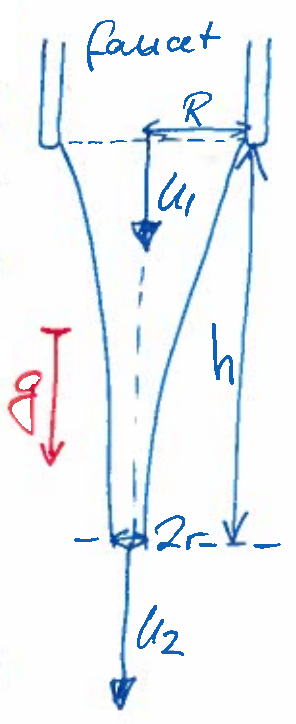
\includegraphics[width=.2\textwidth]{week1/falling-liquid}
    \caption{A stream of falling liquid.}
    \label{fig:falling-liquid}
\end{figure}

We use Leonardo's law:
\begin{equation}
    \pi R^2 u_1 = \pi r^2 u_2
    \label{}
\end{equation}
Energy conservation tells us that the sum of kinetic and potential energy is conserved:
\begin{align}
    \frac{m}{2}u_2^2 &= \frac{m}{2}u_1^2 + mgh\\
    &\Downarrow\notag\\
    u_2^2 &= u_1^2 + 2gh,
    \label{}
\end{align}
where $g=\SI{9.82}{m/S^2}$ is the acceleration of gravity.

\begin{align}
    \frac{r}{R} &= \left(\frac{\pi r^2}{\pi R^2}\right)^\frac{1}{2} = \left(\frac{A_2}{A_1}\right)^\frac{1}{2} = \left(\frac{u_1}{u_2}\right)^\frac{1}{2}\\
    &= \left(\frac{u_1^2}{u_2^2}\right)^\frac{1}{4} = \left(\frac{u_1^2}{u_1^2+2gh}\right)^\frac{1}{4}
    \label{}
\end{align}

\begin{framed}
Remark: The narrowing of a falling stream of liquid holds only for the upper part of the stream. At some height $h$ the stream becomes too thin and drop formation sets in.
\end{framed}


\subsubsection{Example 3: wave energy converter}
\begin{figure}[h!]
    \centering
    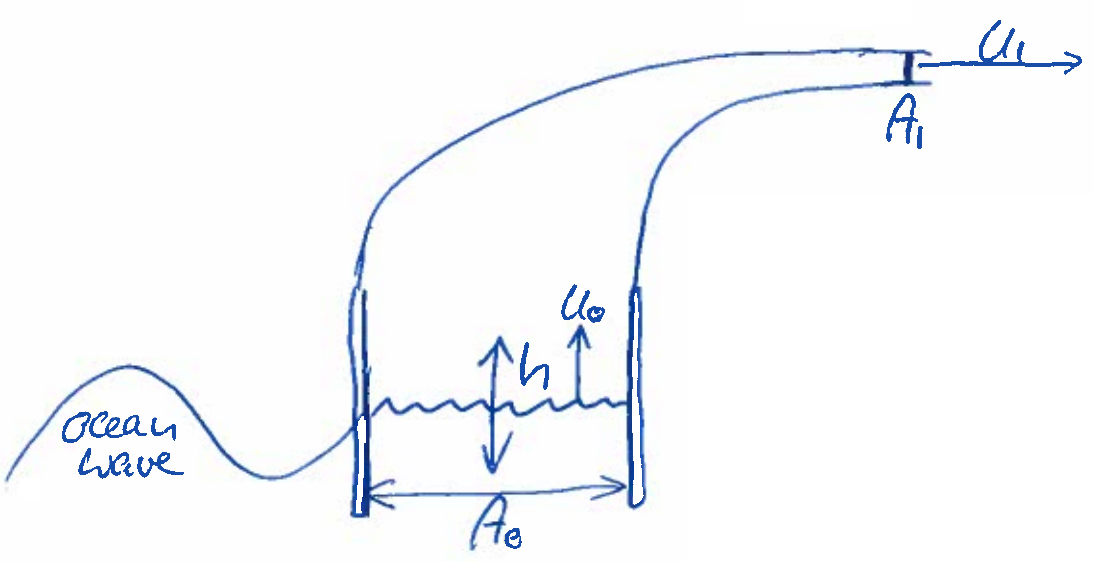
\includegraphics[width=.7\textwidth]{week1/wave-energy}
    \caption{Schematic of a wave energy converter.}
    \label{fig:wave-energy}
\end{figure}
The ocean waves induce an oscillating water surface height, which induces an oscillating air stream. A turbine is placed at the nozzle (with cross-section $A_1\ll A_0$) and extracts power from the moving air stream.

Oscillating height:
\begin{equation}
    h(t) = H \sin \omega t, \qquad \omega = 2\pi f = \frac{2\pi}{T},
    \label{}
\end{equation}
where $f$ is the frequency, $T$ is the oscillating period and $\omega$ is the angular frequency.

\begin{align}
    u_0(t) &= \frac{dh(t)}{dt}\\
    &= H\omega \cos \omega t
    \label{}
\end{align}

\begin{align}
    A_0 u_0(t) &= A_1u_1(t)\\
    &\Downarrow\notag\\
    u_1(t) &= \frac{A_0}{A_1}u_0 \cos \omega t
    \label{}
\end{align}

\begin{equation}
    A_1 \ll A_0 \Rightarrow u_1(t) \gg u_0(t)
    \label{}
\end{equation}


\subsubsection{Example 4: wake flow behind a wind turbine and wind farm optimization}
\begin{figure}[h!]
    \centering
    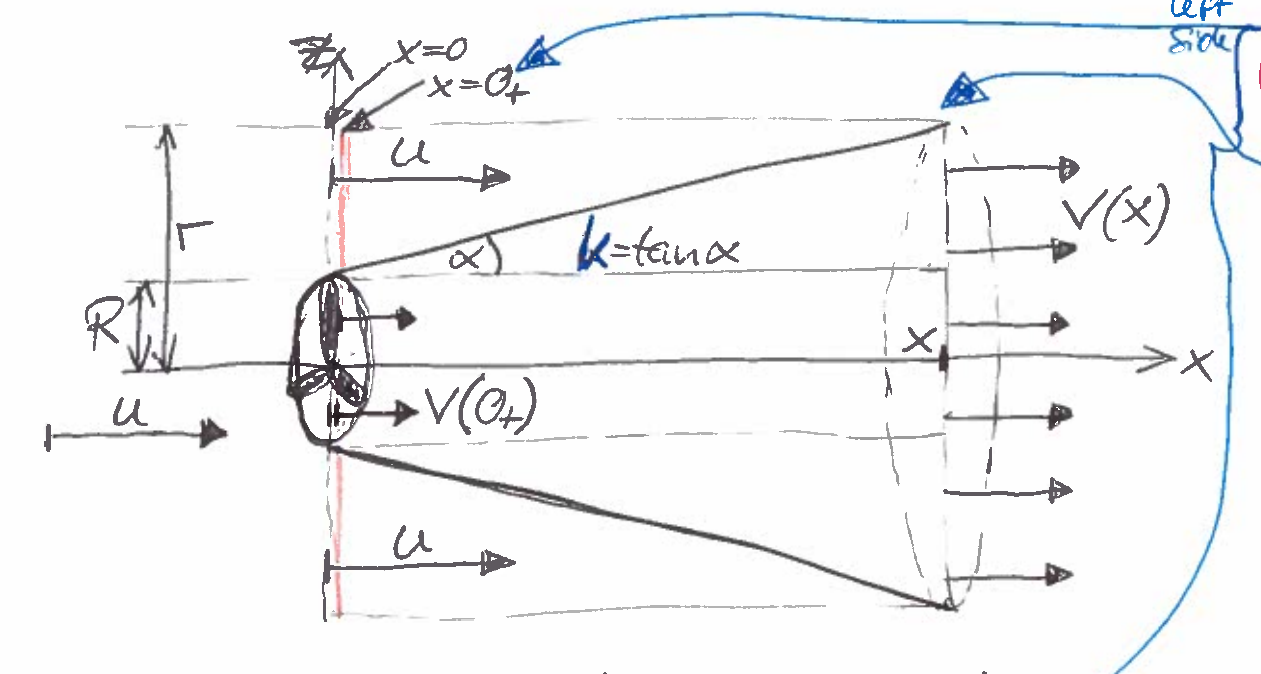
\includegraphics[width=.75\textwidth]{week1/wake-flow}
    \caption{The expanding wake behind a turbine.}
    \label{fig:wake-flow}
\end{figure}
Far-field modeling of a wake flow behind a wind turbine. We use the linear wake expansion:
\begin{equation}
    r = R + kx.
    \label{}
\end{equation}
We use the equation of continuity (Leonardo's law):
\begin{equation}
    \frac{\Delta m}{\Delta t}\biggm\vert_{x=0^+} = \rho\pi R^2v(0^+) + \rho\pi(r^2-R^2)u = \rho\pi r^2 v(x) = \frac{\Delta m}{\Delta t}\biggm\vert_x.
    \label{}
\end{equation}
In words this equation states that the in-flow through the left side of the cylinder is equal to the out-flow through the right side of the cylinder. Rearranging this equation we can get an expression for the wind speed of the wake behind the turbine:
\begin{align}
    v(x) &= \frac{R^2}{r^2}v(0_+)+\frac{r^2-R^2}{r^2}u = u-\frac{R^2}{r^2}\left(u-v(0_+)\right)\\
    &= u \left\{1-\frac{1-\frac{v(0_+)}{u}}{\left(1+\frac{kx}{R}\right)^2}\right\}.
    \label{eq:v-x}
\end{align}
The ratio
\begin{equation}
    q = \frac{v(0_+)}{u}
\end{equation}
is called the axial induction factor.

Consistency checks:
\begin{align}
    \lim_{x\rightarrow 0_+} v(x) &= v(0_+)\\
    \lim_{x\rightarrow\infty} v(x) &= u
\end{align}


\subsubsection*{Betz theory: power produced by a wind turbine}
\begin{figure}[h!]
    \centering
    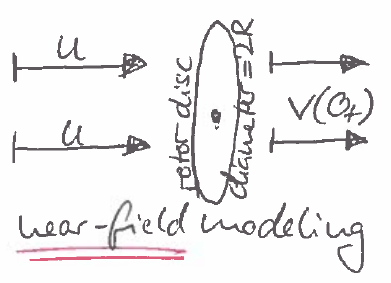
\includegraphics[width=.5\textwidth]{week1/near-field}
    \caption{The velocity deficit caused by the rotor disc.}
    \label{fig:betz}
\end{figure}

A wind turbine extracts kinetic energy out of the wind flow:
\begin{align}
    E_\mathrm{extracted} &= \frac{m}{2} \left(u^2-v^2(0_+)\right)\\
    &= \frac{1}{2}\rho\pi R^2\frac{u+v(0_+)}{2}\Delta t (u^2-v^2(0_+))
    \label{}
\end{align}

\begin{align}
    P_\mathrm{turbine} &= \frac{d E_\mathrm{extracted}}{dt}\\
    &= \frac{\rho\pi R^2 u^3}{2} \left\{\frac{\left(1+q\right)}{2}\left(1-q^2\right)\right\}
    \label{}
\end{align}
The term in front is the kinetic energy contained in the upstream wind (volume). The term within the curly brackets is the efficiency of the wind turbine also called the power coefficient:
\begin{equation}
    C_p = C_p(q) = \frac{\left(1+q\right)}{2}\left(1-q^2\right).
    \label{}
\end{equation}

The maximum efficiency of a turbine can be calculated by requiring
\begin{equation}
\diff{C_p(q)}{q} = \diff{}{q} \left(\half (1+q)(1-q^2)\right) \require 0
\label{eq:power-coefficient}
\end{equation}
This gives the optimal $q$ value
\begin{align}
q &= \frac{1}{3}\\
\leadsto
v(0_+) &= \frac{1}{3}u.
\end{align}

We can then calculate the power coefficient
\begin{equation}
\max_q C_p(q) = C_p(q=\frac{1}{3}) = \frac{16}{27} \approx 0.59.
\end{equation}
This is known as the Betz limit. Real turbines have about $C_p \approx 0.40-0.50$.


\subsubsection{Power optimization of a two-turbine wind farm}
\begin{figure}[h!]
    \centering
    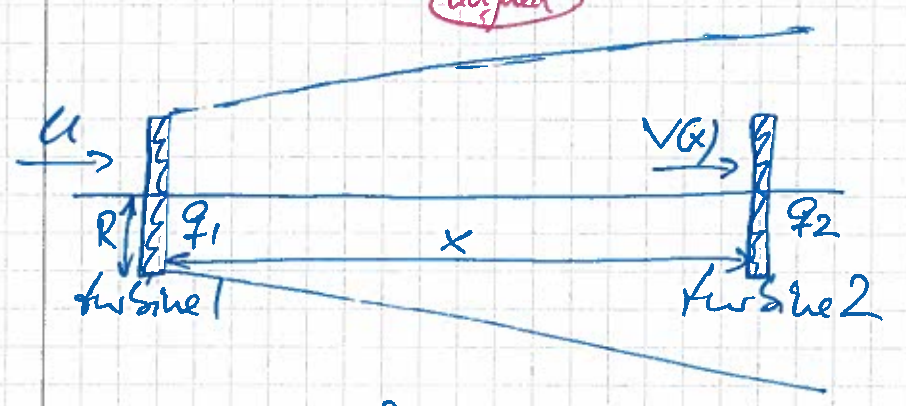
\includegraphics[width=.6\textwidth]{week1/two-turbines}
    \caption{A very simple wind farm consisting of two turbines. The wind is approaching from the left.}
    \label{fig:two-turbines}
\end{figure}

We look at a wind farm with two turbines and a wind direction aligned along the connecting line. The total output of the two turbines is
\begin{equation}
P_{1+2} = \frac{\rho\pi R^2}{2}C_{p_1}(q_1)u^3 + \frac{\rho\pi R^2}{2}C_{p_2}(q_2)v^3(x)
\end{equation}

There are no turbines behind turbine 2, so we configure it to extract the maximum amount of energy from the wind
\begin{equation}
q_2=\frac{1}{3} \Rightarrow C_{p_2}(q_2) = \frac{16}{27}
\end{equation}

Using previous expressions for $C_p(q)$ \eqref{eq:power-coefficient} and $v(x)$ \eqref{eq:v-x} the total output of the two turbines is
\begin{equation}
P_{1+2} = \frac{\rho\pi R^2}{2}u^3 \left\{\half(1+q_1)(1-q_1^2) + \frac{16}{27}\left[1-\frac{1-q_1}{\left(1+\frac{kx}{R}\right)} \right]^3 \right\}
\end{equation}

Similar to before we find the optimal value of $q_1$ by the requirement
\begin{equation}
\diff{P_{1+2}}{q_1} \require 0.
\end{equation}
We fix the values
\begin{align*}
k &= 0.04\\
\frac{x}{R} &= 8.
\end{align*}
The optimal $q$-value for turbine 1 is then
\begin{equation}
q_1 = 0.58 > \frac{1}{3},
\end{equation}
so turbine 1 let's through more wind.

Comparing this result with a $q$-value of $\frac{1}{3}$ gives
\begin{equation}
P_{1+2}(q_1=0.58) = 1.07 \cdot P_{1+2}\left(q_1=\frac{1}{3}\right),
\end{equation}
which is a $7\%$ gain.
\section{Derivation of Navier-Stokes equation (8-20)}
The goal of this section is to find an equation, which describes the spatio-temporal evolution of the velocity field $\vec{u}(\vec{r},t)$. This is the Navier-Stokes equation, which is the most fundamental equation in Fluid Dynamics.
\begin{figure}[!h]
    \centering
    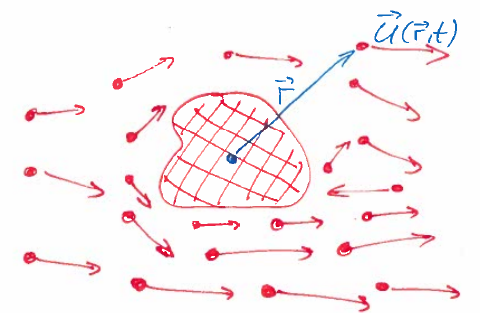
\includegraphics[width=.4\textwidth]{week2/velocity-field}
    \caption{}
    \label{fig:velocity-field}
\end{figure}

We want to describe the motion of a fluid particle. We start with Newton's second law of Classical Mechanics
\begin{equation}
\vec{F} = \diff{}{t}\left(m\vec{u}\right).
\end{equation}
The equation states that the forces acting on the particle equals its change (the time derivative) of momentum (the parenthesis).
\begin{framed}
\textbf{Remark:} in Fluid Dynamics we look not only at one fluid particle, but at all fluid particles.
\end{framed}
\begin{equation}
\diff{}{t}\left(m\vec{u}\right) = \diff{m}{t}\vec{u}+m\diff{\vec{u}}{t}=\rho\Delta V\diff{\vec{u}}{t}.
\end{equation}
The mass of a fluid particle is constant and does not change over time, hence the time derivative term is zero. We also used the relation
\begin{equation}
m=\rho\Delta V.
\end{equation}
Given the field description $\vec{u}=\vec{u}(\vec{r},t)$, we have to be a little careful with $\diff{\vec{u}}{t}$. The following is wrong:
\begin{equation}
\diff{\vec{u}}{t} = \diff{\vec{u}(\vec{r},t)}{t} = \lim_{\Delta t \rightarrow 0} \frac{\vec{u}(\vec{r},t+\Delta t) - \vec{u}(\vec{r},t)}{\Delta t}
\end{equation}
See the example in \fref{fig:fluid-particles}.

\begin{figure}[!h]
    \centering
    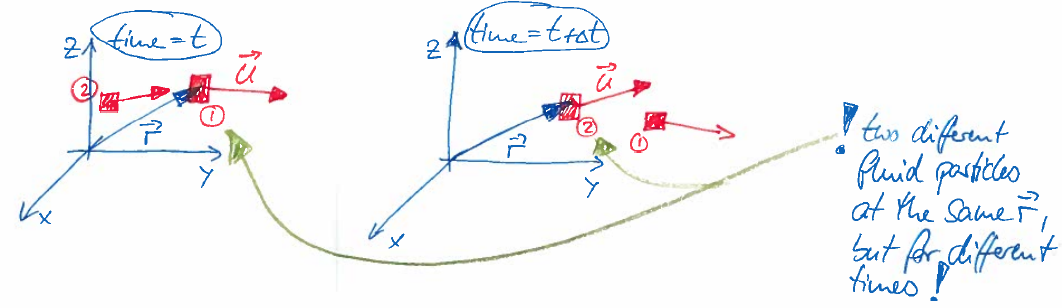
\includegraphics[width=.8\textwidth]{week2/fluid-particles}
    \caption{}
    \label{fig:fluid-particles}
\end{figure}

The correct approach is to follow one fluid particle on its pathline (trajectory) $\vec{r}=\vec{r}(\vec{r}_0,t_0;t)$. See \fref{fig:fluid-particle}.
\begin{figure}[!h]
    \centering
    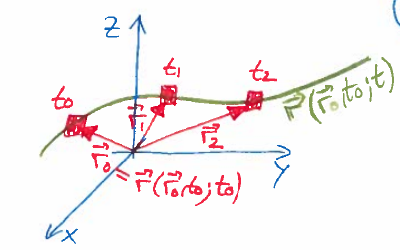
\includegraphics[width=.4\textwidth]{week2/fluid-particle}
    \caption{}
    \label{fig:fluid-particle}
\end{figure}

\begin{align}
\diff{\vec{u}}{t} &= \diff{\vec{u}\left(\vec{r}\left(\vec{r}_1,t_0;t\right),t\right)}{t}\\
&=\diff{\vec{u}(x(\vec{r}_0,t_0;t),y(\vec{r}_0,t_0;t),z(\vec{r}_0,t_0;t))}{t}\\
&=\pdiff{\vec{u}}{x}\diff{x}{t} + \pdiff{\vec{u}}{y}\diff{y}{t} + \pdiff{\vec{u}}{z}\diff{z}{t} + \pdiff{\vec{u}}{t}\diff{t}{t}\\
&= \left(u_x\pdiff{}{x} + u_y\pdiff{}{y} + u_z\pdiff{}{z}\right)\vec{u}+\pdiff{\vec{u}}{t}
\end{align}
\fxnote{should we include the calculus here or make an appendix?}
The terms in parentheses is the definition of divergence giving the final expression
\begin{equation}
\diff{\vec{u}}{t} = \pdiff{\vec{u}}{t} + \left(\vec{u}\cdot\vec{\nabla}\right)\vec{u}.
\end{equation}

\begin{framed}
The material derivative is defined as
\begin{equation}
\diff{}{t}\partial_t+\vec{u}\cdot\vec{\nabla}=\frac{D}{Dt}=D_t.
\end{equation}
Whenever we have the time derivative of a field, like $\vec{u}(\vec{r},t)$, then we have to "go with the fluid particle" and use the material derivative.
\end{framed}
We now go back to Newton's second equation:
\begin{equation}
\diff{}{t}(m\vec{u}) = \rho\Delta V\left(\partial_t + \vec{u}\cdot\vec{\nabla}\right)\vec{u} = \vec{F} = \vec{F}_\mathrm{external} + \vec{F}_\mathrm{surrounding}
\end{equation}
\fxnote{include the external force example?}
The surrounding force can be decomposed into
\begin{equation}
\vec{F}_\mathrm{surrounding} = \vec{F}_\mathrm{pressure} + \vec{F}_\mathrm{friction}
\end{equation}
The surrounding fluid particles push the "sandwiched" fluid particle around; they exert pressure. Mutual friction between neighboring fluid particles due to relative and rotational motion, deformation and compression.


\subsection{Pressure force}
\begin{figure}[!h]
    \centering
    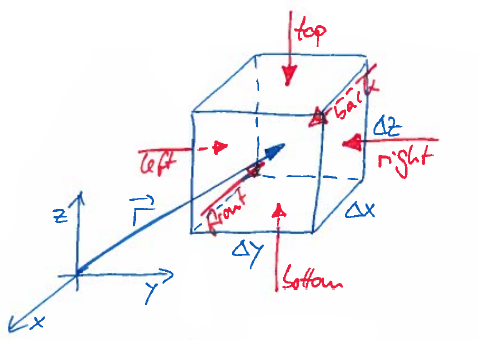
\includegraphics[width=.4\textwidth]{week2/pressure-force}
    \caption{}
    \label{fig:pressure-force}
\end{figure}

\begin{align}
\left(\vec{F}_\mathrm{pressure}\right)_z &= \vec{F}_\mathrm{pressure}^\mathrm{top} + \vec{F}_\mathrm{pressure}^\mathrm{bottom}\\
&= -p\left(x,y,z+\frac{\Delta z}{2}\right)\Delta x \Delta y + p\left(x,y,z-\frac{\Delta z}{2}\right)\Delta x \Delta y \\
\begin{split}&= -\left(p(x,y,z)+\pdiff{p(x,y,z)}{z}\frac{\Delta z}{2}\right)\Delta x \Delta y\\
&\hspace{4.5mm}+ \left(p(x,y,z)+\pdiff{p(x,y,z)}{z}\left(-\frac{\Delta z}{2}\right)\right)\Delta x \Delta y
\end{split}\\
&= -\pdiff{p(x,y,z)}{z} \Delta x \Delta y \Delta z
\end{align}
Using $\Delta x \Delta y \Delta z = \Delta V$ the pressure force density is
\begin{equation}
f_\mathrm{pressure} = \frac{\vec{F}_\mathrm{pressure}}{\Delta V} = -\vec{\nabla}p(\vec{r},t)
\end{equation}


\subsection{Friction force}
\begin{figure}[!h]
    \centering
    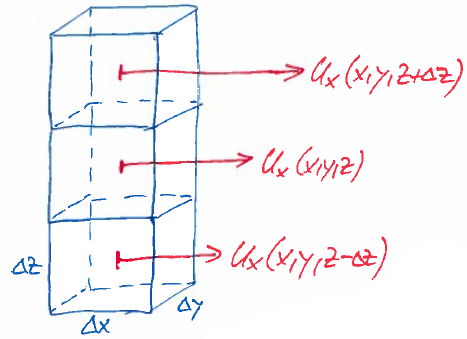
\includegraphics[width=.4\textwidth]{week2/friction-force}
    \caption{}
    \label{fig:friction-force}
\end{figure}

We consider the neighboring fluid particles above and below as sketched in \fref{fig:friction-force}.

\begin{equation}
\begin{split}
\left(\vec{F}_\mathrm{friction}^\mathrm{top+bottom}\right)_x &= \frac{\mu}{\Delta z}\Delta x \Delta y \left(U_x(x,y,z+\Delta z)-u_x(x,y,z)\right) \\
&\hspace{4.5mm}+ \frac{\mu}{\Delta z}\Delta x \Delta y \left(U_x(x,y,z-\Delta z)-u_x(x,y,z)\right)
\end{split}
\end{equation}

If $u_x(x,y,z+\Delta z)>u_x(x,y,z)$, then the fluid particle above pulls the sandwiched fluid particle with it.

Taylor series expansion and keep up to second order terms
\begin{align}
\begin{split}
\left(\vec{F}_\mathrm{friction}^\mathrm{top+bottom}\right)_x &= \frac{\mu\Delta x  \Delta y}{\Delta z}
\left\{u_x(x,y,z)+\pdiff{u_x(x,y,z)}{z}\Delta z + \ppdiff{u_x(x,y,z)}{z}\frac{\Delta z^2}{2} + \cdots \right.\\
&\hspace{4.5mm} - u_x(x,y,z) + u_x(x,y,z)+\pdiff{u_x(x,y,z)}{z}(-\Delta z) \\
&\hspace{4.5mm} + \left. \ppdiff{u_x(x,y,z)}{z}\frac{(-\Delta z)^2}{2} + \cdots - u_x(x,y,z) \right\}
\end{split}\\
&= \mu \Delta x \Delta y \Delta z \ppdiff{u_x(x,y,z)}{z}
\end{align}

front + back:
\begin{equation}
\left(\vec{F}_\mathrm{friction}^\mathrm{front+back}\right)_x = \mu\Delta V \ppdiff{u_x(x,y,z)}{y}
\end{equation}

Most general expression of the friction force:
\begin{equation}
\frac{\vec{F}_\mathrm{friction}}{\Delta V} = \vec{f}_\mathrm{friction} \left(\pdiff{^2u_i}{x_k\partial x_l}\right) = \vec{f}_\mathrm{friction} (\vec{\nabla},\vec{\nabla},\vec{u})
\end{equation}

The task is to build a vector $\vec{f}$ from a combination of three vectors $\vec{a}=\vec{\nabla}, \vec{b}=\vec{\nabla}, \vec{c}=\vec{u}$, such that
\begin{equation}
\vec{f} = \alpha\left(\vec{a}\cdot\vec{b}\right)\vec{c} + \beta\left(\vec{a}\cdot\vec{c}\right)\vec{b} + \alpha \left(\vec{b}\cdot\vec{c}\right)\vec{a}
\end{equation}

The solution:
\begin{equation}
\vec{f}_\mathrm{friction} = \mu\left(\vec{\nabla}\cdot\vec{\nabla}\right)\vec{u} + \left(\mu_v+\frac{\mu}{3}\right)\vec{\nabla}\left(\vec{\nabla}\cdot\vec{u}\right),
\end{equation}
where $\mu$ is the shear (dynamic) viscosity and $\mu_v$ is the compression (bulk) viscosity.

Navier-Stokes equation:
\begin{equation}
\rho\left(\partial_t+\left(\vec{u}\cdot\vec{\nabla}\right)\right)\vec{u} = \vec{f}\mathrm{ext}-\vec{\nabla}p + \mu\left(\vec{\nabla}\cdot\vec{\nabla}\right)\vec{u} + \left(\mu_v+\frac{\mu}{3}\right)\vec{\nabla}\left(\vec{\nabla}\cdot\vec{u}\right)
\end{equation}
where
\begin{align}
\vec{u} &= \vec{u}\left(\vec{r},t\right)\\
p &= p\left(\vec{r},t\right)\\
\rho &= \rho\left(\vec{r},t\right)\\
\vec{f}_\mathrm{ext} &= \vec{f}_\mathrm{ext}\left(\vec{r},t\right)
\end{align}


\subsection{Navier-Stokes equation in components}
\begin{align}
\begin{split}\rho
\begin{pmatrix}
\pdiff{u_x}{t} \\ \pdiff{u_y}{t} \\ \pdiff{u_z}{t}
\end{pmatrix} +
\rho
\begin{pmatrix}
\left(u_x\pdiff{}{x}+u_y\pdiff{}{y}+u_z\pdiff{}{z}\right)u_x \\
\left(u_x\pdiff{}{x}+u_y\pdiff{}{y}+u_z\pdiff{}{z}\right)u_y \\
\left(u_x\pdiff{}{x}+u_y\pdiff{}{y}+u_z\pdiff{}{z}\right)u_z
\end{pmatrix} &= 
\begin{pmatrix}
f_x^\mathrm{ext} \\ f_y^\mathrm{ext} \\ f_z^\mathrm{ext}
\end{pmatrix} -
\begin{pmatrix}
\pdiff{p}{x} \\ \pdiff{p}{y} \\ \pdiff{p}{z}
\end{pmatrix} \\
&\hspace{4.5mm}+
\mu
\begin{pmatrix}
\left(\ppdiff{}{x}+\ppdiff{}{y}+\ppdiff{}{z}\right)u_x \\
\left(\ppdiff{}{x}+\ppdiff{}{y}+\ppdiff{}{z}\right)u_y \\
\left(\ppdiff{}{x}+\ppdiff{}{y}+\ppdiff{}{z}\right)u_z
\end{pmatrix} \\
&\hspace{4.5mm}+
\left(\mu_v + \frac{\mu}{3}\right) +
\begin{pmatrix}
\pdiff{}{x}\left(\pdiff{}{x}+\pdiff{}{y}+\pdiff{}{z}\right) \\
\pdiff{}{y}\left(\pdiff{}{x}+\pdiff{}{y}+\pdiff{}{z}\right) \\
\pdiff{}{z}\left(\pdiff{}{x}+\pdiff{}{y}+\pdiff{}{z}\right)
\end{pmatrix}
\end{split}
\end{align}

\begin{framed}
\textbf{Remark:} There are only a few exact analytical solutions; many approximate analytical solutions (guided by intuition). Computational fluid dynamics can give us "exact" numerical solutions for approximations to the Navier-Stokes equation.
\end{framed}

We now have three coupled differential equations for five fields: $u_x\left(\vec{r},t\right)$, $u_y\left(\vec{r},t\right)$, $u_z\left(\vec{r},t\right)$, $p\left(\vec{r},t\right)$, and $\rho\left(\vec{r},t\right)$. This means we are missing two differential equations.


\subsection*{The first missing equation}
From thermodynamics we have an equation of state
\begin{equation}
g(p,\rho)=0
\end{equation}

Incompressible flow
\begin{equation}
\rho = \mathrm{constant}
\end{equation}

Law of ideal gases
\begin{equation}
pV=NkT
\end{equation}

From these we get
\begin{align}
\rho &= \frac{N}{V} = \frac{1}{kT}p\\
\frac{p}{\rho} &= kT = \mathrm{constant}
\end{align}
This only holds if the temperature is constant.


\subsection*{The second missing equation}
Equation of continuity, local mass conservation.

\begin{figure}[!h]
    \centering
    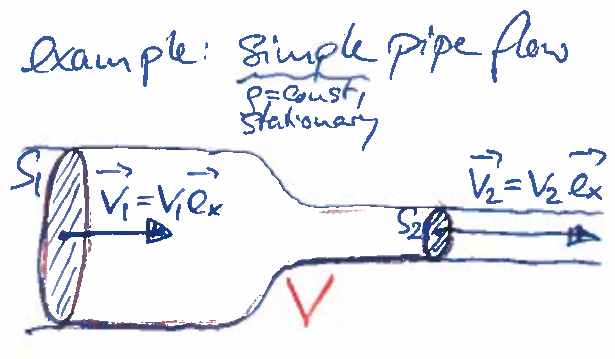
\includegraphics[width=.4\textwidth]{week2/pipe-flow}
    \caption{}
    \label{fig:pipe-flow}
\end{figure}

\begin{framed}
\textbf{Example:} simple pipe flow. See \fref{fig:pipe-flow}.

\begin{align}
M_\mathrm{in} &= \rho S_1v_1\Delta t \\
M_\mathrm{out} &= \rho S_2v_2\Delta t
\end{align}

mass conservation
\begin{align}
M_\mathrm{in} &= M_\mathrm{out}\\
\leadsto
v_1S_1 &= v_2S_2
\end{align}
This is Leonardo's law.
\end{framed}

Local mass conservation in a small volume element:
\begin{figure}[!h]
    \centering
    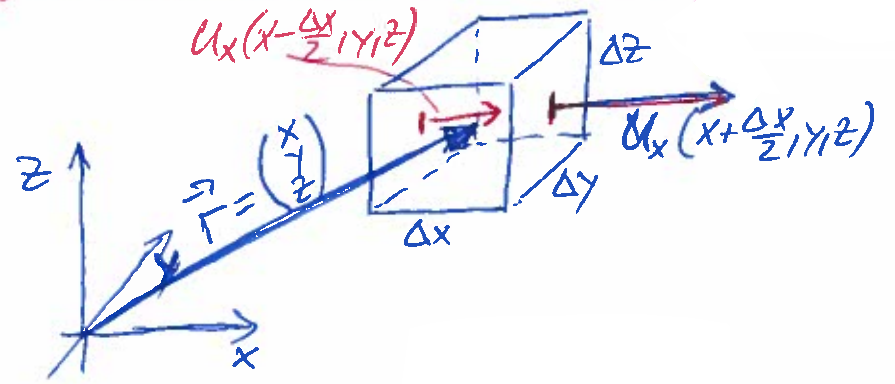
\includegraphics[width=.5\textwidth]{week2/mass-conservation}
    \caption{}
    \label{fig:mass-conservation}
\end{figure}

Mass flux through surface of volume $\Delta V = \Delta x \Delta y \Delta z$ in $x$-direction:
\begin{align}
\begin{split}
\diff{M_x^S}{t} &= \rho \left(x+\frac{\Delta x}{2},y,z,t\right)u_x\left(x+\frac{\Delta x}{2},y,z,t\right)\Delta y \Delta z\\
&\hspace{4.5mm} - \rho \left(x+\frac{\Delta x}{2},y,z\right)u_x\left(x+\frac{\Delta x}{2},y,z\right)\Delta y \Delta z
\\
&=\left(\rho(x,,z)+\pdiff{\rho(x,y,z)}{x}\frac{\Delta x}{2}\right)\left(u_x(x,y,z)+\pdiff{u_x(x,y,z)}{x}\frac{\Delta x}{2}\right) \Delta y \Delta z \\
&\hspace{4.5mm} - \left[\rho(x,,z)+\pdiff{\rho(x,y,z)}{x}\left(-\frac{\Delta x}{2}\right)\right]\left[u_x(x,y,z)+\pdiff{u_x(x,y,z)}{x}\left(-\frac{\Delta x}{2}\right)\right] \Delta y \Delta z
\\
&=\pdiff{\rho(x,y,z)}{x}u_x(x,y,z)\Delta x \Delta y \Delta z  + \rho(x,y,z)\pdiff{u_x(x,y,z)}{x}\Delta x \Delta y \Delta z\\
&=\pdiff{\left(\rho(x,y,z,t)u_x(x,y,z,t)\right)}{x}\Delta V
\end{split}
\end{align}

Mass flux in $y$ and $z$-direction:
\begin{align}
\diff{M_y^S}{t} &= \pdiff{(\rho(x,y,z)u_y(x,y,z))}{y}\Delta V\\
\diff{M_z^S}{t} &= \pdiff{(\rho(x,y,z)u_z(x,y,z))}{z}\Delta V
\end{align}

Sum of mass fluxes through volume in all directions:
\begin{align}
\diff{M^S}{t} &= \diff{M_x^S}{t} + \diff{M_y^S}{t} + \diff{M_z^S}{t} \\
&= \pdiff{(\rho u_x)}{x}\Delta V + \pdiff{(\rho u_y)}{y}\Delta V + \pdiff{(\rho u_z)}{z}\Delta V\\
&=
\begin{pmatrix}
\pdiff{}{x} \\ \pdiff{}{y} \\ \pdiff{}{z} \cdot
\end{pmatrix}
\begin{pmatrix}
\rho u_x \\ \rho u_y \\ \rho u_z
\end{pmatrix}
\Delta V \\
&= \vec{\nabla}\cdot\left(\rho(x,y,z)\vec{u}(x,y,z)\right)\Delta V
\end{align}

Increase of mass within fixed volume $\Delta V$:
\begin{equation}
\diff{M^V}{t} = \diff{(\rho(\vec{r},t)\Delta V)}{t} = \pdiff{\rho(\vec{r},t)}{t}\Delta V
\end{equation}

Local mass conservation
\begin{equation}
\diff{M^V}{t} = -\diff{M^S}{t}
\end{equation}
If mass within the volume increases, then less has to flow out of the surface than to flow in
\begin{equation}
\pdiff{\rho(\vec{r},t)}{t}+\vec{\nabla}\cdot\left(\rho(\vec{r},t)\vec{u}(\vec{r},t)\right)=0
\end{equation}
This is the equation of continuity.

\begin{shaded}
Include the generalized example on page 19 of hand written notes?
\end{shaded}

\subsection{Summary}
Navier-Stokes equation:
\begin{equation}\label{eq:navier-stokes}
\rho\left(\pdiff{}{t}+\left(\vec{u}\cdot\vec{\nabla}\right)\right)\vec{u} = f_\mathrm{ext}-\vec{\nabla}p+\mu\left(\vec{\nabla}\cdot\vec{\nabla}\right)\vec{u} + \left(\mu_v + \frac{\mu}{3}\right)\vec{\nabla}\left(\vec{\nabla}\cdot\vec{u}\right)
\end{equation}

\begin{align}
\vec{u} &= \vec{u}(\vec{r},t) = \vec{u}(x,y,z,t) \\
\rho &= \rho(\vec{r},t)\\
p &= p(\vec{r},t)
\end{align}

equation of continuity:
\begin{equation}
\pdiff{\rho}{t}+\vec{\nabla}\cdot(\rho\vec{u})=0
\end{equation}

Equation of state:
\begin{equation}
g(p,\rho;T)=0
\end{equation}

Heat equation:
\begin{equation}
\left(\pdiff{}{t}+\left(\vec{u}\cdot\vec{\nabla}\right)\right)T(\vec{r},r) = \kappa\left(\vec{\nabla}\cdot\vec{\nabla}\right)T(\vec{r},t),
\end{equation}
where $\kappa$ is the thermal diffusion.

\newpage
\section{Simplification of the Navier-Stokes equation (21-25)}

\subsection{Simplification I: incompressible flows}
Incompressibility means that the density of a fluid particle (moving along its pathline) remains constant.

Incompressiblity is a very good approximation for most liquids, including water. In $\SI{1000}{m}$ depth the density of seawater is only $0.4\%$ larger that at the surface. For gas glows incompressiblity is also a good approximation as long as $|\vec{u}_\mathrm{gas}| \ll \mathrm{speed\ of\ sound}$. Compressibility becomes important when discussing e.g. sound waves.

\begin{align}
0 = \diff{\rho(\vec{r},t)}{t} &= \pdiff{\rho}{t}+\left(\vec{u}\cdot\vec{\nabla}\right)\rho\\
&= -\vec{\nabla}\left(\rho\vec{u}\right)+\left(\vec{u}\cdot\vec{\nabla}\right)\rho \\
&= -\left(\vec{u}\cdot\vec{\nabla}\right)\rho - \rho\left(\vec{\nabla}\cdot\vec{u}\right) + \left(\vec{u}\cdot\vec{\nabla}\right)\rho\\
&= -\rho\left(\vec{\nabla}\cdot\vec{u}\right)\\
&= -\rho\, \mathrm{div}\, \vec{u}
\end{align}
In the first line we used the material derivative. In the step to the second line we used continuity equation.

For incompressibility the divergence must be zero:
\begin{equation}
\vec{\nabla}\cdot\vec{u} = 0
\end{equation}

Navier-Stokes equation for incompressible flows:
\begin{equation}
\rho\left(\pdiff{\vec{u}}{t}+\left(\vec{u}\cdot\vec{\nabla}\right)\right)\vec{u} = f_\mathrm{ext}-\vec{\nabla}p+\mu\left(\vec{\nabla}\cdot\vec{\nabla}\right)\vec{u}
\end{equation}
\begin{framed}
Remark: It looks simple, but these nonlinear differential equations remain a formidable challenge to engineers, physicists and mathematicians.
\end{framed}
Equation of state in the simplest form with constant density:
\begin{equation}
p=p(\rho) \Rightarrow \rho=\rho_0=\mathrm{constant}
\end{equation}


\subsection{Simplification II: incompressible, ideal, stationary, irrotational flows}
We use the incompressibility result from earlier:
\begin{equation}
\vec{\nabla}\cdot\vec{u} = 0
\end{equation}

Ideal means no friction. To eliminate friction forces we set $\mu=0$.

Euler equation:
\begin{equation}
\rho_0\left(\pdiff{\vec{u}}{t}+\left(\vec{u}\cdot\vec{\nabla}\right)\vec{u}\right) = f_\mathrm{ext}-\vec{\nabla}p
\end{equation}

stationary:
\begin{align}
\vec{u}(\vec{r},t) &= \vec{u}(\vec{r})\\
\leadsto
\pdiff{\vec{u}}{t} &= 0
\end{align}
\begin{equation}
\rho_0\left(\vec{u}\cdot\vec{\nabla}\right)\vec{u} = f_\mathrm{ext}-\vec{\nabla}p
\end{equation}

no external forces: $f_\mathrm{ext}=0$
\begin{equation}
\rho_0\left(\vec{u}\cdot\vec{\nabla}\right)\vec{u} = -\vec{\nabla}p
\end{equation}

Assuming irrotational flow: $\vec{\nabla}\times\vec{u}=0$.
\begin{equation}
\vec{\nabla}\underbrace{\left(\frac{\rho_0}{2}\vec{u}^2+p\right)}_\mathrm{constant}=0
\end{equation}

Bernoulli's equation
\begin{align}
\frac{\rho_0}{2}\vec{u}^2+p &= \mathrm{constant}\\
\vec{\nabla}\cdot\vec{u} &= 0\\
\vec{\nabla}\times\vec{u} &= 0
\end{align}
Given all the assumptions, this set of equations is equivalent to the Navier-Stokes equation.

\begin{shaded}
I skipped page 23a and 23b. Should these be included here?
\end{shaded}


\subsection{Derivation of Bernoulli's equation}
The equation
\begin{equation}
\vec{\nabla}\left(\frac{\rho_0}{2}\vec{v}^2+p\right) = \rho_0\vec{v}\times\left(\vec{\nabla}\times\vec{v}\right)
\end{equation}
is (scalar) multiplied with $d\vec{s}\parallel\vec{v}$, where $d\vec{s}$ describes an increment of a specific streamline (here pathline since $\vec{v}(\vec{r},t) = \vec{v}(\vec{r})$).
\begin{equation}
d\vec{s}\cdot\left[\vec{v}\times\left(\vec{\nabla}\times\vec{v}\right)\right]=0
\end{equation}
Since $d\vec{s}\parallel\vec{v}$ it must be that $d\vec{s}\perp\vec{v}\times\left(\vec{\nabla}\times\vec{v}\right)$.

Subsequent path-integration along a streamline yields
\begin{align}
0 \require ...
\end{align}


\subsection{Example: Why does an airplane fly?}
\begin{figure}[!h]
    \centering
    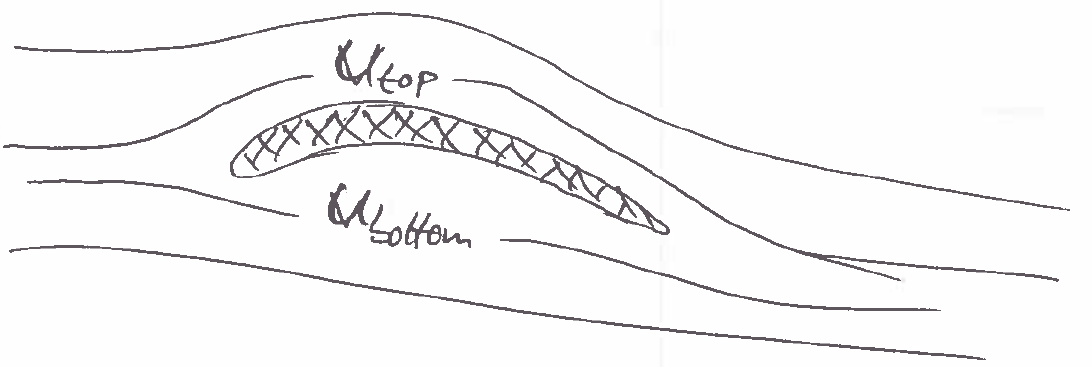
\includegraphics[width=.6\textwidth]{week2/airplane}
    \caption{}
    \label{fig:airplane}
\end{figure}
The wind speed difference between the top and bottom of the wing creates a pressure difference:
\begin{align}
u_\mathrm{top} &> u_\mathrm{bottom}\\
\leadsto
p_\mathrm{top} &< p_\mathrm{bottom}.
\end{align}
This results in a lifting force.
\section{Ideal flow: planar 2-dimensional potential flow around cylinder (26-36)}

\begin{framed}
For further details see section 4.3, 4.9 and 7.1-3 in the KCD book
\end{framed}

\begin{shaded}
I skipped the summary of NS equation on page 26 of hand written notes. Maybe there should be an introductory paragraph here with references to equations from previous sections.
\end{shaded}

\begin{figure}[!h]
    \centering
    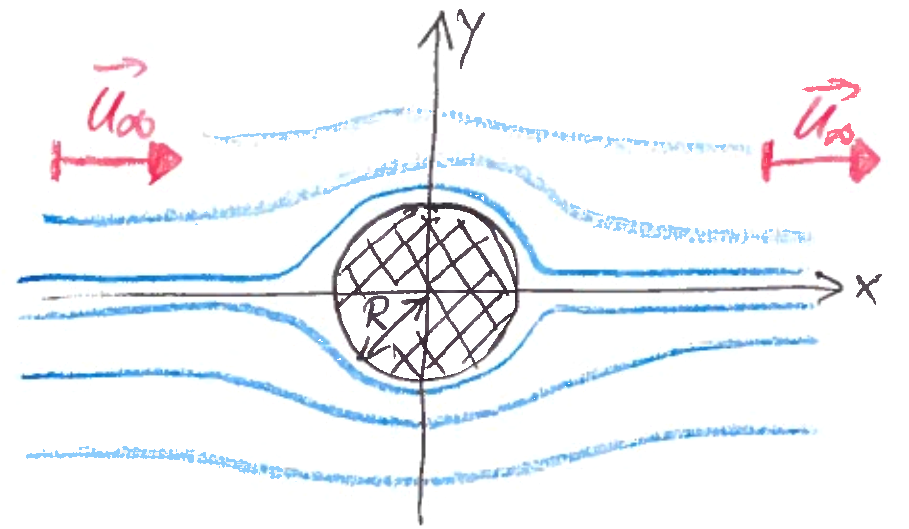
\includegraphics[width=.5\textwidth]{week3/planar-flow}
    \caption{}
    \label{fig:planar-flow}
\end{figure}

Questions to \fref{fig:planar-flow}: 1) $\vec{u} = \vec{u}(x,y,z)$?, 2) pathlines (streamlines)?

\begin{equation}
\vec{\nabla}\times\vec{u} = 0 \Rightarrow \vec{u}(\vec{r}) = \vec{\nabla}\phi(\vec{r})
\end{equation}
where $\phi(\vec{r})$ is a velocity potential.

\begin{align}
\vec{\nabla}\times\vec{u} &= 0\\
\leadsto
\vec{\nabla}\cdot\vec{\nabla}\phi(\vec{r}) &= \left(\ppdiff{}{x}+\ppdiff{}{y}+\ppdiff{}{z}\right)\phi(x,y)\\
&= \left(\ppdiff{}{x}+\ppdiff{}{y}\right)\phi(x,y) = 0
\end{align}
This second order differential equation is the Laplace equation.

Question: How does the cylinder (obstacle) enter in solving the Laplace equation?

Two boundary conditions.

1:
\begin{align}
\vec{u}(|\vec{r}|\rightarrow\infty) &= \vec{u}_\infty = u_\infty\vec{e}_x \\
\leadsto
\phi(|\vec{r}|\rightarrow\infty) &= u_\infty x + \mathrm{constant}
\end{align}

2:
\begin{equation}
0=u_\mathrm{surface}\cdot \vec{n} = \vec{\nabla}\phi\biggm\vert_\mathrm{surface}\cdot\vec{n}
\end{equation}

The fluid particle does not flow into the surface; only tangential component.

\begin{figure}[!h]
    \centering
    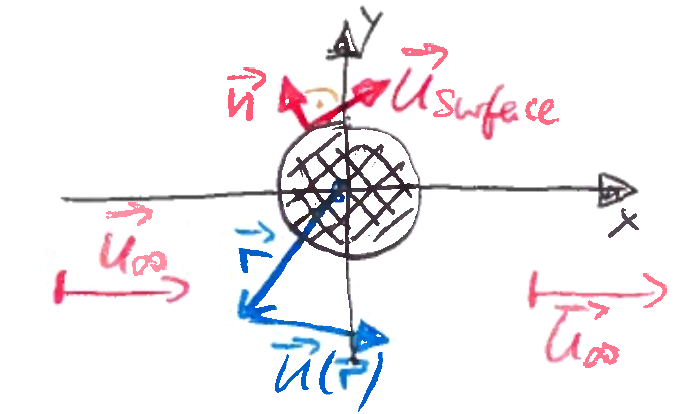
\includegraphics[width=.5\textwidth]{week3/planar-flow2}
    \caption{}
    \label{fig:planar-flow2}
\end{figure}

For the flow around the cylinder the solution of the Laplace equation with the two boundary conditions "falls from the sky" (for the moment):
\begin{equation}
\phi(x,y)=u_\infty\times\left(1+\frac{R^2}{x^2+y^2}\right)
\end{equation}

\begin{shaded}
I skipped the last part of page 28 here
\end{shaded}

Velocity field:
\begin{equation}
\vec{u} = \begin{pmatrix}
u_x\\u_y
\end{pmatrix}  = 
\vec{\nabla}\phi(x,y) = \begin{pmatrix}
\pdiff{\phi}{x} \\
\pdiff{\phi}{y}
\end{pmatrix}
\end{equation}

\begin{align}
\begin{split}\label{eq:uxuy1}
u_x &= u_\infty\left(1+\frac{R^2(y^2-x^2)}{(x^2+y^2)^2}\right)\\
u_y &= -u_\infty \frac{2xyR^2}{(x^2+y^2)^2}
\end{split}
\end{align}

\begin{figure}[!h]
    \centering
    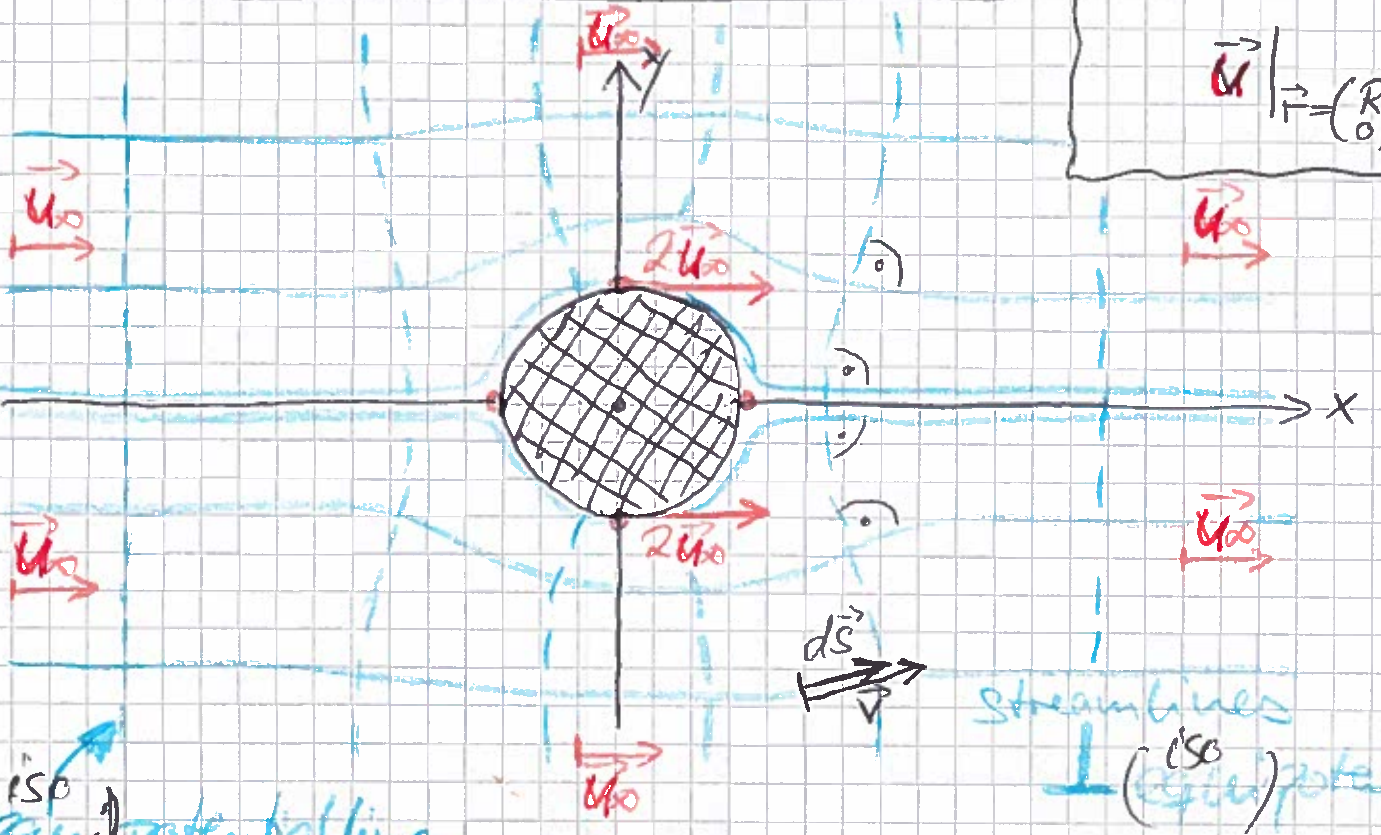
\includegraphics[width=.7\textwidth]{week3/velocity-field}
    \caption{}
    \label{fig:velocity-field}
\end{figure}

examples:
\begin{align}
\vec{u}\biggm\vert_{x\rightarrow\pm\infty} &= u_\infty\vec{e}_x = \vec{u}\biggm\vert_{y\rightarrow\pm\infty}\\
\vec{u}\biggm\vert_{\small\vec{r}=\begin{pmatrix} 0 \\ R
\end{pmatrix}} &= 2u_\infty\vec{e}_x \\
\vec{u}\biggm\vert_{\small\vec{r}=\begin{pmatrix} R \\ 0
\end{pmatrix}} &= 0 = \vec{u}\biggm\vert_{\small\vec{r}=\begin{pmatrix} -R \\ 0
\end{pmatrix}}
\end{align}


\newpage
\subsection{Pathline around a cylinder}

\begin{figure}[!h]
    \centering
    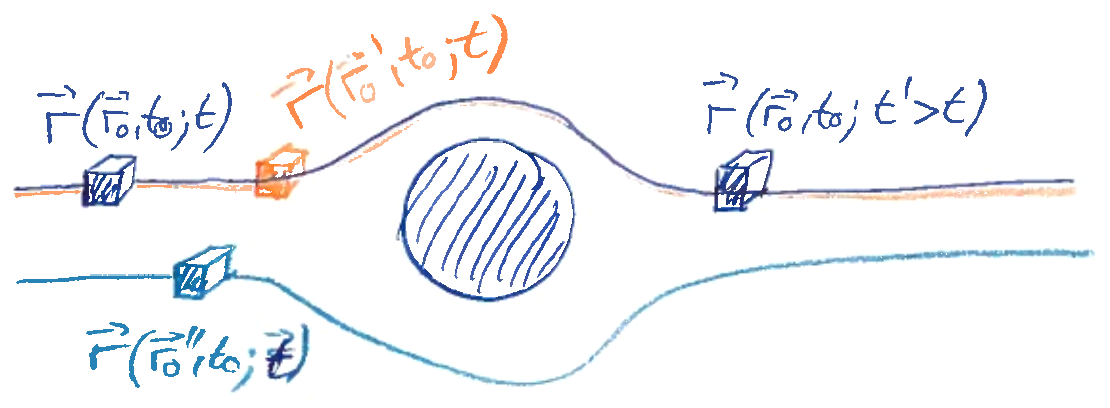
\includegraphics[width=.7\textwidth]{week3/pathline-cylinder}\\
    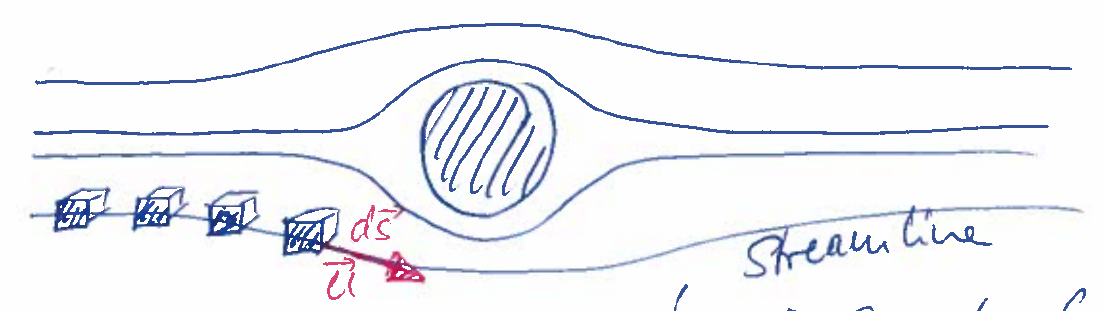
\includegraphics[width=.7\textwidth]{week3/pathline-cylinder2}
    \caption{}
    \label{fig:pathline-cylinder}
\end{figure}

Top part of \fref{fig:pathline-cylinder} shows the Lagrangian picture: follows particle through all times. the bottom part shows the Eulerian picture, which is a snapshot of all fluid particles at one particular time.

Connection between Lagrangian and Eulerian picture:
\begin{equation}
\diff{\vec{r}}{t} = \vec{u}(\vec{r},t)
\end{equation}

For stationary flows
\begin{equation}
\vec{u}(\vec{r},t)=\vec{u}(\vec{r}) \Rightarrow \mathrm{pathline} = \mathrm{streamline}
\end{equation}

Given the snapshots $\vec{u}(\vec{r},t)$, we can calculate the pathlines.

Given the pathlines, we can construct the snapshots.

This sounds like the "chicken and egg" problem.

\bigskip
Question: How to calculate the streamlines?

First approach:
Definition of streamline:
\begin{equation}
d\vec{s}\parallel\vec{u},
\end{equation}
where $ds$ is a line element of a streamline.
\begin{align}
0=d\vec{s}\times\vec{u} &=
\begin{vmatrix}
0 & 0 & \vec{e}_z \\
dx & dy & 0 \\
u_x & u_y & 0
\end{vmatrix} =
(u_ydx-u_xdy)\vec{e}_z\\
\leadsto
\diff{y}{x} &= \frac{u_y}{u_x} = -\frac{2xyR^2}{(x^2+y^2)^2+R^2(y^2-x^2)}
\end{align}

Second approach: introduce the streamfunction $\psi(x,y)$.

Incompressibility gives us:
\begin{equation}
 \vec{\nabla}\cdot\vec{u} = \pdiff{u_x}{x}+\pdiff{u_y}{y}=0
\end{equation}
which leads to
\begin{equation}
 u_x = \pdiff{\psi}{y}, \quad u_y = -\pdiff{\psi}{x} \label{eq:uxuy2}
\end{equation}

\begin{align}
d\vec{s}\times\vec{u} &= (u_ydx-u_xdy)\vec{e}_x \\
&= \left(-\pdiff{\psi}{x}dx-\pdiff{\psi}{y}dy\right)\vec{e}_z\\
&= -d\psi \vec{e}_z \require 0
\end{align}
The streamfunction is constant along a streamline. This represents an \emph{isopotentialline} of the streamfunction and describes a streamline.

From the defining functions of the streamfunction in \eqref{eq:uxuy2} and the $u_x$, $u_y$ solution for the ideal flow around a cylinder in \eqref{eq:uxuy1}, we can determine $\psi$ by partial integration
\begin{align}
\psi(x,y) &= v_\infty y\left(1-\frac{R"2}{x^2+y^2}\right)\\
&= v_\infty \sin\psi\left(r-\frac{R^2}{r}\right)
\end{align}

\begin{framed}
\textbf{Remark:} relationship between velocity potential and streamfunction $\phi=\mathrm{constant}$, $\psi=\mathrm{constant}$ represent and orthogonal set of curves, because
\begin{equation}
\left(\vec{\nabla}\phi\right)\cdot\left(\vec{\nabla}\psi\right) = 
\begin{pmatrix}
\pdiff{\phi}{x} \\ \pdiff{\phi}{y}
\end{pmatrix} \cdot
\begin{pmatrix}
\pdiff{\psi}{x} \\ \pdiff{\psi}{y}
\end{pmatrix} = 
\begin{pmatrix}
u_x \\ u_y
\end{pmatrix}\cdot
\begin{pmatrix}
-u_y \\ u_x
\end{pmatrix} = 0
\end{equation}
\end{framed}

\begin{shaded}
I left out page 32a-32d here.
\end{shaded}

Two dimensional potential flow around an infinitely long cylinder 

Because of cylinder symmetry we can transform from  to cylindrical coordinates
\begin{align}
x &= r\cos\phi\\
y &= r\sin\phi
\end{align}

\begin{equation}
\Phi(x,y) \rightarrow \Phi(r,\phi)
\end{equation}

\begin{align}
\Delta\Phi(x,y) &= \left(\ppdiff{}{x}+\ppdiff{}{y}\right)\Phi(x,y) \\
&= \left[\frac{1}{r}\pdiff{}{r}\left(r\pdiff{}{r}\right) + \frac{1}{r^2}\pdiff{}{\phi}\right]\Phi(r,\phi)\\
&= 0\\
\leadsto
r\pdiff{}{r}\left(\pdiff{\Phi}{r}\right) &= -\ppdiff{\Phi}{\phi}
\end{align}

\begin{shaded}
I left out page 33a-33b here.
\end{shaded}

Ansatz: factorization
\begin{equation}
\Phi(r,\phi) = f(r)g(\phi)
\end{equation}

\begin{align}
\frac{1}{f\cdot g} r\pdiff{}{r}\left(r\pdiff{(f(r)g(\phi))}{r}\right) &= -\frac{1}{f\cdot g}\ppdiff{(f(r)g(\phi))}{\phi} \\
\leadsto
\frac{1}{f(r)}r\pdiff{}{r}\left(r\pdiff{f(r)}{r}\right) &= -\frac{1}{g(\phi)}\ppdiff{g(\phi)}{\phi} \require m^2
\end{align}

Left part depends only on $r$, middle part depends only on $\phi$, and right part is a constant, which does neither depend on $r$ nor $\phi$.

\begin{align}
\ppdiff{g(\phi)}{\phi} &= -m^2g(\phi)\\
\leadsto
g(\phi) = e^{im\phi} &=  \cos m\phi + i\sin m\phi
\end{align}

requirement:
\begin{align}
g(\phi) &= g(\phi+2\pi)\\
\leadsto
e^{im\phi} &= e^{im(\phi+2m)}\\
\leadsto
e^{2\pi im} &= 1
\end{align}

\begin{equation}
r\pdiff{}{r}\left(r\pdiff{}{r}f(r)\right) = m^2f(r)
\end{equation}

polynomial ansatz:
\begin{equation}
f(r) = r^\alpha
\end{equation}

\begin{align}
r\pdiff{}{r}\left(r\alpha r^{\alpha-1}\right) &= \alpha^2 r^\alpha \require m^2 r^\alpha\\
leadsto
\alpha &= \pm m
\end{align}

\begin{equation}
\Phi(r,\phi) = f(r)g(\phi) = r^{\pm m}e^{im\phi}
\end{equation}

Since the Laplace equation is linear in $\Phi$, the most general solution for $\Phi$ is a linear superposition of all possible solutions:
\begin{align}
\Phi(r\phi) &= \sum_{m=-\infty}^\infty \left(a_m r^m + b_m r^{-m}\right) e^{im\phi} \\
&= \sum_{m=1}^{\infty} \left[ \left(a_m r^m + b_m r^{-m}\right)e^{im\phi} + \left(c_m r^m + d_m rÅ {-m}\right) e^{-im\phi}\right]
\end{align}

Remark:
\begin{align}
\Phi_{m=0} &= a_0+b_0 = \mathrm{constant} \\
\leadsto
\vec{u}_{m=0} &= \vec{\nabla}\Phi_{m=0}=0
\end{align}

Determination of amplitudes $a_m$, $b_m$, $c_m$, and $d_m$ via boundary conditions:

\begin{equation}
\Phi(r\rightarrow\infty, \phi) = u_\infty x = u_\infty r\cos\phi
\end{equation}

\begin{equation}
\vec{u}\cdot \vec{e}_r |_{r=R} = \vec{\nabla}\Phi\cdot\vec{e}_r|_{r=R} = \pdiff{\Phi}{r}\biggm\vert_{r=R}=0
\end{equation}

\begin{shaded}
I left out the derivations on page 36
\end{shaded}

\begin{equation}
\Phi(r,\phi) = u_\infty r \cos \phi \left(1+\frac{R^2}{r^2}\right) = u_\infty x \left(1+\frac{R^2}{x^2+y^2}\right) = \Phi(x,y)
\end{equation}



\section{Ideal potential flows (continued) (37-44)}

\begin{framed}
\textbf{Opening remark:} 2-dimensional potential flow solutions will often look like
\begin{equation}
\Phi(x,y) = u_\infty x + f(x,y).
\end{equation}
Any function $f(x,y)$, which fulfills
\begin{equation}
\ppdiff{f}{x}+\ppdiff{f}{y}=0 \qquad \mathrm{and}\qquad f(|x|,|y|\rightarrow\infty) = 0,
\end{equation}
describes a flow around some obstacle.
\end{framed}


\textbf{Play 1:}
\begin{equation}
\Phi(x,y)=\frac{m}{2\pi} \ln \sqrt{x^2+y^2}
\end{equation}
represents the radial flow resulting from a source with strength $m$. See \fref{fig:radial-streamlines}.
\begin{figure}[!h]
    \centering
    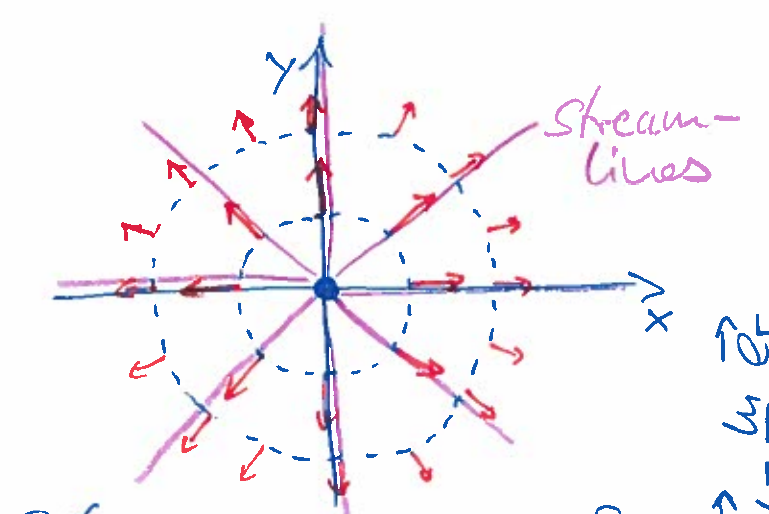
\includegraphics[width=.5\textwidth]{week3/radial-streamlines}\\
    \caption{}
    \label{fig:radial-streamlines}
\end{figure}

\textbf{Play 2:} method of images. Source flow in front of a wall. See \fref{fig:mirror-source}.

Boundary condition: no flow through the wall; only tangential component.
\begin{equation}
\phi(x,y) = \frac{m}{2\pi}\ln\sqrt{(x+a)^2+y^2} + \frac{m}{2\pi}\ln\sqrt{(x-a)^2+y^2}
\end{equation}
\begin{figure}[!h]
    \centering
    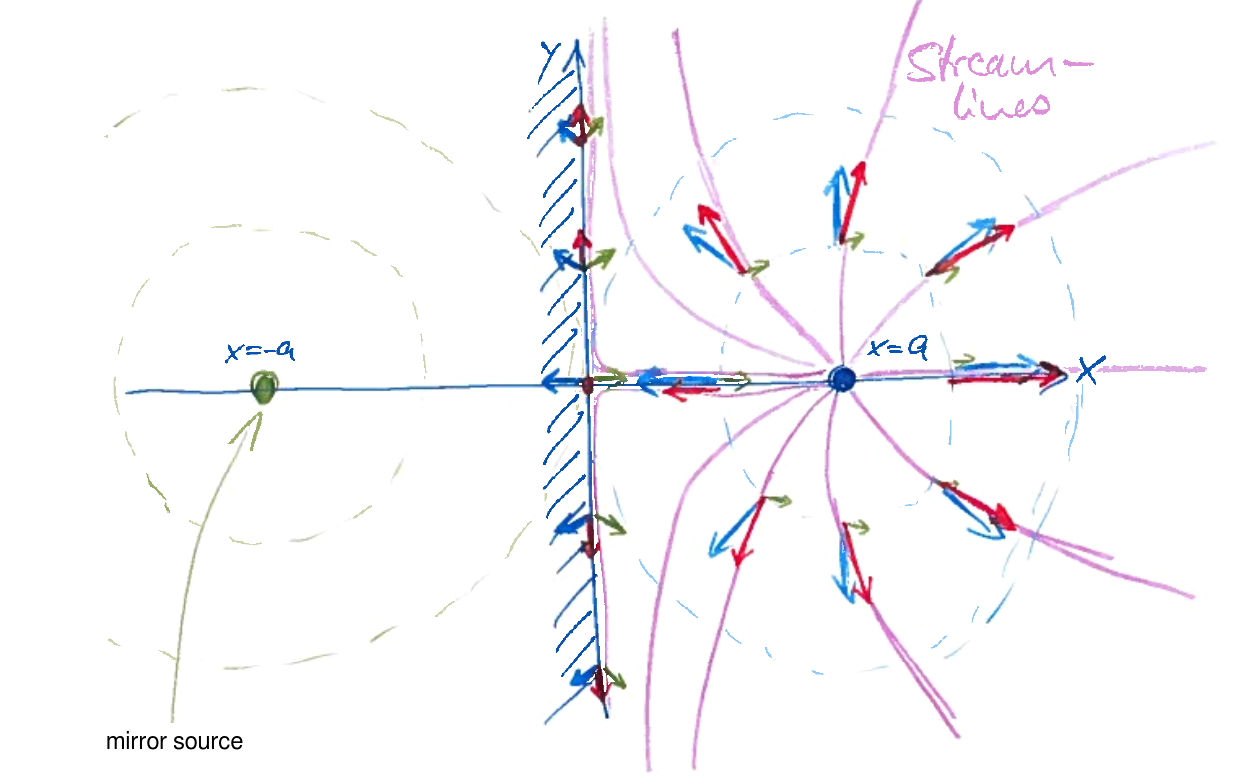
\includegraphics[width=.6\textwidth]{week3/mirror-source}\\
    \caption{}
    \label{fig:mirror-source}
\end{figure}

\textbf{Play 3:} flow past a 2-dimensional half-body. See \fref{fig:half-body}.
\begin{align}
\Phi &= u_\infty x + \frac{m}{2\pi}\ln\sqrt{x^2+y^2}\\
\leadsto
\ppdiff{\Phi}{x}+\ppdiff{\Phi}{y} &= 0
\end{align}
\begin{align}
u_x(x,y) &= u_\infty + \frac{m}{2\pi}\frac{x}{x^2+y^2}\\
u_y(x,y) &= u_\infty + \frac{m}{2\pi}\frac{y}{x^2+y^2}
\end{align}

Engineering flow interpretations:
\begin{enumerate}
\item An example of the beginning of the half-body is the leading edge of an airfoil
\item pedestrian on a bridge looking down: front part of a bridge pier
\item flow over a cliff
\end{enumerate}

\begin{figure}[!h]
    \centering
    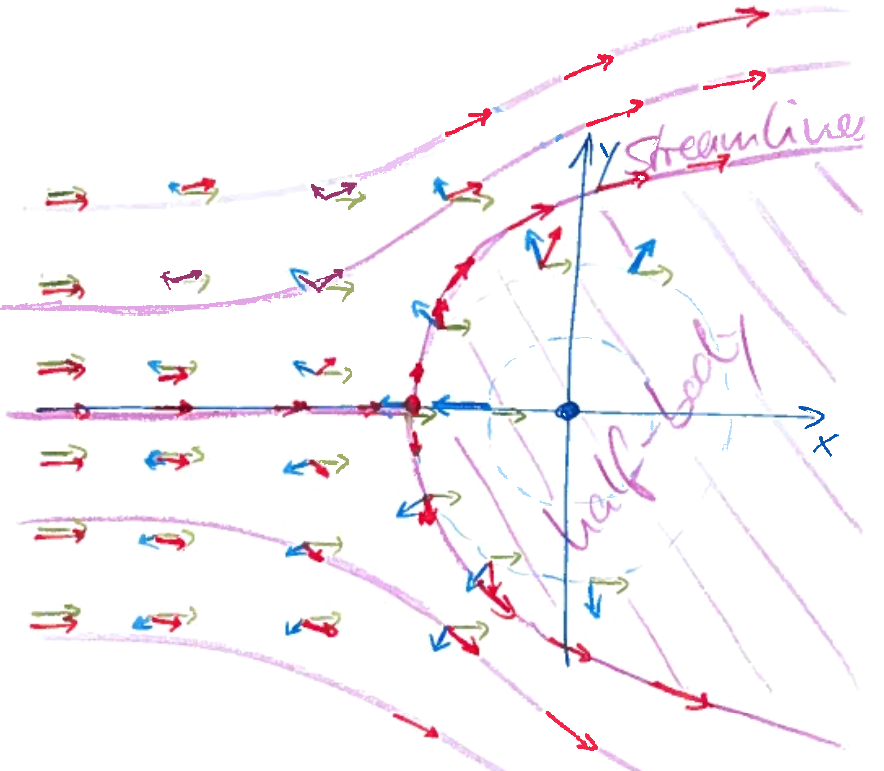
\includegraphics[width=.6\textwidth]{week3/half-body}\\
    \caption{}
    \label{fig:half-body}
\end{figure}

\textbf{Play 4:} numerial solutions (KCD section 6: Computational Fluid Dynamics)

\textbf{Play 5:} "beauty of mathematics". Conformal mappings.
Complex potential
\begin{equation}
w(z) = \phi(x,y)+i\psi(x,y)
\end{equation}
where $z=x+iy$.

Velocity:
\begin{align}
\diff{w(z)}{z} &= \diff{w(z)}{z}\biggm\vert_{dz=dx} = \pdiff{\phi}{x}+i\pdiff{\psi}{x} = u_x-iu_y \\
&= \diff{w(z)}{z}\biggm\vert_{dz=idy} = \pdiff{\phi}{y}+i\pdiff{\psi}{y} = \pdiff{\psi}{y}-i\pdiff{\phi}{y} = u_x-iu_y
\end{align}

Differentiable example 1:
\begin{equation}
w(z)=u_\infty z = u_\infty(x+iy) = u_\infty x + iu_\infty y
\end{equation}
describes the constant flow $\vec{u}=u_\infty \vec{e}_x$.

Differentiable example 2:
\begin{align}
w(z) &= \frac{m}{2\pi}\ln z = \frac{m}{2\pi} \ln(x+iy)\\
&= \frac{m}{2\pi}\ln(re^{i\theta}\\
&= \frac{m}{2\pi}\ln r +\frac{m}{2\pi}\ln e^{i\theta}\\
&= \frac{m}{2\pi}\ln\sqrt{x^2+y^2} + i\frac{m}{2\pi}\theta
\end{align}
The two terms in the last line is the velocity field and stream function of a radial source flow (see "play 1").

Differentiable example 3:
\begin{align}
w(z) &= \frac{A}{2}z^2 = \frac{A}{2}(x+iy)^2\\
&= \frac{A}{2}(x^2-y^2)+iAxy
\end{align}

Differentiable example 4:
\begin{align}
w(z) &= \phi(x,y) +i\psi(x,y) = u_\infty x\left(1+\frac{R^2}{x^2+y^2}\right) + iu_\infty y \left(1-\frac{R^2}{x^2+y^2}\right) \\
& =u_\infty(x+iy) + u_\infty R^2\frac{x-iy}{x^2+y^2} \\
&= u_\infty(x+iy)+\frac{u_\infty R^2}{x+iy}\\
&= u_\infty\left(z+\frac{R^2}{z}\right)
\end{align}

flow around cylinder with radius $R$:
\begin{equation}
w(z)=u_\infty\left(z+\frac{R^2}{z}\right)
\end{equation}
change of variable:
\begin{equation}
z)z(\tilde{z})
\end{equation}
Example:
\begin{align}
\tilde{z} &= (z+z_0)+\frac{1}{z+z_0}\\
\leadsto
w_\mathrm{new\ obstacle}(\tilde{z}) &= w_\mathrm{cylinder}(z(\tilde{z}))
\end{align}

\begin{shaded}
Should we include the figure on the left half of page 43 here?
\end{shaded}


\begin{framed}
\textbf{Remark:} other applications of conformal mappings

\textbf{Electrostatics}
\begin{equation}
\Delta\phi = \vec{\nabla}\cdot\vec{\nabla\phi=0}
\end{equation}

\textbf{Heat flux}
\begin{equation}
\pdiff{T(x,y)}{t}=\kappa\vec{\nabla}\cdot\vec{\nabla}T(x,y) \Rightarrow \Delta T(x,y) = 0
\end{equation}
\end{framed}

\section{Forces on a 2-dimensional body (45-63)}

\begin{framed}
Ideal potential flows:
\begin{equation}
\vec{\nabla}\cdot\vec{v}=0=\vec{\nabla}\times\vec{v}\Rightarrow\vec{\nabla}\cdot\vec{\nabla}\phi = \left(\ppdiff{}{x}+\ppdiff{}{y}\right)\phi=0
\end{equation}
Where is the Euler equation? Do we need it?
\end{framed}

Euler equation:
\begin{equation}
\rho \left(\pdiff{\vec{v}}{t}+\left(\vec{v}\cdot\vec{\nabla}\right)\vec{v}\right) = \rho \vec{f} - \vec{\nabla}p + \mu\left(\vec{\nabla}\cdot\vec{\nabla}\right)\vec{v}
\end{equation}

Reduce to Bernoulli equation:
\begin{equation}
\vec{\nabla}\left(\frac{\rho}{2}\vec{v}^2+p\right)=0
\end{equation}

With the Bernoulli equation (leftover from the Euler equation) we can calculate the force on the "obstacle" (\fref{fig:2dim-body}) from the surrounding flow:

\begin{align}
\vec{F} &= \int_{S(v)}(-p(\vec{r}))d\vec{A} = -\int_{S(v)}\left(p_0-\frac{\rho}{2}\vec{v}^2(\vec{r})\right)d\vec{A} \\
&= \frac{\rho}{2}\int_{S(v)}\vec{v}^2(\vec{r})d\vec{A}\\
&= L\vec{e}_y +\underbrace{D\vec{e}_x}_{=0}
\end{align}
where $\vec{L}$ is the lift force and $\vec{D}$ is the drag force. The last term equals zero because there is no friction.

\begin{figure}[!h]
    \centering
    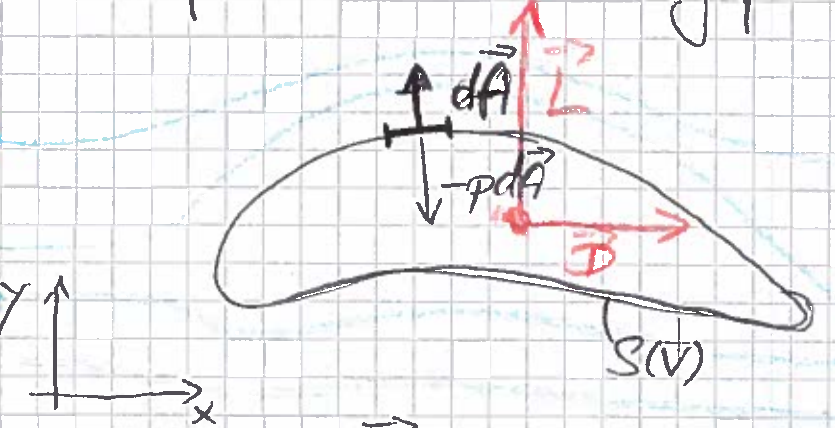
\includegraphics[width=.5\textwidth]{week4/2dim-body}\\
    \caption{}
    \label{fig:2dim-body}
\end{figure}

\begin{shaded}
I skipped page 45a and the solution of an old exam problem: pages 46, 46a-46d.
\end{shaded}

\begin{figure}[!h]
    \centering
    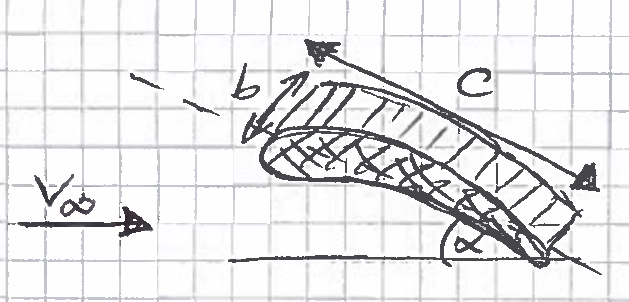
\includegraphics[width=.4\textwidth]{week4/generic-lift2}\\
    \caption{}
    \label{fig:generic-lift2}
\end{figure}

Lift coefficient
\begin{equation}
C_L = \frac{L}{\frac{\rho}{2}v_\infty^2 b c}
\end{equation}
Drag coefficient:
\begin{equation}
C_D = \frac{D}{\frac{\rho}{2}v_\infty^2 b c}
\end{equation}

\begin{figure}[!h]
    \centering
    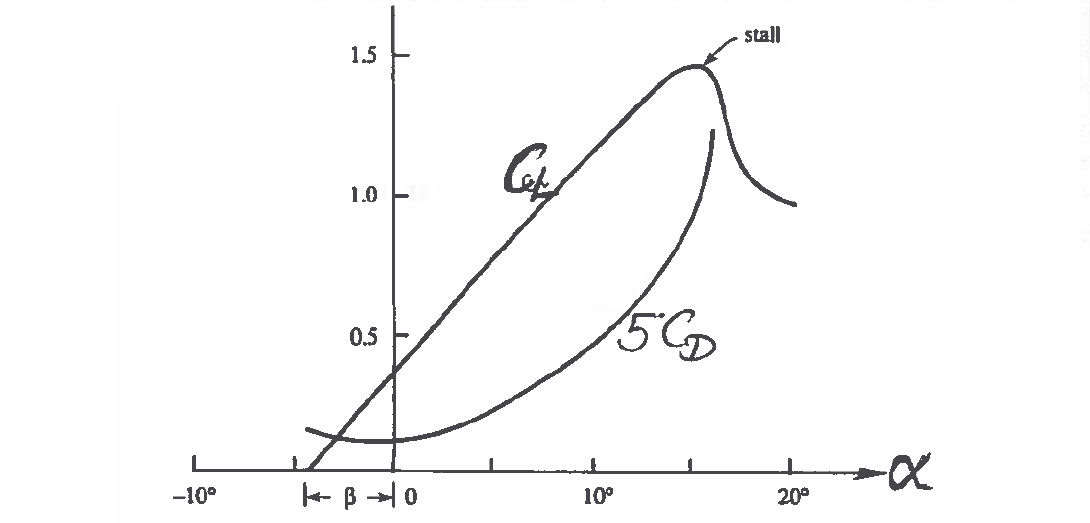
\includegraphics[width=.5\textwidth]{week4/generic-lift}\\
    \caption{}
    \label{fig:generic-lift}
\end{figure}


\subsection{Turbine blade}
Explain how the lift force pulls the rotor blade of a wind turbine forward. See \fref{fig:turbine-blade}.
\begin{figure}[!h]
    \centering
    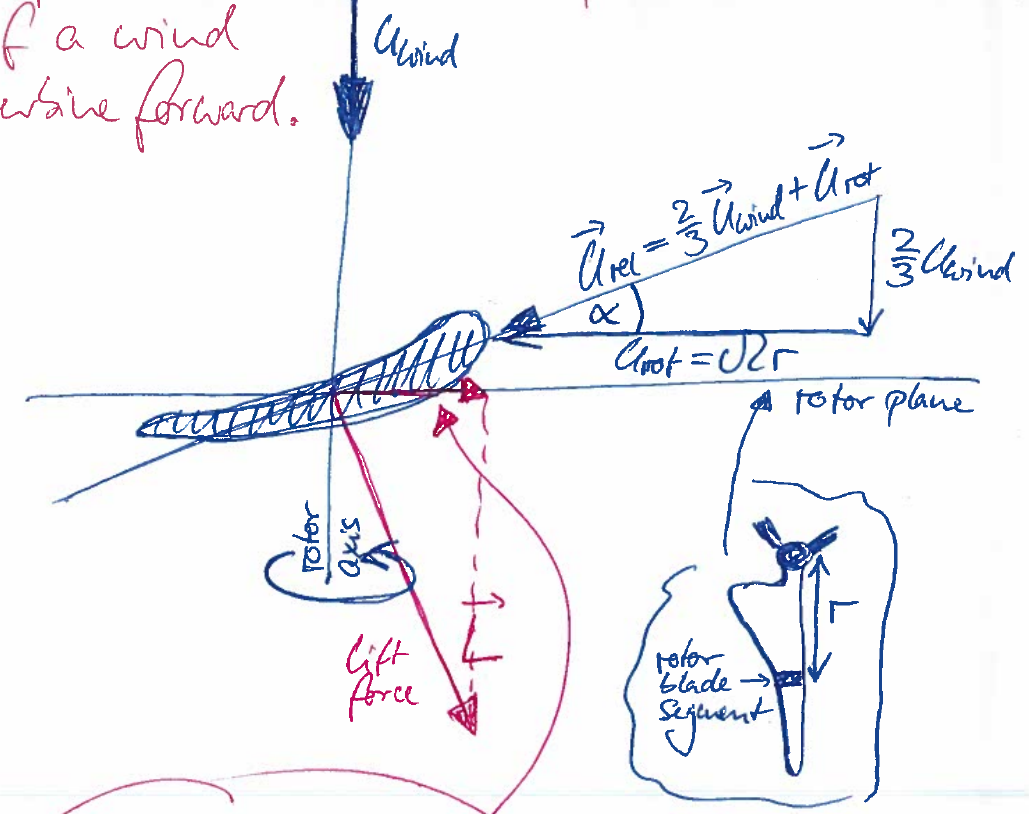
\includegraphics[width=.6\textwidth]{week4/turbine-blade}\\
    \caption{}
    \label{fig:turbine-blade}
\end{figure}


\subsection[Sailing against the wind]{Sailing against the wind (KCD 14.9)}
People have sailed without the aid of an engine for thousands of years and have known
how to reach an upwind destination. Actually, it is not possible to sail exactly against the
wind, but it is possible to sail at z 40e45$^\circ$ to the wind. Figure 14.29 shows how this is
made possible by the aerodynamic lift on the sail, which is a piece of stretched and stiffened
cloth. The wind speed is U, and the sailing speed is V, so that the apparent wind speed rela-
tive to the boat is Ur. If the sail is properly oriented, this gives rise to a lift force perpendicular
to Ur and a drag force parallel to Ur. The resultant force F can be resolved into a driving
component (thrust) along the motion of the boat and a lateral component. The driving
component performs work in moving the boat; most of this work goes into overcoming
the frictional drag and in generating the gravity waves that radiate outward from the hull.
The lateral component does not cause much sideways drift because of the shape of the
hull. It is clear that the thrust decreases as the angle q decreases and normally vanishes
when $\theta$ is $\approx$ 40e45$^\circ$ . The energy for sailing comes from the wind field, which loses kinetic
energy after passing the sail.

\begin{figure}[!h]
    \centering
    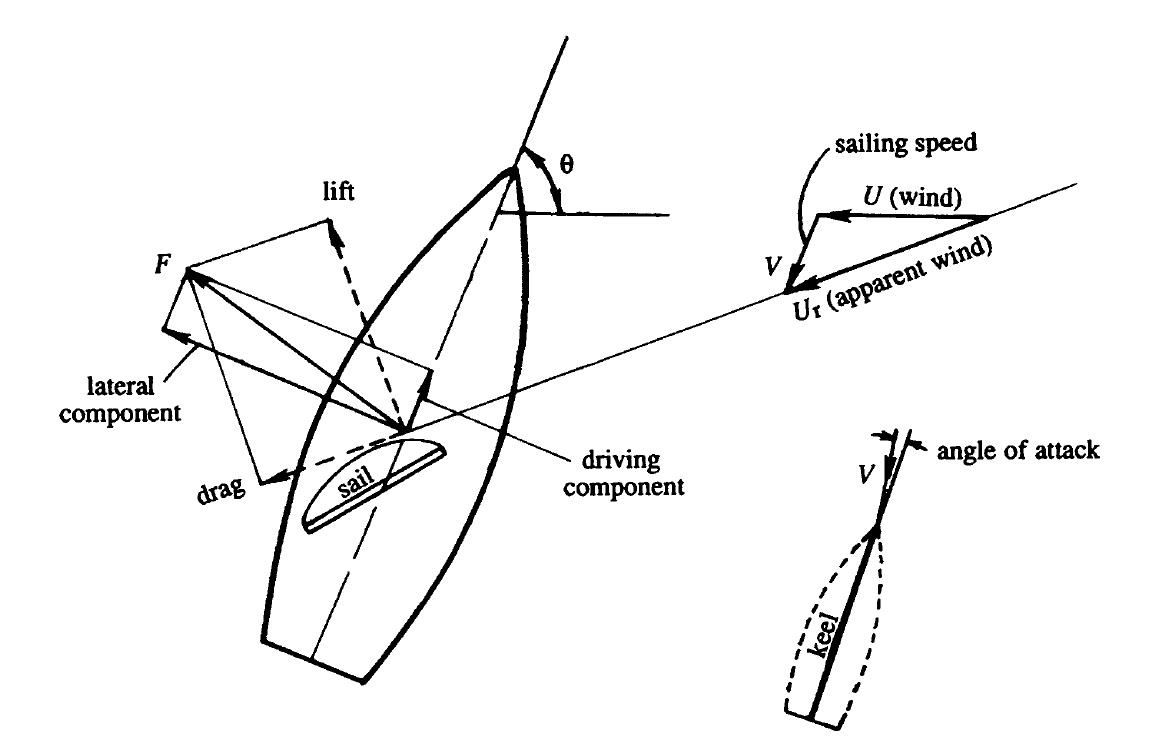
\includegraphics[width=.6\textwidth]{week4/sailing-wind}\\
    \caption{Principle of sailing against the wind. A small component of the sail’s lift pushes the boat forward at an angle q < 90$^\circ$ to the wind. Thus by traversing a zig-zag course at angles $\pm\theta$, a sailboat can reach an upwind destination. A sailboat’s keel may make a contribution to its upwind progress too.}
    \label{fig:sailing-wind}
\end{figure}

\newpage
\subsection{Reynolds number}
Fluid around a cylinder can create several real flow patterns. See \fref{fig:reynolds-cylinder}.

\begin{figure}[p]
    \centering
    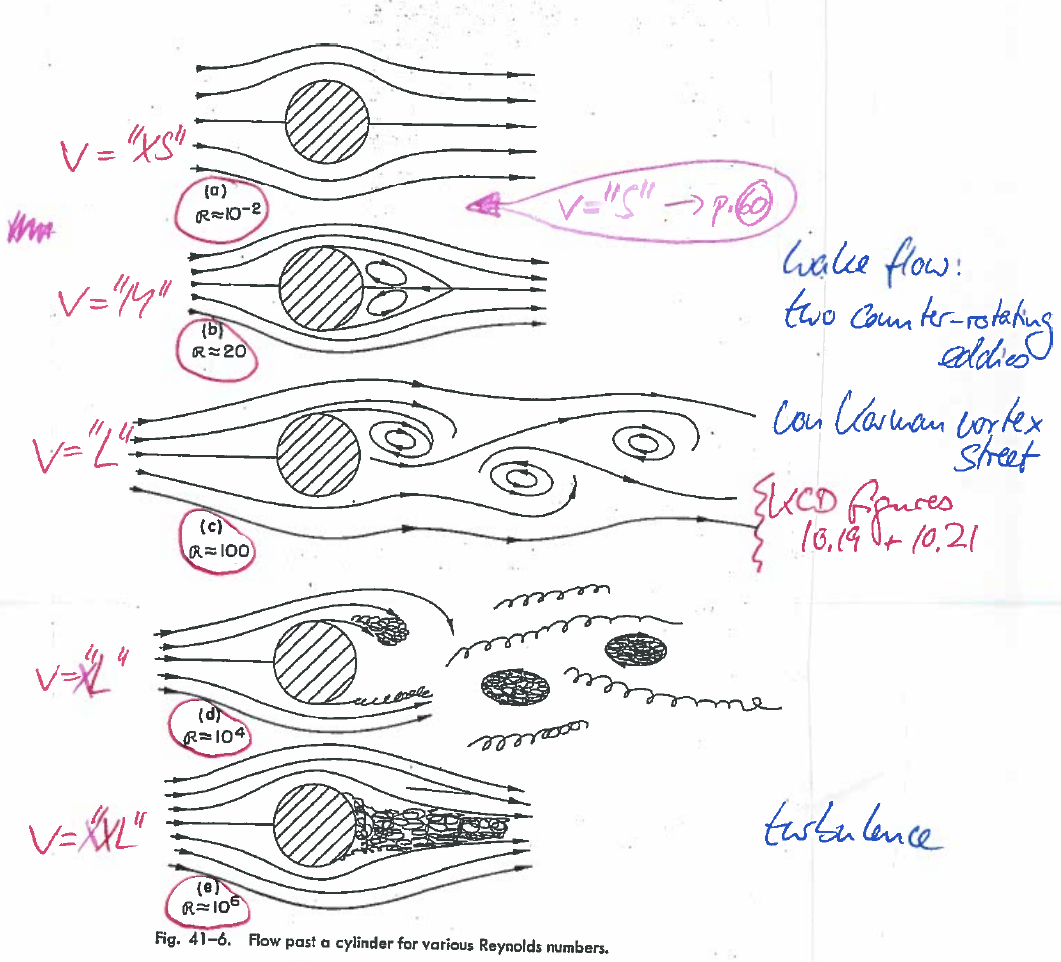
\includegraphics[width=\textwidth]{week4/reynolds-cylinder}\\
    \caption{}
    \label{fig:reynolds-cylinder}
\end{figure}

\textbf{Questions:}
\begin{enumerate}
\item why so many different flows?
\item what causes and characterizes them?
\end{enumerate}
Certainly friction, i.e. viscosity, will have something to do with it.

\begin{align}
0 &= \rho_0 \left[\pdiff{\vec{v}}{t}+\left(\vec{v}\cdot\vec{\nabla}\right)\vec{v}\right] + \vec{\nabla}p - \mu\Delta \vec{v} \\
&= \rho_0\left[\frac{V}{T}\pdiff{\vec{v}'}{t'}+\frac{V^2}{L}\left(\vec{v}'\cdot\vec{\nabla}'\right)\vec{v}'\right] + \frac{\rho_0 V^2}{L}\vec{\nabla}'p'-\mu\frac{V}{L^2}\Delta'\vec{v}' \\
&= \rho_0\frac{V^2}{L} \left\lbrace \pdiff{\vec{v}'}{t'}+\left(\vec{v}'\cdot\vec{\nabla}'\right)\vec{v}'+\vec{\nabla}'p'-\frac{\mu}{\rho_0 LV} \Delta'\vec{v}' \right\rbrace
\end{align}
where $L$ is the characteristic length, $V$ is the characteristic velocity, $T=L/V$ is the characteristic time, and $P=\rho_0V^2$ the characteristic pressure.

Reynolds number:
\begin{equation}
Re = \frac{\rho_0 L V}{\mu}
\end{equation}

\begin{framed}
\textbf{Remark:} law of similarity

If two flows have the same geometry (object) and the same Reynolds number, but a different absolute scale it means that the two flows are similar (identical, except for a scale transformation). Applications of this is wind tunnel experiments of air wings, wind turbine blades, cars, etc.
\end{framed}

The Reynolds number
\begin{equation}
Re = \frac{\rho_0 L V}{\mu} = \frac{\rho_0 V^2/L}{\mu V/L},
\end{equation}
is the inertia force density divided by the friction force density.

\begin{figure}[p]
    \centering
    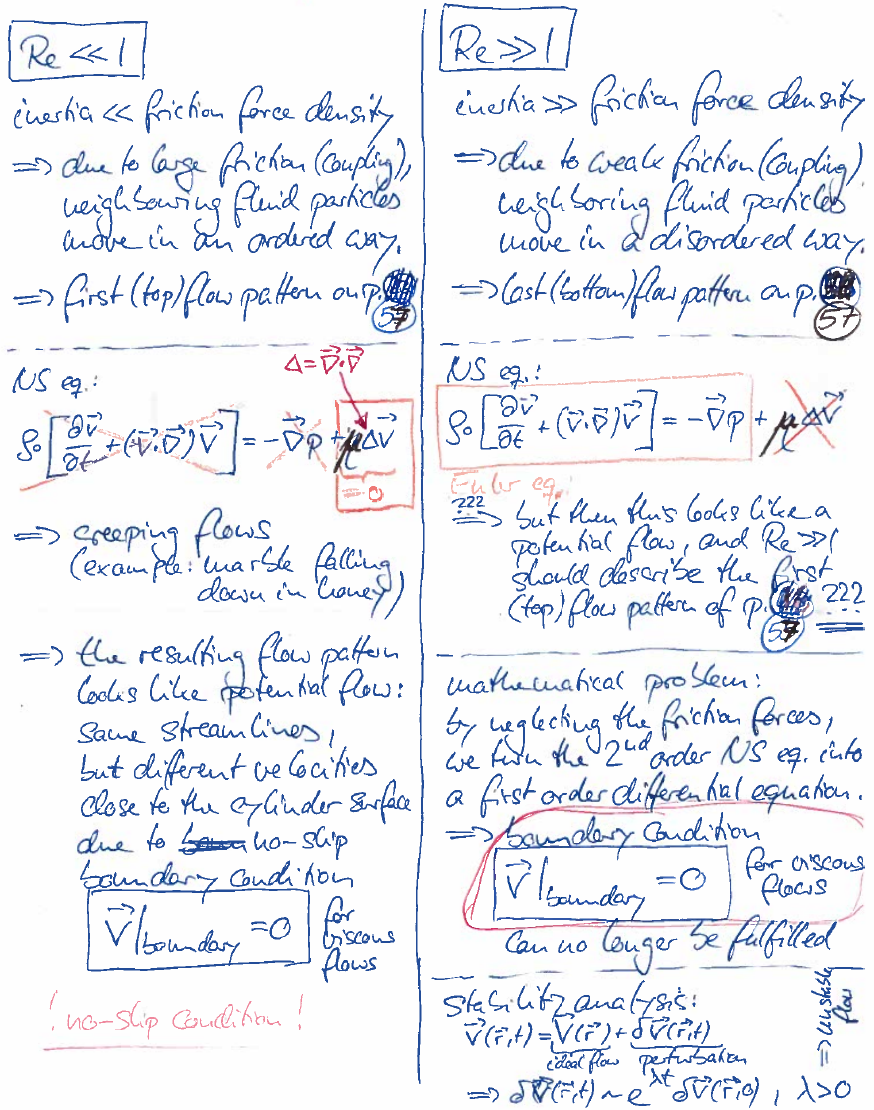
\includegraphics[width=\textwidth]{week4/reynolds-numbers}\\
    \caption{This should be presented in text in a better way.}
    \label{fig:reynolds-numbers}
\end{figure}

\begin{figure}[p]
    \centering
    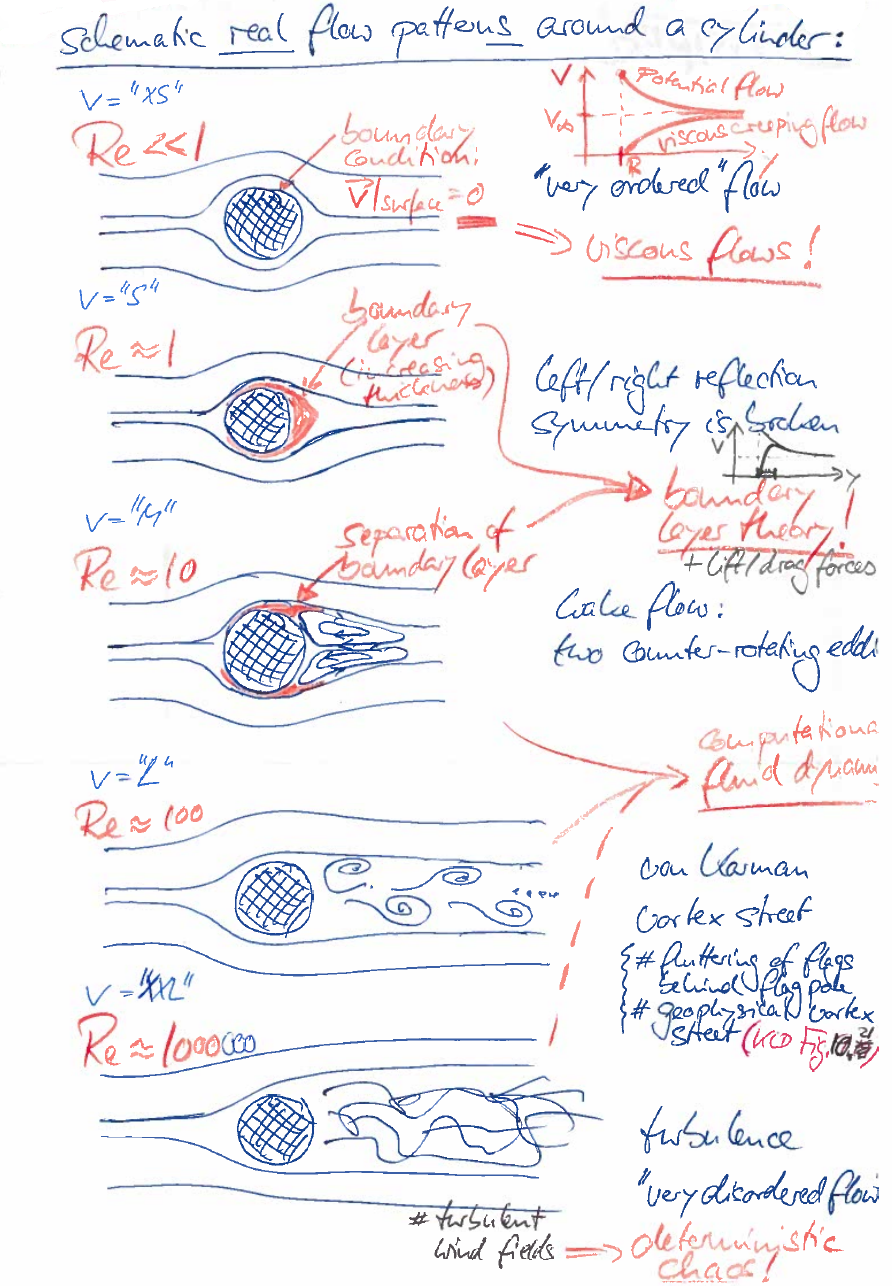
\includegraphics[width=\textwidth]{week4/schematic-flows}\\
    \caption{}
    \label{fig:schematic-flows}
\end{figure}


\newpage
\subsection{Viscous pipe flow}

\begin{figure}[ht]
    \centering
    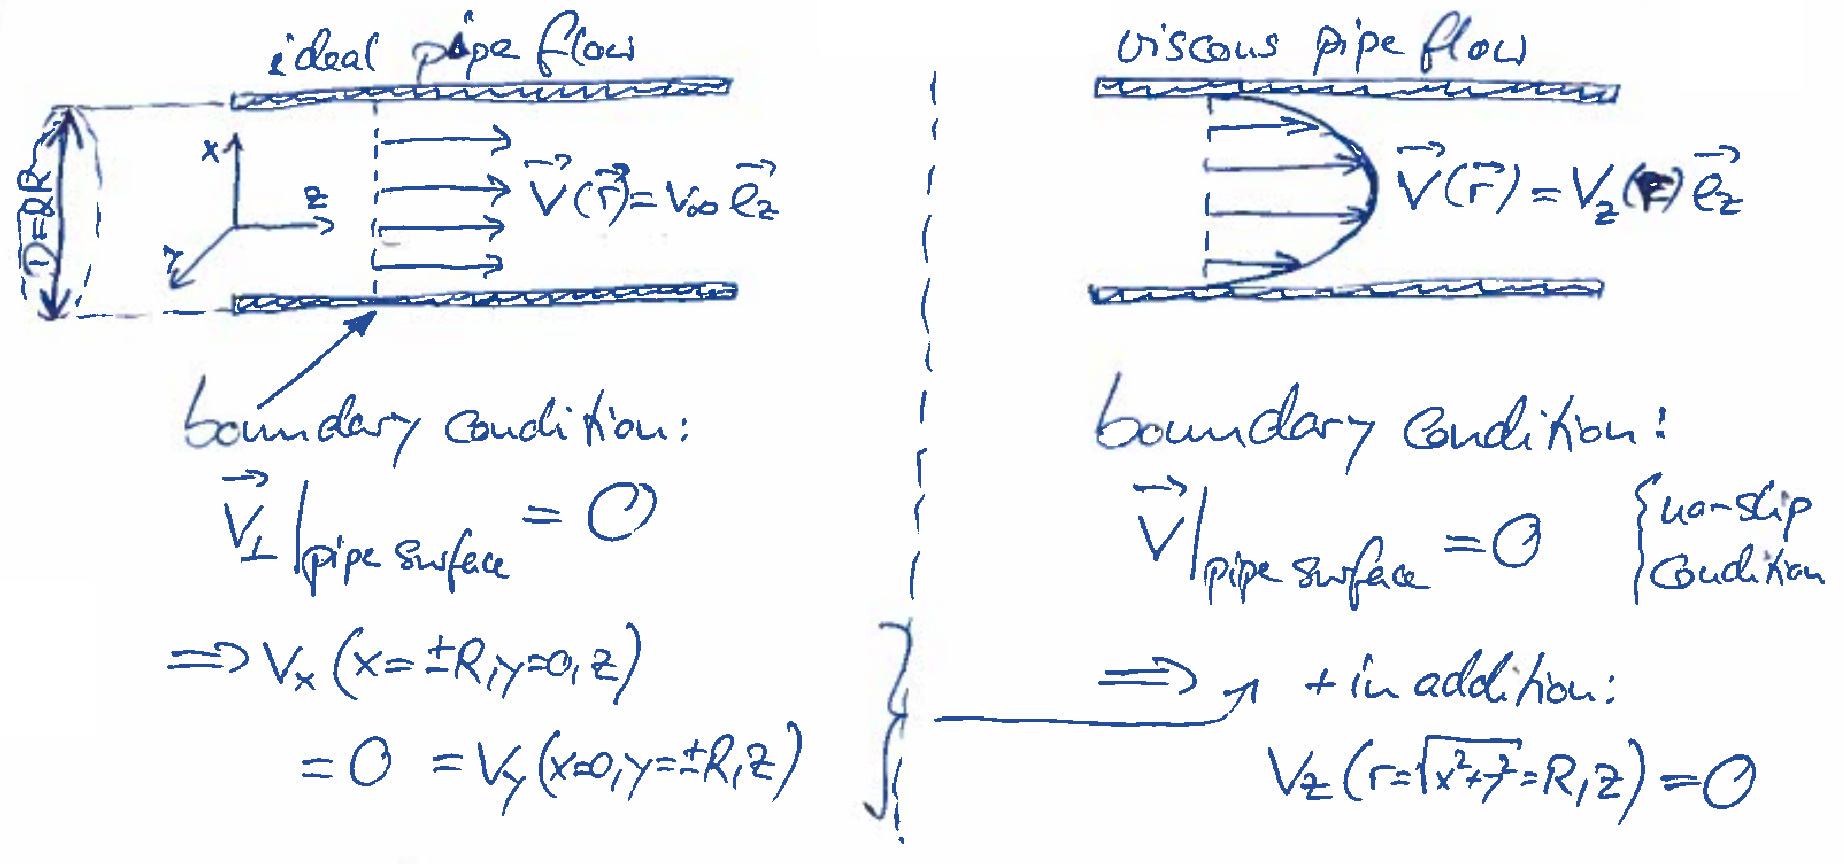
\includegraphics[width=\textwidth]{week4/viscous-pipe-flow}\\
    \caption{}
    \label{fig:viscous-pipe-flow}
\end{figure}

Task: calculate velocity profile $v_z=v_z(r)$ for the viscous pipe flow.

Navier-Stokes equation
\begin{equation}
\rho_0\underbrace{\pdiff{\vec{v}}{t}}_{=0}+\rho_0\underbrace{\left(\vec{v}\cdot\vec{\nabla}\right)}_{=0}\vec{v} = \underbrace{f_\mathrm{ext}}_{=0}-\vec{\nabla}p+\mu\left(\vec{\nabla}\cdot\vec{\nabla}\right)\vec{v}
\end{equation}

\begin{align}
0 &= -\vec{\nabla}p + \mu\left(\ppdiff{}{x}+\ppdiff{}{y}\right)v_z\vec{e}_z\\
\leadsto
\left(\vec{\nabla}p\right)_x &= \left(\vec{\nabla}p\right)_y = 0 \\
\leadsto
p &= p(z)
\end{align}

\begin{align}
\mu\Delta v_z(r) &= \frac{\mu}{r}\pdiff{}{r}\left(r\pdiff{v_z(r)}{r}\right) \\
&= \pdiff{p(z)}{z} \require \mathrm{constant}
\end{align}

\begin{align}
\pdiff{p(z)}{t}&=c \\
\leadsto
p(z) &= cz+d \\
&= \frac{p(z=L)-p(z=0)}{L}z+p(z=0)\\
&= -\frac{\Delta p}{L}z + p(z=0)
\end{align}

\begin{align}
\frac{\mu}{r}\pdiff{}{r}\left(r\pdiff{v_z(r)}{r}\right) &= c = -\frac{\Delta p}{L} \\
\leadsto
r\pdiff{v_z(r)}{r} &= -\frac{\Delta p}{\mu L}\frac{r^2}{2} + D_1 \\
\leadsto
v_z(r) &= -\frac{\Delta p}{4\mu L}r^2 + D_1 \ln r + D_ 2 \\
\leadsto
v_z(r) &= \frac{\Delta p}{4\mu L}\left( R^2 - r^2\right)
\end{align}

Fluid mass per time passing through pipe cross-section:
\begin{equation}
\diff{M}{t} = \int_0^R\rho_0 v_z(r)2\pi r dr = \frac{\pi\rho_0 R^4\Delta p}{8\mu L}
\end{equation}
This is the Hagen-Poiseuille law.
\begin{framed}
\textbf{Remark:} this law allows to determine the viscosity:
\begin{equation}
\left\lbrace \underbrace{\rho_0,R,L}_\mathrm{known} \quad,\quad \underbrace{\Delta p,\diff{M}{t}}_\mathrm{measured} \right\rbrace \Rightarrow \mu
\end{equation}
\end{framed}

\begin{framed}
\textbf{Remark:} "Ohm's Law"

\begin{align}
\Delta p = \Delta u \ &,\quad \diff{M}{t} = I\\
\leadsto
I &= \frac{\pi\rho_0 R^4}{8L\mu}
\end{align}

{\center
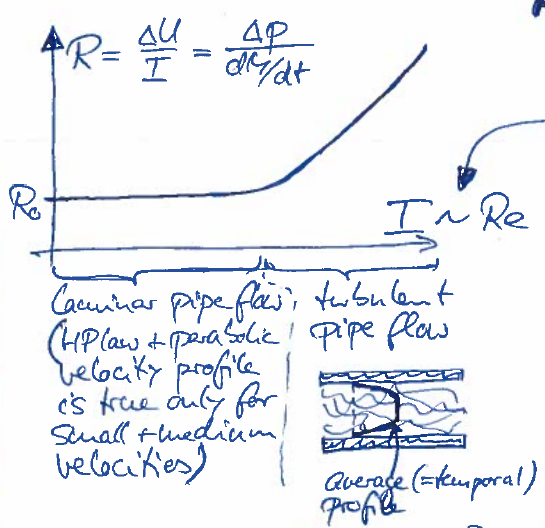
\includegraphics[width=.4\textwidth]{week4/ohms-law}\\
}

\begin{equation}
R = R_0\cdot f(Re)
\end{equation}
with
\begin{equation}
f(Re\rightarrow0)=1
\end{equation}
we conclude that turbulence increases pipe resistance. This is important for the operation of oil and gas pipelines.
\end{framed}




\newpage
\subsection{Boundary layers}

\begin{figure}[ht]
    \centering
    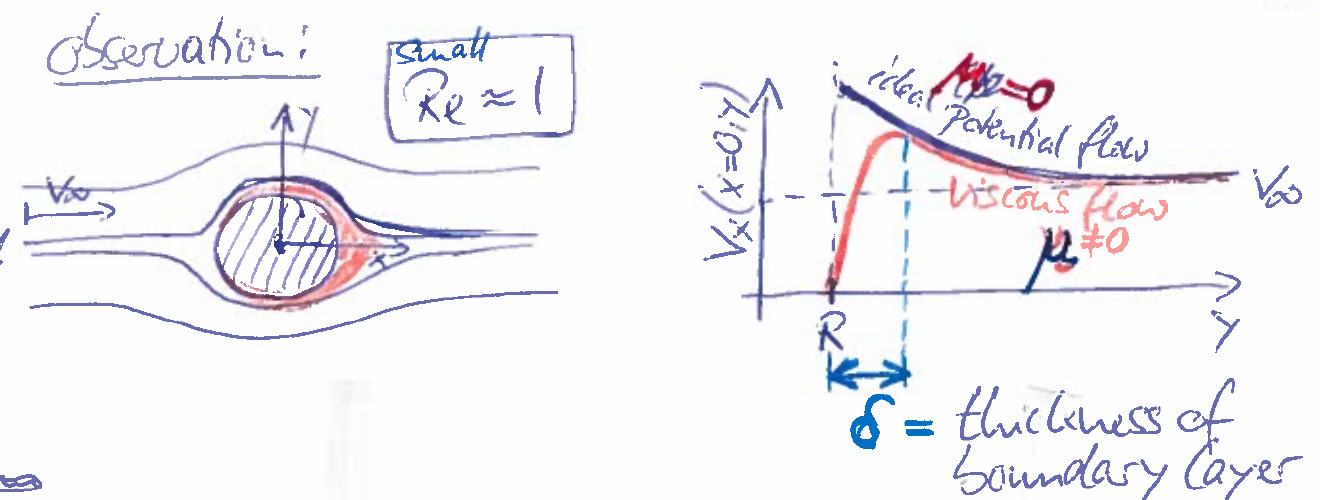
\includegraphics[width=\textwidth]{week4/boundary-layers}\\
    \caption{}
    \label{fig:boundary-layers}
\end{figure}

Idea of boundary layer theory:
\begin{enumerate}
\item within the boundary layer the velocity increases from zero to the ideal flow velocity
\item inside the boundary layer we use the Navier-Stokes equation (with friction)
\item outside the boundary layer we use the Euler equation without friction i.e. ideal potential flow
\item at the boundary surface we match the inside solution with the outside solution
\end{enumerate}

Derivation of the (laminar) boundary layer equations. Approximation to the Navier-Stokes equation inside the boundary layer. See \fref{fig:laminar-boundary}.

\begin{figure}[ht]
    \centering
    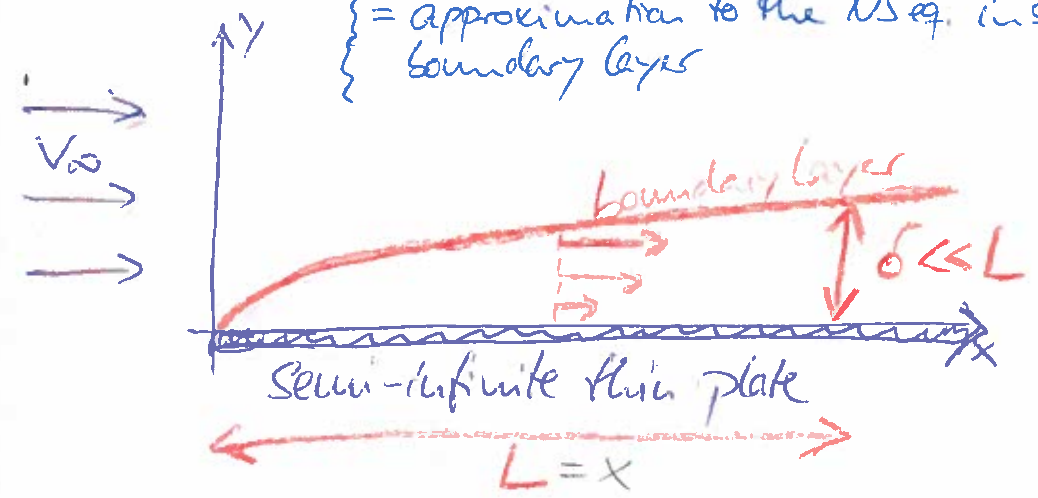
\includegraphics[width=.7\textwidth]{week4/laminar-boundary}\\
    \caption{}
    \label{fig:laminar-boundary}
\end{figure}

In the following we determine $\delta = \delta(x)$ (\fref{fig:laminar-boundary}) without solving the Navier-Stokes equation.

Incompressible flow:
\begin{align}
\vec{\nabla}\cdot\vec{v} &= \pdiff{v_x}{x} + \pdiff{v_y}{y} = 0 \\
&= \mathcal{O} \left(\frac{v_\infty}{L}\right) + \mathcal{O} \left(\frac{v_y}{\delta}\right) \\
\leadsto
\mathcal{O}(v_y) &= \delta\frac{v_\infty}{L} = \frac{\delta}{L}v_\infty
\end{align}

Navier-Stokes equation (x-component):
\begin{equation}
v_x\pdiff{v_x}{x} + v_y\pdiff{v_x}{y} = -\frac{1}{\rho_0}\pdiff{p}{x} + \frac{\mu}{\rho_0}\ppdiff{v_x}{x} + \frac{\mu}{\rho_0}\ppdiff{v_x}{y}
\end{equation}
\begin{equation}
\mathcal{O} \left(\frac{v_\infty^2}{L}\right) \require \mathcal{O} \left(\frac{\mu}{\rho_0}\frac{v_\infty}{\delta^2}\right)
\end{equation}

\begin{equation}
\left(\frac{\delta}{L}\right)^2 \sim \frac{\mu}{\rho_0 L v_\infty} = \frac{1}{Re}
\end{equation}
The larger the Reynolds number, the thinner the boundary layer. This holds for $Re \leq \SI{1e5}{}-\SI{1e6}{}$, above that the boundary layer becomes turbulent, and is no longer laminar. 

\begin{equation}
\delta(x) \sim \sqrt{\frac{\mu x}{\rho_0 v_\infty}}
\end{equation}


Navier-Stokes equation (y-component):
\begin{equation}
v_x\pdiff{v_y}{x} + v_y\pdiff{v_y}{y} = -\frac{1}{\rho_0}\pdiff{p}{y} + \frac{\mu}{\rho_0}\ppdiff{v_y}{x} + \frac{\mu}{\rho_0}\ppdiff{v_y}{y}
\end{equation}

\begin{equation}
\pdiff{p}{y} = 0 \Rightarrow p = p(x)
\end{equation}


\textbf{Prandtl equations:} laminar boundary layer equations
\begin{align}
v_x\pdiff{v_x}{x}+v_y\pdiff{v_x}{y} &= -\frac{1}{\rho_0}\pdiff{p(x)}{x}+\frac{\mu}{\rho_0}\ppdiff{v_x}{y} \\
\pdiff{v_x}{x}+\pdiff{v_y}{y}&=0
\end{align}

\textbf{Example:} Solution of Prandtl equations for laminar boundary flow around semi-infinite plate

\begin{equation}
p=p(x) \Rightarrow p(x)|_\mathrm{inside} = p(x)|_\mathrm{outside}
\end{equation}

Outside boundary layer:
\begin{align}
v_x|_\mathrm{outside} &= v_x = v_\infty = \mathrm{constant} \\
v_y|_\mathrm{outside} &= 0
\end{align}

Bernoulli equation:
\begin{align}
p(x) + \frac{\rho_0}{2}v_x^2 &= \mathrm{constant}\\
\leadsto
p(x) &= \mathrm{constant} \\
\leadsto
\pdiff{p(x)}{x} &= 0
\end{align}

Similarity ansatz:
\begin{equation}
v_x(x,y) = v_\infty g\left(\frac{y}{\delta(x)}\right)
\end{equation}
Except for a rescaling with $\delta(x)$ the velocity $v_x(x,y)$ looks like the same for all $x$.
\begin{figure}[ht]
    \centering
    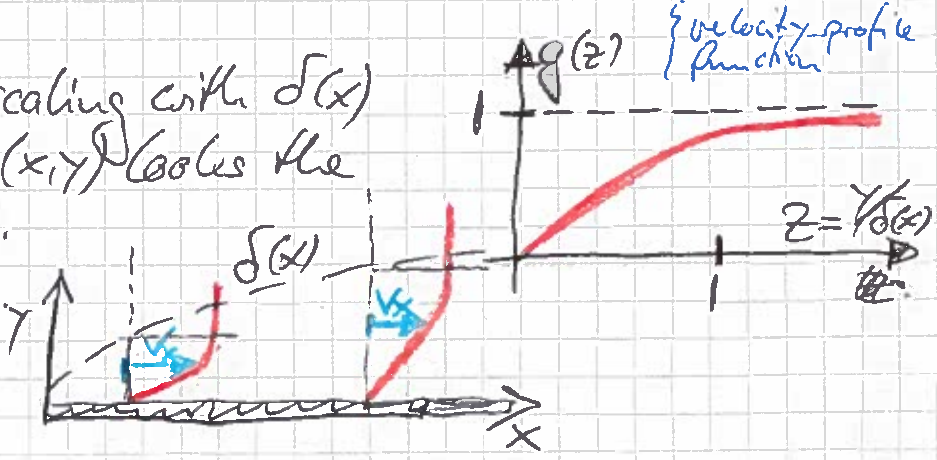
\includegraphics[width=.7\textwidth]{week4/boundary-ansatz}\\
    \caption{}
    \label{fig:boundary-ansatz}
\end{figure}


\noindent\makebox[\linewidth]{\rule{\textwidth}{0.5pt}}

\textbf{Question:} does the similarity ansatz work?

\begin{align}
\pdiff{v_x}{x}+\pdiff{v_y}{y} &= 0 \\
\leadsto
v_x = \pdiff{\psi}{y} \ &, \quad v_y = -\pdiff{\psi}{x}
\end{align}

\begin{equation}
\psi(x,y) = v_\infty\delta(x)f\left(\frac{y}{\delta(x)}\right)
\end{equation}

\begin{align}
v_x=\pdiff{\psi}{y} &= v_\infty\delta(x)\diff{f(z}{z}\diff{z}{y} \\
&= v_\infty \delta(x) \diff{f(z)}{z}\frac{1}{\delta(x)}\\
&= v_\infty \diff{f(z)}{z} \\
&\require v_\infty g(z)
\end{align}

\begin{equation}
f' = \diff{f(z)}{z}g(z)
\end{equation}

\noindent\makebox[\linewidth]{\rule{\textwidth}{0.5pt}}

\begin{align}
v_y &= -\pdiff{\psi}{x} \\
&=  -v_\infty\diff{\delta(x)}{x}f(z) - v_\infty \delta(x)\diff{f(z)}{z}\diff{z}{x}\\
&= v_\infty \left[-f + \frac{y f'}{\delta}\right] \diff{\delta(x)}{x}
\end{align}

\begin{align}
\pdiff{v_x}{x} &= \left(v_\infty f''\right)\left(\frac{-y}{\delta^2}\right)\diff{\delta(x)}{x} = -\frac{v_\infty y f''}{\delta^2}\diff{\delta(x)}{x} \\
\pdiff{v_x}{y} &= (v_\infty f'') \frac{1}{\delta} = \frac{v_\infty f''}{\delta} \\
\pdiff{v_x}{y} &= \frac{v_\infty f''}{\delta^2}
\end{align}

\begin{align}
\begin{split}
v_x\pdiff{v_x}{x} + v_y\pdiff{v_x}{y} - \frac{\mu}{\rho_0}\ppdiff{v_x}{y} &=
-(v_\infty f') \left(\frac{v_\infty y f''}{\delta^2} \diff{\delta(x)}{x}\right) \\
&\hspace{5mm} + \left(v_\infty\left[-f\frac{yf'}{\delta}\right]\diff{\delta(x)}{x}\right) \left(\frac{v_\infty f''}{\delta}\right) \\
&\hspace{5mm} -\frac{\mu}{\rho_0} \left(\frac{v_\infty f''}{\delta^2}\right)
\end{split} \\
&= -\frac{v_\infty^2}{\delta}\diff{\delta}{x} ff'' - \frac{\mu}{\rho_0} \frac{v_\infty}{\delta^2}f'''\\
&= 0
\end{align}

\begin{equation}
\frac{\rho_0 v_\infty}{\mu} \delta(x) \diff{\delta(x)}{x} = -\frac{f'''(z)}{f(z)f''(z)} \require c_1^2
\end{equation}

\begin{equation}
\delta\diff{\delta}{x} = \frac{1}{2}\diff{\delta^2}{x} = c_1^2\frac{\mu}{\rho_0v_\infty}\\
\end{equation}

\begin{equation}
\delta^2 = 2c_1^2 \frac{\mu}{\rho_0v_\infty}x + c_2
\end{equation}
$c_2=0$ since $\delta(x=0)=0$.

\begin{equation}
\delta(x) = c_1\sqrt{\frac{2\mu}{\rho_0v_\infty}x}
\end{equation}

\begin{equation}
\delta(x)=\sqrt{\frac{\mu}{\rho_0v_\infty}x}
\end{equation}
$c_1=\frac{1}{\sqrt{2}}$. Freedom of choice because of arbitrary definition of $\delta$; for example, $v_x(y=\delta)=0.99v_\infty$ or $v_x(x=\delta)=0.95v_\infty$.

This is the same result as the order of magnitude calculation when we calculated the x-component of the Navier-stokes equation earlier in this section.

\begin{equation}
f'''(z) +\frac{1}{2} f(z)f''(z) = 0
\end{equation}

\begin{equation}
f(z)\ddiff{f(z)}{z}+2\dddiff{f(z)}{z}=0
\end{equation}
This is Blasius' equation. A special case of the more general Falker-Skan equation.




















\subsection{Separation of boundary layers (64-65)}

Boundary condition at the wall:
\begin{equation}
v_x(x,y=0) = v_y(x,y=0)=0
\end{equation}

Prandtl equation (with pressure)
\begin{equation}
v_x\pdiff{v_x}{x}+v_y\pdiff{v_x}{y} = -\frac{1}{\rho_0}\pdiff{p}{x}+\frac{\mu}{\rho_0}\ppdiff{v_x}{y}
\end{equation}
If we are very close to the wall, the two terms on the left side equal zero. We then have
\begin{equation}
\pdiff{p(x,y=0)}{x}=\mu\ppdiff{v_x(x,y=0)}{y}
\end{equation}

\begin{figure}[!h]
    \centering
    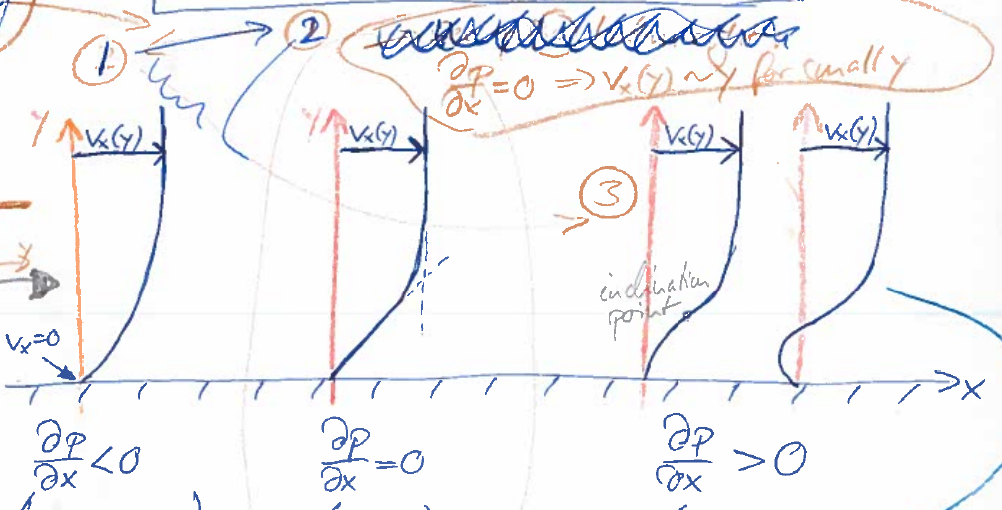
\includegraphics[width=.9\textwidth]{week5/wall-boundary}\\
    \caption{}
    \label{fig:wall-boundary}
\end{figure}

\begin{figure}[!h]
    \centering
    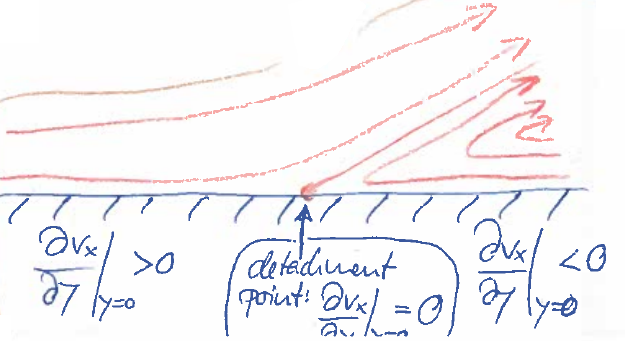
\includegraphics[width=.5\textwidth]{week5/detachment-point}\\
    \caption{}
    \label{fig:detachment-point}
\end{figure}

\newpage
\textbf{Example:} flow around cylinder

\begin{figure}[!h]
    \centering
    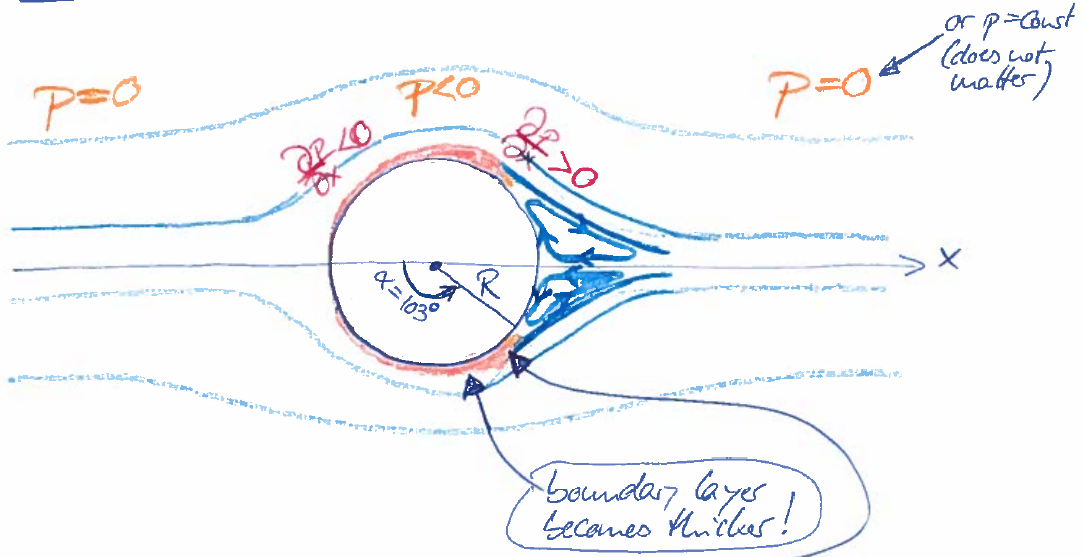
\includegraphics[width=.8\textwidth]{week5/cylinder-flow}\\
    \caption{}
    \label{fig:cylinder-flow}
\end{figure}

The detachment point is at the separation of the boundary layer. When $v\approx0$ there is no kinetic energy to run against the pressure gradient.

\begin{framed}
\textbf{Remark:} separation of boudnary layers is a big issue in mechanical engineering; for example: design of airfoils, wind-turbine blades etc.
{\center
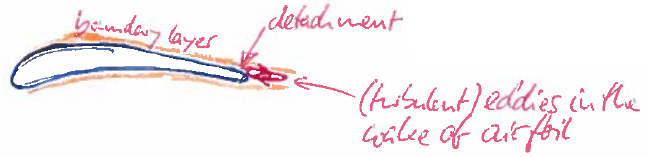
\includegraphics[width=.4\textwidth]{week5/detachment-eddies}\\
}
In case of separation the lift decreases, which can lead to airplane crash. It would also lead to a substantial rise in the overall drag (more friction). This would require more engine power and therefore more fuel for an airplane. For a wind turbine it would means less power generation.

Engineer's dream: construct airfoils without turbulent wake to mimic shark skin or fish scales.
\end{framed}

\subsection{Solution of Prandtl equations for free boundary layers (66-71)} 

\fref{fig:2d-laminar-jet} shows a 2-dimensional laminar jet flow generated from a flow through a long slit streaming into a resting fluid.

\begin{figure}[!h]
    \centering
    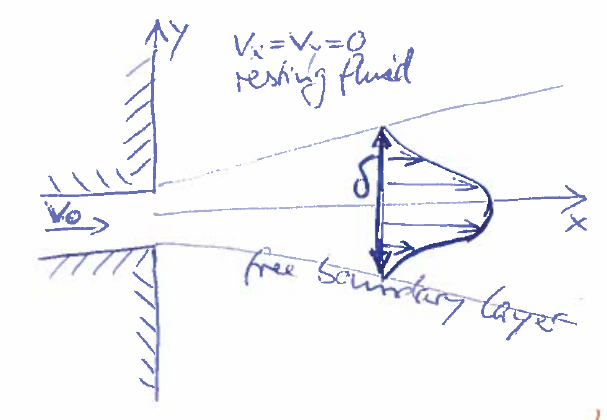
\includegraphics[width=.6\textwidth]{week5/2d-laminar-jet}\\
    \caption{}
    \label{fig:2d-laminar-jet}
\end{figure}

We use the Prandtl equations with the similarity ansatz:
\begin{equation}
v_x(x,y)=v_\mathrm{max}(x)g\left(\frac{y}{\delta(x)}\right)
\end{equation}

\begin{equation}
\pdiff{v_x}{x}+\pdiff{v_y}{y}=0 \Rightarrow v_x=\pdiff{\psi}{y},\quad v_y=-\pdiff{\psi}{x}
\end{equation}

\begin{equation}
\psi = v_\mathrm{max}(x)\delta(x)f\left(\frac{y}{\delta(x)}\right)
\end{equation}

\begin{equation}
\pdiff{\psi}{y}=v_\mathrm{max}\delta f'\frac{1}{\delta}=v_\mathrm{max}f'=v_\mathrm{max}g=v_x
\end{equation}

\begin{equation}
v_y=-\pdiff{\psi}{x}=-v'_\mathrm{max}\delta f-v_\mathrm{max}\delta'f-v_\mathrm{max}\delta f'\frac{(-y)\delta'}{\delta^2}
\end{equation}

\begin{align}
\partial_xv_x &= v'_\mathrm{max}f'+v_\mathrm{max}f''\frac{(-y)\delta'}{\delta^2} \\
\partial_yv_x &= v_\mathrm{max} f''\frac{1}{\delta}\\
\partial^2_xv_x &= \frac{v_\mathrm{max}}{\delta^2}f'''
\end{align}

\begin{align}
\begin{split}
v_x\partial_x v_x+v_y\partial_yv_x-\frac{\mu}{\rho_0}\partial^2_yv_x &= v_\mathrm{max}f'\left\lbrace v'_\mathrm{max}f' - v_\mathrm{max}\frac{y\delta'}{\delta^2}f''\right\rbrace \\
&\hspace{5mm}-\left\lbrace v'_\mathrm{max}\delta f + v_\mathrm{max}d'f-v_\mathrm{max}\frac{y\delta'}{\delta}f'\right\rbrace v_\mathrm{max}\frac{1}{\delta}f'' \\
&\hspace{5mm}-\frac{\mu}{\rho_0^2} \frac{v_\mathrm{max}}{\delta^2}f'''
\end{split}\\
\begin{split}
&= v_\mathrm{max}v'_\mathrm{max}f'^2-v_\mathrm{max}v'_\mathrm{max}ff''-v_\mathrm{max}^2\frac{\delta'}{\delta}ff'' \\
&\hspace{5mm}-\frac{\mu}{\rho_0}\frac{v_\mathrm{max}}{\delta^2}f'''\label{eq:free-boundary}
\end{split} \\
&\require0
\end{align}
All four terms in \eqref{eq:free-boundary} have the form $\alpha_i(x)\beta_i(x)$ for $(i=1,...,4)$. The sum of these four terms has to be zero. This means that $\alpha_1(x)\sim\alpha_2(x)\sim\alpha_3(x)\sim\alpha_4(x)$.

Ansatz:
\begin{align}
v_\mathrm{max}(x) &= c_1x^m\\
\delta(x) &= c_2 x^n
\end{align}

\begin{framed}
\textbf{Remark:} we expect $m<0$ (decreasing velocity with penetration depth) and $n>0$ (increasing thickness of jet with penetration depth).
\end{framed}

Sum of the 4 terms:
\begin{equation}
c_1^2mx^{2m-1}(f'^2-ff'')-c_1^2x^{2m}\frac{n}{x}ff'' - \frac{\mu}{\rho_0}\frac{c_1}{c_2^2}\frac{x^m}{x^{2n}}f'''=0
\end{equation}

\begin{equation}
2m-1 = m-2n
\end{equation}

\begin{equation}
m(f'^2-ff'')nff''-\frac{\mu}{\rho_0}\frac{1}{c_1c_2^2}f'''=0
\end{equation}
This differential equation determines the velocity profile
\begin{equation}
g\left(\frac{y}{\delta(x)}\right)=f'\left(\frac{y}{\delta(x)}\right)
\end{equation}
of the jet. We are not going to solve this, but we want to know $m$ and $n$, because they determine $v_\mathrm{max}(x)$ and $\delta(x)$. We need a second equation for $m$ and $n$.

\textbf{Second equation:} conservation of momentum flux.
Momentum flux through the red plane in \fref{fig:momentum-flux} is identical to the momentum flux through the blue plane. This means that the integrated momentum flux does not depend on $x$.
\begin{figure}[!h]
    \centering
    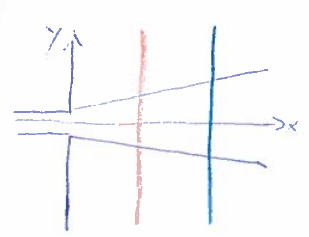
\includegraphics[width=.4\textwidth]{week5/momentum-flux}\\
    \caption{}
    \label{fig:momentum-flux}
\end{figure}

\begin{align}
\mathrm{momentum} & =\rho_0\Delta V\cdot v_x\\
&= \rho_0\Delta Av_x\Delta tv_x
\end{align}

Momentum flux:
\begin{equation}
\frac{\mathrm{momentum}}{\Delta A \Delta t} = \rho_0 v_x^2
\end{equation}

\noindent\makebox[\linewidth]{\rule{\textwidth}{0.5pt}}
\textbf{Proof of conservation of momentum flux}

If
\begin{equation}
\int_{-\infty}^\infty \rho_0v_x^2(x)dy=\mathrm{constant}
\end{equation}
then
\begin{equation}
\diff{}{x}\int_{-\infty}^\infty \rho_0v_x^2(x)dy=0
\end{equation}

\begin{align}
\diff{}{x}\int_{-\infty}^\infty \rho_0v_x^2(x)dy &= 2\rho_0\int_
{-\infty}^\infty\left(v_x\pdiff{v_x}{x}\right)dy \\
&= 2\mu\pdiff{v_x}{y}\biggm\vert_{-\infty}^\infty-2\rho_0\int_{-\infty}^\infty v_y\pdiff{v_x}{y}dy \\
&=-2\rho_0v_xv_y\biggm\vert_{-\infty}^\infty + 2\rho_0 \int_{-\infty}^\infty\pdiff{v_y}{y}dy \\
&= -2\rho_0\int_{-\infty}^\infty v_x\pdiff{v_x}{x}dy\\
&= 0
\end{align}
\noindent\makebox[\linewidth]{\rule{\textwidth}{0.5pt}}

\begin{align}
\int_{-\infty}^\infty\rho_0v_x^2dy &= \rho_0\int_{-\infty}^\infty v_\mathrm{max}^2(x)g^2\left(\frac{y}{\delta(x)}\right)dy\\
&= \rho_0v_\mathrm{max}^2(x)\delta(x)\int_{-\infty}^\infty g^2(z)dz\\
&\require \mathrm{constant}
\end{align}

\begin{align}
v_\mathrm{max}^2(x)\delta(x)&=\mathrm{constant}\\
c_1^2x^{2m}c_2x^n &= \mathrm{constant}\\
2m+n&0
\end{align}

\begin{align}
m+2n=1\ &,\qquad 2m+n=0 \\
\leadsto
m=-\frac{1}{3}\ &,\qquad n=\frac{2}{3}
\end{align}

\begin{align}
v_\mathrm{max}(x)&\sim\frac{1}{x^{1/3}}\\
\delta(x)&\sim x^{2/3}
\end{align}

\begin{framed}
\textbf{Remark:} negative jet flow

Wake behind a wind turbine can be modeled as a negative jet.

{\center
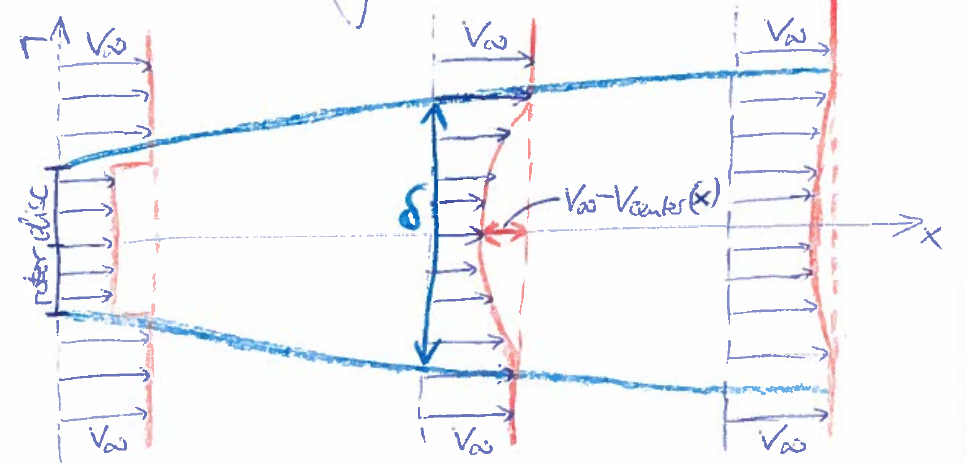
\includegraphics[width=.7\textwidth]{week5/negative-jet}\\
}

\begin{equation}
v_x(x,r) = v_\infty-v_\mathrm{center}(x)g\left(\frac{r}{\delta(x)}\right)
\end{equation}
\end{framed}
\section{Forces on a 2-dimensional body}
\begin{framed}
Ideal potential flows:
\begin{equation}
\vec{\nabla}\cdot\vec{u}=0=\vec{\nabla}\times\vec{u}\Rightarrow\vec{\nabla}\cdot\vec{\nabla}\phi = \left(\ppdiff{}{x}+\ppdiff{}{y}\right)\phi=0
\end{equation}
Where is the Euler equation? Do we need it?
\end{framed}
For an ideal potential flow the Euler equation
\begin{equation}
\rho \left(\pdiff{\vec{u}}{t}+\left(\vec{u}\cdot\vec{\nabla}\right)\vec{u}\right) = \rho \vec{f} - \vec{\nabla}p + \mu\left(\vec{\nabla}\cdot\vec{\nabla}\right)\vec{u}
\end{equation}
reduces to the Bernoulli equation:
\begin{equation}
\vec{\nabla}\left(\frac{\rho}{2}\vec{u}^2+p\right)=0.
\end{equation}
With the Bernoulli equation (leftover from the Euler equation) we can calculate the force on the "obstacle" (\fref{fig:2dim-body}) from the surrounding flow:
\begin{align}
\vec{F} &= \int_{S(u)}(-p(\vec{r}))d\vec{A} = -\int_{S(u)}\left(p_0-\frac{\rho}{2}\vec{u}^2(\vec{r})\right)d\vec{A} \\
&= \frac{\rho}{2}\int_{S(u)}\vec{u}^2(\vec{r})d\vec{A}\\
&= L\vec{e}_y +\underbrace{D\vec{e}_x}_{=0}.
\end{align}
$\vec{L}$ is the lift force and $\vec{D}$ is the drag force. The last term equals zero because there is no friction.

\begin{figure}[!h]
    \centering
    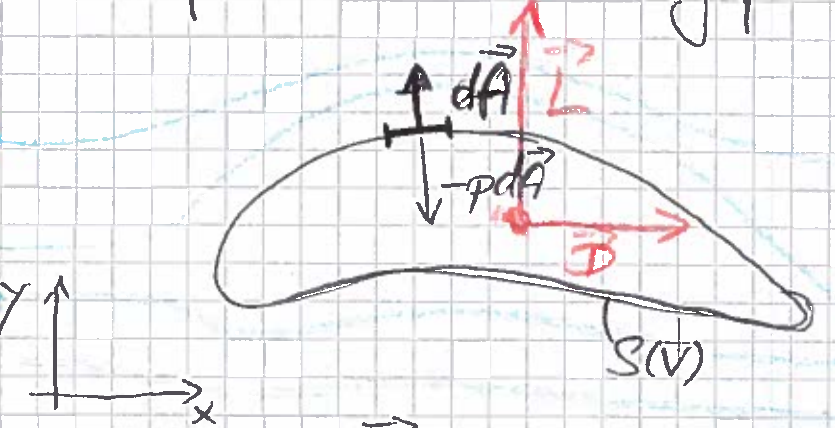
\includegraphics[width=.5\textwidth]{week4/2dim-body}\\
    \caption{Lift and drag forces.}
    \label{fig:2dim-body}
\end{figure}

\begin{figure}[!h]
    \centering
    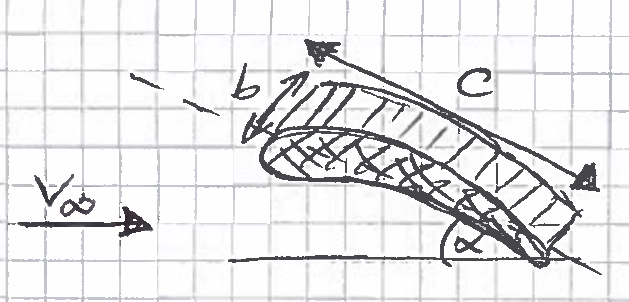
\includegraphics[width=.4\textwidth]{week4/generic-lift2}\\
    \caption{Angle of attack.}
    \label{fig:generic-lift2}
\end{figure}

Lift coefficient
\begin{equation}
C_L = \frac{L}{\frac{\rho}{2}v_\infty^2 b c}
\end{equation}
Drag coefficient (for the case that friction is non-zero):
\begin{equation}
C_D = \frac{D}{\frac{\rho}{2}v_\infty^2 b c}
\end{equation}

\begin{figure}[!h]
    \centering
    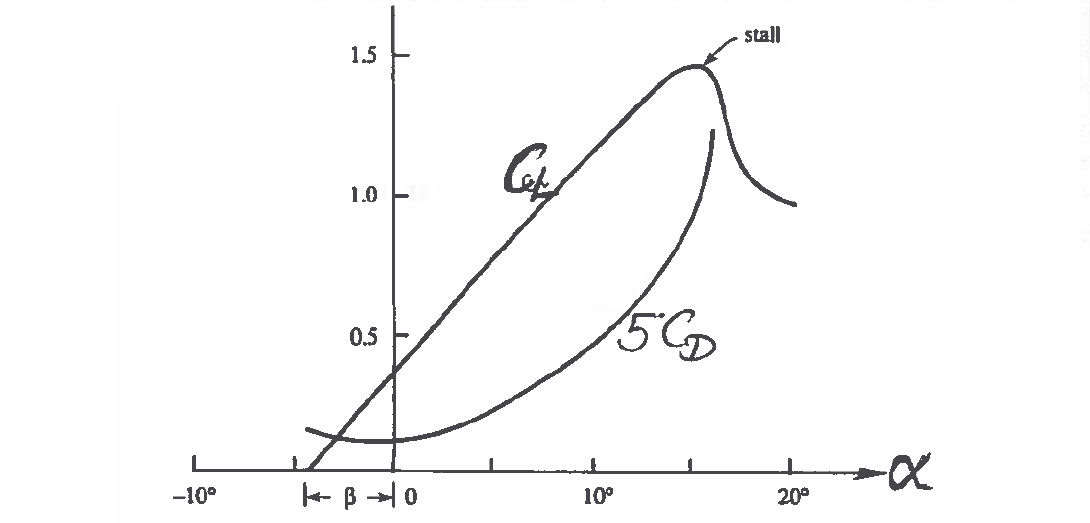
\includegraphics[width=.5\textwidth]{week4/generic-lift}\\
    \caption{Generic lift and drag coefficients vs. angle of attack. There is lift at $\alpha=0$ so the foil shape has nonzero camber. The drag increase is almost quadratic with increasing angle of attack.}
    \label{fig:generic-lift}
\end{figure}


\subsection{Turbine blade}
The lift force pulls the rotor blade of a wind turbine forward. See \fref{fig:turbine-blade}.
\begin{figure}[!h]
    \centering
    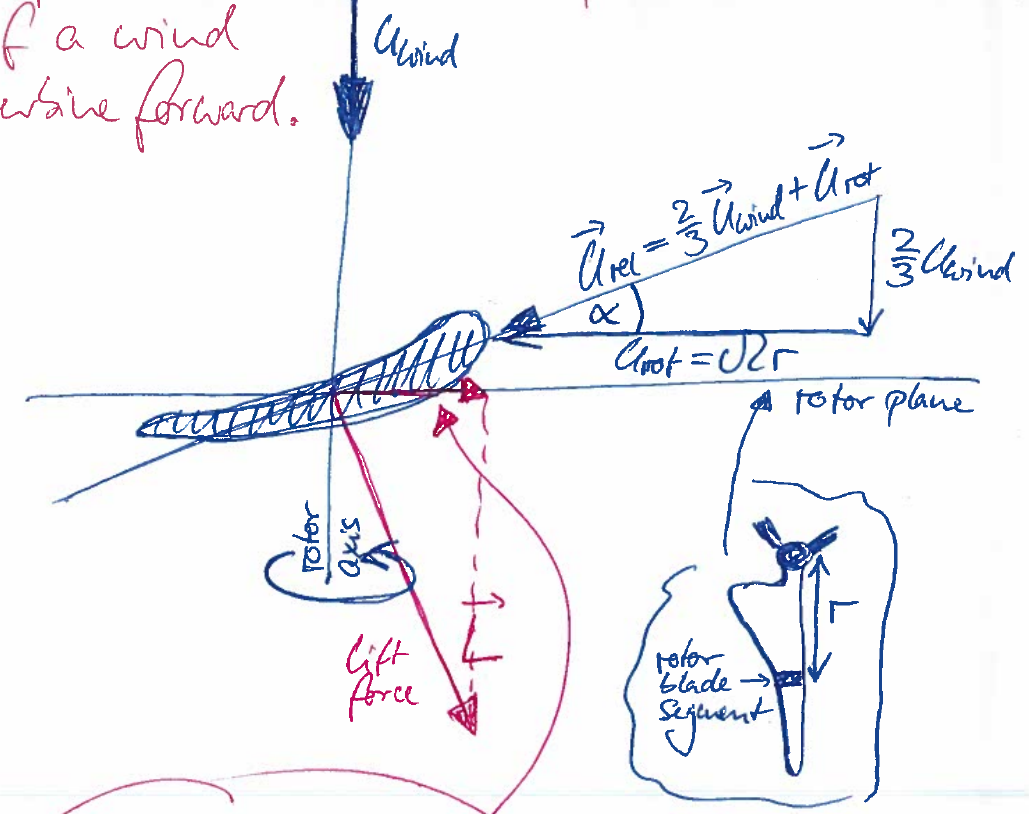
\includegraphics[width=.6\textwidth]{week4/turbine-blade}\\
    \caption{Lift and drag forces on the rotor blade of a wind turbine.}
    \label{fig:turbine-blade}
\end{figure}


\subsection[Sailing against the wind]{Sailing against the wind (KCD 14.9)}
People have sailed without the aid of an engine for thousands of years and have known
how to reach an upwind destination. Actually, it is not possible to sail exactly against the
wind, but it is possible to sail at $\approx$ 40-45$^\circ$ to the wind. \fref{fig:sailing-wind} shows
how this is made possible by the aerodynamic lift on the sail, which is a piece of stretched and stiffened
cloth. The wind speed is U, and the sailing speed is V, so that the apparent wind speed relative
to the boat is $U_r$. If the sail is properly oriented, this gives rise to a lift force perpendicular
to U$_\text{r}$ and a drag force parallel to U$_\text{r}$. The resultant force F can be resolved into a driving
component (thrust) along the motion of the boat and a lateral component. The driving
component performs work in moving the boat; most of this work goes into overcoming
the frictional drag and in generating the gravity waves that radiate outward from the hull.
The lateral component does not cause much sideways drift because of the shape of the
hull. It is clear that the thrust decreases as the angle $\theta$ decreases and normally vanishes
when $\theta$ is $\approx$ 40-45$^\circ$ . The energy for sailing comes from the wind field, which loses kinetic
energy after passing the sail.

\begin{figure}[!h]
    \centering
    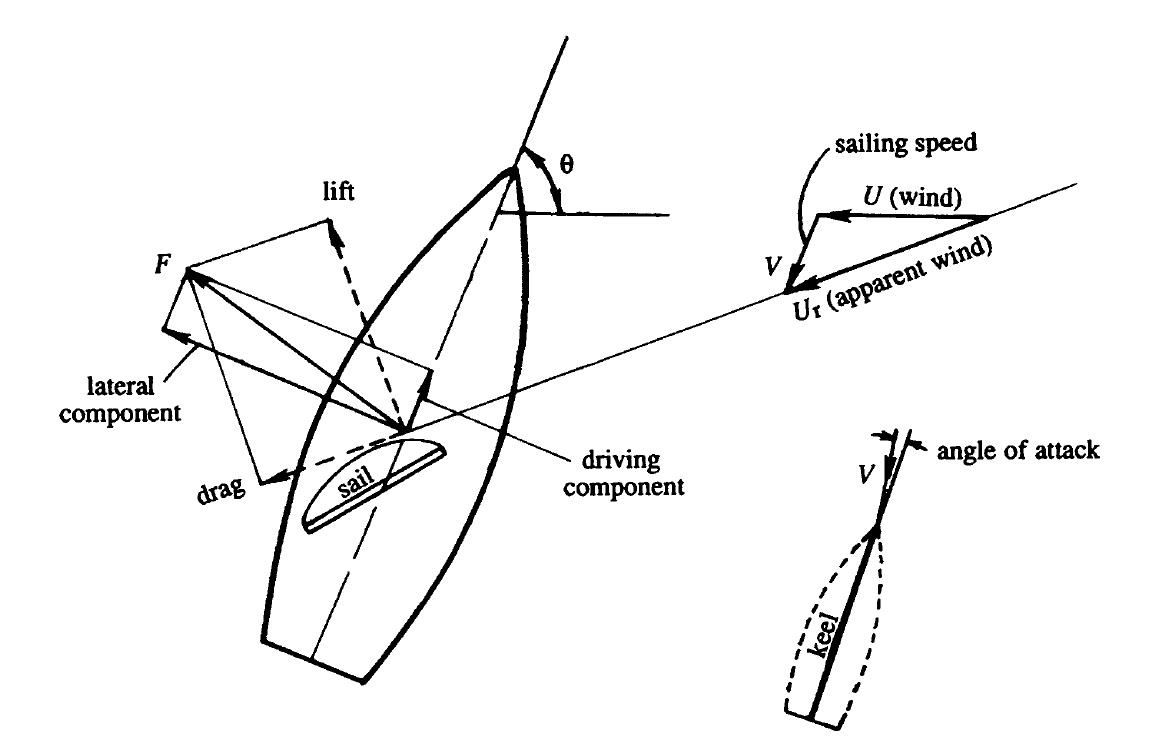
\includegraphics[width=.6\textwidth]{week4/sailing-wind}\\
    \caption{Principle of sailing against the wind. A small component of the sail’s lift pushes the boat forward at an angle $\theta$ < 90$^\circ$ to the wind. Thus by traversing a zig-zag course at angles $\pm\theta$, a sailboat can reach an upwind destination. A sailboat’s keel may make a contribution to its upwind progress too.}
    \label{fig:sailing-wind}
\end{figure}

\newpage
\subsection{Reynolds number}
Fluid around a cylinder can create several real flow patterns. See \fref{fig:reynolds-cylinder}.

\begin{figure}[p]
    \centering
    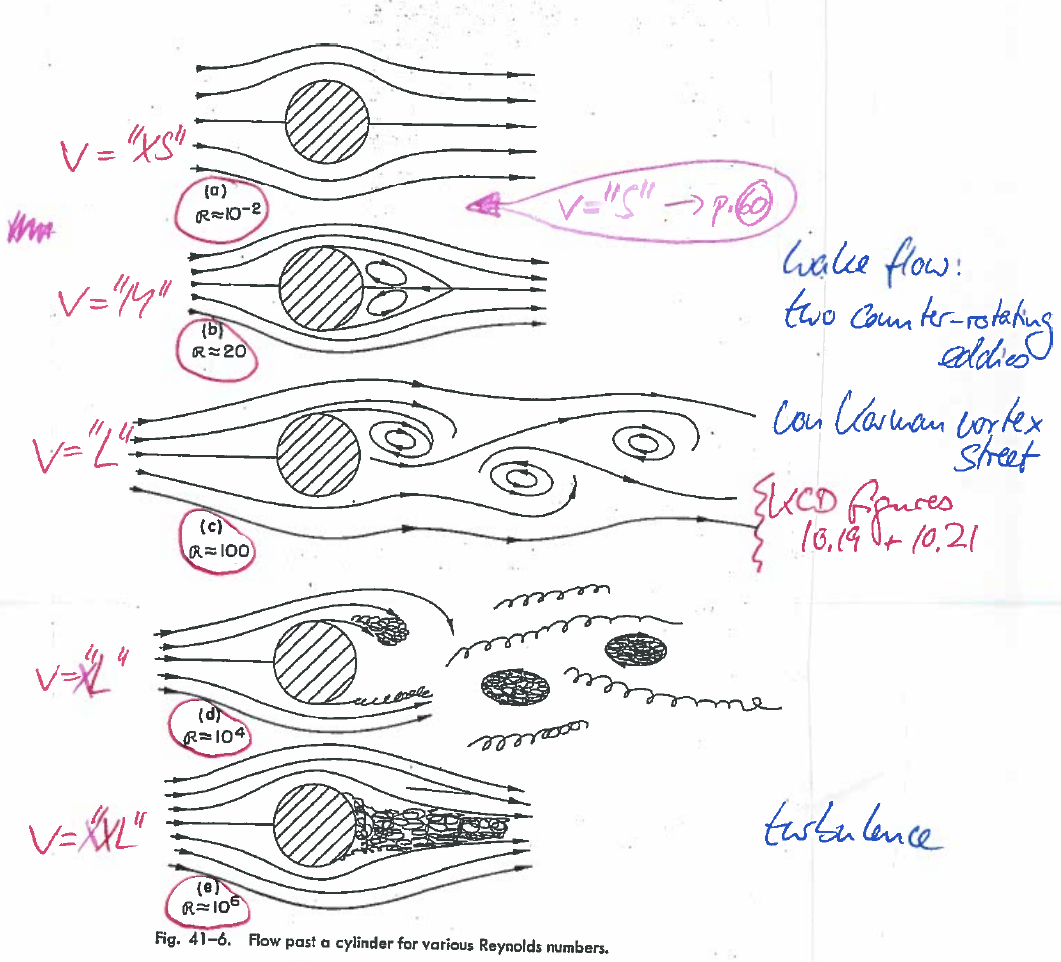
\includegraphics[width=\textwidth]{week4/reynolds-cylinder}\\
    \caption{Flow around a cylinder. From laminar to turbulent with increasing velocity.}
    \label{fig:reynolds-cylinder}
\end{figure}

\textbf{Questions:}
\begin{enumerate}
\item Why so many different flows?
\item What causes and characterizes them?
\end{enumerate}
Certainly friction, i.e. viscosity, will have something to do with it.

\begin{align}
0 &= \rho_0 \left[\pdiff{\vec{u}}{t}+\left(\vec{u}\cdot\vec{\nabla}\right)\vec{u}\right] + \vec{\nabla}p - \mu \left(\vec{\nabla}\cdot\vec{\nabla}\right) \vec{u} \\
&= \rho_0\left[\frac{U}{T}\pdiff{\vec{u}'}{t'}+\frac{U^2}{L}\left(\vec{u}'\cdot\vec{\nabla}'\right)\vec{u}'\right] + \frac{\rho_0 U^2}{L}\vec{\nabla}'p'-\mu\frac{U}{L^2}\left(\vec{\nabla}\cdot\vec{\nabla}\right)'\vec{u}' \\
&= \rho_0\frac{U^2}{L} \left\lbrace \pdiff{\vec{u}'}{t'}+\left(\vec{u}'\cdot\vec{\nabla}'\right)\vec{u}'+\vec{\nabla}'p'-\frac{\mu}{\rho_0 LV} \left(\vec{\nabla}\cdot\vec{\nabla}\right)'\vec{u}' \right\rbrace
\end{align}
where $L$ is the characteristic length, $U$ is the characteristic velocity, $T=L/U$ is the characteristic time, and $P=\rho_0U^2$ the characteristic pressure.

Reynolds number:
\begin{equation}
Re = \frac{\rho_0 L U}{\mu}
\end{equation}

\begin{framed}
\textbf{Remark:} law of similarity

If two flows have the same geometry (object) and the same Reynolds number, but a different absolute scale it means that the two flows are similar (identical, except for a scale transformation). Applications of this is wind tunnel experiments of air wings, wind turbine blades, cars, etc.
\end{framed}

The Reynolds number
\begin{equation}
Re = \frac{\rho_0 L U}{\mu} = \frac{\rho_0 U^2/L}{\mu U/L},
\end{equation}
is the inertia force density divided by the friction force density.

\begin{figure}[p]
    \centering
    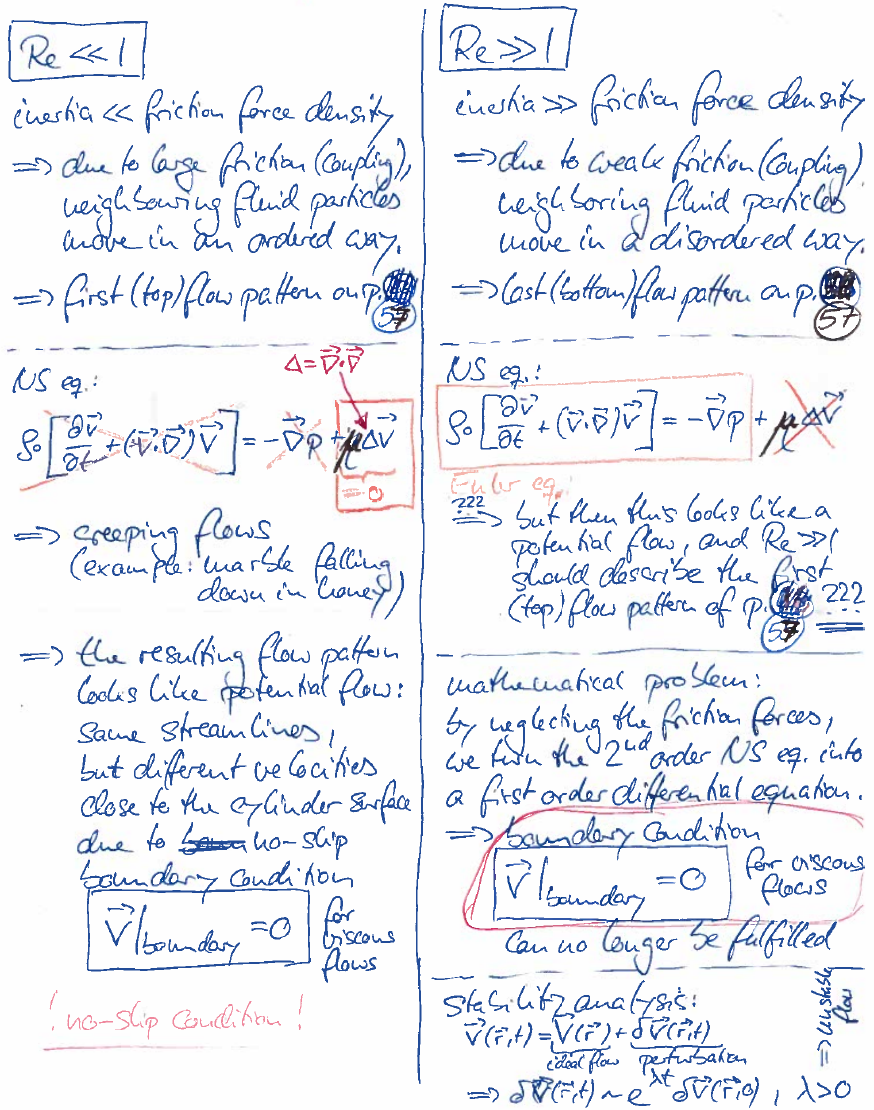
\includegraphics[width=\textwidth]{week4/reynolds-numbers}\\
    \caption{Extreme examples of Reynolds number.}
    \label{fig:reynolds-numbers}
\end{figure}

\begin{figure}[p]
    \centering
    \includegraphics[width=\textwidth]{week4/schematic-flows}\\
    \caption{Schematic real flow patterns around a cylinder with different Reynolds numbers.}
    \label{fig:schematic-flows}
\end{figure}


\newpage
\subsection{Viscous pipe flow}

\begin{figure}[ht]
    \centering
    \includegraphics[width=\textwidth]{week4/viscous-pipe-flow}\\
    \caption{Ideal and viscous pipe flow.}
    \label{fig:viscous-pipe-flow}
\end{figure}

Task: calculate velocity profile $u_z=u_z(r)$ for the viscous pipe flow.

Navier-Stokes equation
\begin{equation}
\rho_0\underbrace{\pdiff{\vec{u}}{t}}_{=0}+\rho_0\underbrace{\left(\vec{u}\cdot\vec{\nabla}\right)}_{=0}\vec{u} = \underbrace{\vec{f}_\mathrm{ext}}_{=0}-\vec{\nabla}p+\mu\left(\vec{\nabla}\cdot\vec{\nabla}\right)\vec{u}
\end{equation}
The second term on the left-hand side vanishes because of the incompressibility condition
\begin{equation}
0=\vec{\nabla}\cdot\vec{u}=\partial_xu_x+\partial_yu_y+\partial_zu_z = \partial_zu_z
\end{equation}
with $u_x=u_y=0$ and
\begin{equation}
\left(\vec{u}\cdot\vec{\nabla}\right)\vec{u} = u_z\partial_z
\begin{pmatrix}
0\\0\\u_z
\end{pmatrix} = 0.
\end{equation}
\begin{align}
\vec{\nabla}p = \mu\left(\ppdiff{}{x}+\ppdiff{}{y}\right)u_z\vec{e}_z\\
\leadsto
\left(\vec{\nabla}p\right)_x &= \left(\vec{\nabla}p\right)_y = 0 \\
\leadsto
p &= p(z)
\end{align}

\begin{align}
\mu\left(\partial_x^2+\partial_y^2\right) v_z(r) &= \frac{\mu}{r}\pdiff{}{r}\left(r\pdiff{u_z(r)}{r}\right) \\
&= \pdiff{p(z)}{z} \require \mathrm{constant}
\end{align}

\begin{align}
\pdiff{p(z)}{z}&=c \\
\leadsto
p(z) &= cz+d \\
&= \frac{p(z=L)-p(z=0)}{L}z+p(z=0)\\
&= -\frac{\Delta p}{L}z + p(z=0)
\end{align}

\begin{align}
\frac{\mu}{r}\pdiff{}{r}\left(r\pdiff{u_z(r)}{r}\right) &= c = -\frac{\Delta p}{L} \\
\leadsto
r\pdiff{u_z(r)}{r} &= -\frac{\Delta p}{\mu L}\frac{r^2}{2} + D_1 \\
\leadsto
u_z(r) &= -\frac{\Delta p}{4\mu L}r^2 + D_1 \ln r + D_ 2 \\
\end{align}
$D_1$ and $D_2$ are determined from the boudnary conditions $u_z(r=R)=0$ (no slip condition) and $|u_z(r=0)|<\infty$ (finiteness).
\begin{equation}
u_z(r) = \frac{\Delta p}{4\mu L}\left( R^2 - r^2\right)
\end{equation}

Fluid mass per time passing through pipe cross-section:
\begin{equation}
\diff{M}{t} = \int_0^R\rho_0 u_z(r)2\pi r dr = \frac{\pi\rho_0 R^4\Delta p}{8\mu L}
\end{equation}
This is the Hagen-Poiseuille law.
\begin{framed}
\textbf{Remark:} this law allows to determine the viscosity:
\begin{equation}
\left\lbrace \underbrace{\rho_0,R,L}_\mathrm{known} \quad,\quad \underbrace{\Delta p,\diff{M}{t}}_\mathrm{measured} \right\rbrace \Rightarrow \mu
\end{equation}
\end{framed}

\begin{framed}
\textbf{Remark:} "Ohm's Law"

\begin{align}
\Delta p = \Delta U \ &,\quad \diff{M}{t} = I\\
\leadsto
I &= \frac{\pi\rho_0 R^4}{8L\mu} \Delta U
\end{align}

{\center
\includegraphics[width=.4\textwidth]{week4/ohms-law}\\
}

\begin{equation}
R = R_0\cdot f(Re)
\end{equation}
with
\begin{equation}
f(Re\rightarrow0)=1.
\end{equation}
Turbulence increases pipe resistance. This is important for the operation of oil and gas pipelines.
\end{framed}



\newpage
\subsection{Boundary layers}

\begin{figure}[ht]
    \centering
    \includegraphics[width=\textwidth]{week4/boundary-layers}\\
    \caption{Example of boundary layer for flow around a cylinder.}
    \label{fig:boundary-layers}
\end{figure}

Idea of boundary layer theory:
\begin{enumerate}
\item within the boundary layer the velocity increases from zero to the ideal flow velocity
\item inside the boundary layer we use the Navier-Stokes equation (with friction)
\item outside the boundary layer we use the Euler equation without friction i.e. ideal potential flow
\item at the boundary surface we match the inside solution with the outside solution
\end{enumerate}

Derivation of the (laminar) boundary layer equations. Approximation to the Navier-Stokes equation inside the boundary layer. See \fref{fig:laminar-boundary}.

\begin{figure}[ht]
    \centering
    \includegraphics[width=.7\textwidth]{week4/laminar-boundary}\\
    \caption{Laminar boundary layer.}
    \label{fig:laminar-boundary}
\end{figure}

In the following we determine $\delta = \delta(x)$ (\fref{fig:laminar-boundary}) without solving the Navier-Stokes equation.

Incompressible flow:
\begin{align}
\vec{\nabla}\cdot\vec{u} = \pdiff{u_x}{x} + \pdiff{u_y}{y} &= 0 \\
\leadsto
\mathcal{O} \left(\frac{u_\infty}{L}\right) + \mathcal{O} \left(\frac{u_y}{\delta}\right) &= 0\\
\leadsto
\mathcal{O}(u_y) &= \delta\frac{u_\infty}{L} = \frac{\delta}{L}u_\infty
\end{align}

Navier-Stokes equation (x-component):
\begin{equation}
u_x\pdiff{u_x}{x} + u_y\pdiff{u_x}{y} = -\frac{1}{\rho_0}\pdiff{p}{x} + \frac{\mu}{\rho_0}\ppdiff{u_x}{x} + \frac{\mu}{\rho_0}\ppdiff{u_x}{y}
\end{equation}
\begin{equation}
\mathcal{O} \left(\frac{u_\infty^2}{L}\right) \require \mathcal{O} \left(\frac{\mu}{\rho_0}\frac{u_\infty}{\delta^2}\right)
\end{equation}

\begin{equation}
\left(\frac{\delta}{L}\right)^2 \sim \frac{\mu}{\rho_0 L u_\infty} = \frac{1}{Re}
\end{equation}
The larger the Reynolds number, the thinner the boundary layer. This holds for $Re \leq \SI{1e5}{}-\SI{1e6}{}$, above that the boundary layer becomes turbulent, and is no longer laminar.

\begin{equation}
\delta(x) \sim \sqrt{\frac{\mu x}{\rho_0 u_\infty}}
\end{equation}

Navier-Stokes equation (y-component):
\begin{equation}
u_x\pdiff{u_y}{x} + u_y\pdiff{u_y}{y} = -\frac{1}{\rho_0}\pdiff{p}{y} + \frac{\mu}{\rho_0}\ppdiff{u_y}{x} + \frac{\mu}{\rho_0}\ppdiff{u_y}{y}
\end{equation}
Ther first term on the right-hand side is the only large term. All other terms are neglected, which leads to
\begin{equation}
\pdiff{p}{y} = 0 \Rightarrow p = p(x)
\end{equation}

\begin{framed}
\textbf{Prandtl equations:} laminar boundary layer equations
\begin{align}
u_x\pdiff{u_x}{x}+u_y\pdiff{u_x}{y} &= -\frac{1}{\rho_0}\pdiff{p(x)}{x}+\frac{\mu}{\rho_0}\ppdiff{u_x}{y} \\
\pdiff{u_x}{x}+\pdiff{u_y}{y}&=0
\end{align}
\end{framed}

\textbf{Example:} Solution of Prandtl equations for laminar boundary flow around semi-infinite plate

\begin{equation}
p=p(x) \Rightarrow p(x)|_\mathrm{inside} = p(x)|_\mathrm{outside}
\end{equation}

Outside boundary layer:
\begin{align}
u_x|_\mathrm{outside} &= u_x = u_\infty = \mathrm{constant} \\
u_y|_\mathrm{outside} &= 0
\end{align}

Bernoulli equation:
\begin{align}
p(x) + \frac{\rho_0}{2}u_x^2 &= \mathrm{constant}\\
\leadsto
p(x) &= \mathrm{constant} \\
\leadsto
\pdiff{p(x)}{x} &= 0
\end{align}
Prandtl equations inside boundary layer:
\begin{align}
u_x\partial_xu_x+u_y\partial_yu_y &= \frac{\mu}{\rho_0}\partial_y^2u_x\\
\partial_xu_x+\partial_yu_y &= 0
\end{align}

\textbf{Solution:} similarity ansatz.
\begin{equation}
u_x(x,y) = u_\infty g\left(\frac{y}{\delta(x)}\right)
\end{equation}
Except for a rescaling with $\delta(x)$ the velocity $u_x(x,y)$ looks like the same for all $x$.
\begin{figure}[ht]
    \centering
    \includegraphics[width=.7\textwidth]{week4/boundary-ansatz}\\
    \caption{Similarity ansatz for the laminar boundary layer.}
    \label{fig:boundary-ansatz}
\end{figure}


\textbf{Question:} does the similarity ansatz work?
\begin{align}
\pdiff{u_x}{x}+\pdiff{u_y}{y} &= 0 \\
\leadsto
u_x = \pdiff{\psi}{y} \ &, \quad u_y = -\pdiff{\psi}{x}
\end{align}

\begin{equation}
\psi(x,y) = u_\infty\delta(x)f\left(\frac{y}{\delta(x)}\right)
\end{equation}

\begin{align}
u_x=\pdiff{\psi}{y} &= u_\infty\delta(x)\diff{f(z)}{z}\diff{z}{y} \\
&= u_\infty \delta(x) \diff{f(z)}{z}\frac{1}{\delta(x)}\\
&= u_\infty \diff{f(z)}{z} \\
&\require u_\infty g(z)
\end{align}

\begin{equation}
f' = \diff{f(z)}{z}g(z)
\end{equation}

\begin{align}
u_y &= -\pdiff{\psi}{x} \\
&=  -u_\infty\diff{\delta(x)}{x}f(z) - u_\infty \delta(x)\diff{f(z)}{z}\diff{z}{x}\\
&= u_\infty \left[-f + \frac{y f'}{\delta}\right] \diff{\delta(x)}{x}
\end{align}

\begin{align}
\pdiff{u_x}{x} &= \left(u_\infty f''\right)\left(\frac{-y}{\delta^2}\right)\diff{\delta(x)}{x} = -\frac{u_\infty y f''}{\delta^2}\diff{\delta(x)}{x} \\
\pdiff{u_x}{y} &= (u_\infty f'') \frac{1}{\delta} = \frac{u_\infty f''}{\delta} \\
\pdiff{u_x}{y} &= \frac{u_\infty f''}{\delta^2}
\end{align}

\begin{align}
\begin{split}
u_x\pdiff{u_x}{x} + u_y\pdiff{u_x}{y} - \frac{\mu}{\rho_0}\ppdiff{u_x}{y} &=
-(u_\infty f') \left(\frac{u_\infty y f''}{\delta^2} \diff{\delta(x)}{x}\right) \\
&\hspace{5mm} + \left(u_\infty\left[-f+\frac{yf'}{\delta}\right]\diff{\delta(x)}{x}\right) \left(\frac{u_\infty f''}{\delta}\right) \\
&\hspace{5mm} -\frac{\mu}{\rho_0} \left(\frac{u_\infty f''}{\delta^2}\right)
\end{split} \\
&= -\frac{u_\infty^2}{\delta}\diff{\delta}{x} ff'' - \frac{\mu}{\rho_0} \frac{u_\infty}{\delta^2}f'''\\
&= 0
\end{align}

\begin{equation}
\frac{\rho_0 u_\infty}{\mu} \delta(x) \diff{\delta(x)}{x} = -\frac{f'''(z)}{f(z)f''(z)} \require c_1^2
\end{equation}

\begin{equation}
\delta\diff{\delta}{x} = \frac{1}{2}\diff{\delta^2}{x} = c_1^2\frac{\mu}{\rho_0u_\infty}\\
\end{equation}

\begin{equation}
\delta^2 = 2c_1^2 \frac{\mu}{\rho_0u_\infty}x + c_2
\end{equation}
$c_2=0$ since $\delta(x=0)=0$.

\begin{equation}
\delta(x) = c_1\sqrt{\frac{2\mu}{\rho_0u_\infty}x}
\end{equation}

\begin{equation}
\delta(x)=\sqrt{\frac{\mu}{\rho_0u_\infty}x}
\end{equation}
Freedom of choice $c_1=\frac{1}{\sqrt{2}}$ because of arbitrary definition of $\delta$; for example, $u_x(y=\delta)=0.99u_\infty$ or $u_x(x=\delta)=0.95u_\infty$.

This is the same result as the order of magnitude calculation when we calculated the x-component of the Navier-stokes equation earlier in this section.

\begin{equation}
f'''(z) +\frac{1}{2} f(z)f''(z) = 0
\end{equation}

\begin{equation}
f(z)\ddiff{f(z)}{z}+2\dddiff{f(z)}{z}=0
\end{equation}
This is Blasius' equation. It is a special case of the more general Falker-Skan equation. The Blasius equation can only be solved numerically. The boundary conditions for the solutions are:
\begin{align}
u_x(y=0)=0&\Rightarrow f'(0)=0, \\
u_y(y=0)=0&\Rightarrow f(0)=0, \\
u_x(y=\infty)=u_\infty&\Rightarrow f'(\infty)=1.
\end{align}
The solution is sketched in \fref{fig:blasius}.
\begin{figure}[!h]
    \centering
    \includegraphics[width=.8\textwidth]{week4/blasius}\\
    \caption{Solution to the Blasius equation.}
    \label{fig:blasius}
\end{figure}


\subsection{Separation of boundary layers}
Boundary condition at the wall:
\begin{equation}
v_x(x,y=0) = v_y(x,y=0)=0
\end{equation}

Prandtl equation (with pressure)
\begin{equation}
v_x\pdiff{v_x}{x}+v_y\pdiff{v_x}{y} = -\frac{1}{\rho_0}\pdiff{p}{x}+\frac{\mu}{\rho_0}\ppdiff{v_x}{y}
\end{equation}
If we are very close to the wall, the two terms on the left side equal zero. We then have
\begin{equation}
\pdiff{p(x,y=0)}{x}=\mu\ppdiff{v_x(x,y=0)}{y}
\end{equation}

\begin{figure}[!h]
    \centering
    \includegraphics[width=.9\textwidth]{week5/wall-boundary}\\
    \caption{Shape of the boundary layer for different pressure profiles.}
    \label{fig:wall-boundary}
\end{figure}

\begin{figure}[!h]
    \centering
    \includegraphics[width=.5\textwidth]{week5/detachment-point}\\
    \caption{Detachment point of the boundary layer.}
    \label{fig:detachment-point}
\end{figure}

\newpage
\textbf{Example:} flow around cylinder

\begin{figure}[!h]
    \centering
    \includegraphics[width=.8\textwidth]{week5/cylinder-flow}\\
    \caption{Separation of boundary layer and detachment point for flow around a cylinder.}
    \label{fig:cylinder-flow}
\end{figure}

The detachment point is at the separation of the boundary layer. When $v\approx0$ there is no kinetic energy to run against the pressure gradient.

\begin{framed}
\textbf{Remark:} separation of boundary layers is a big issue in mechanical engineering; for example: design of airfoils, wind-turbine blades etc.
{\center
\includegraphics[width=.4\textwidth]{week5/detachment-eddies}\\
}
In case of separation the lift decreases, which can lead to airplane crash. It would also lead to a substantial rise in the overall drag (more friction). This would require more engine power and therefore more fuel for an airplane. For a wind turbine it would means less power generation.

Engineer's dream: construct airfoils without turbulent wake, with e.g. shark skin or fish scales.
\end{framed}


\subsection{Solution of Prandtl equations for free boundary layers}
\fref{fig:2d-laminar-jet} shows a 2-dimensional laminar jet flow generated from a flow through a long slit streaming into a resting fluid.
\begin{figure}[!h]
    \centering
    \includegraphics[width=.6\textwidth]{week5/2d-laminar-jet}\\
    \caption{2-dimensional laminar jet flow.}
    \label{fig:2d-laminar-jet}
\end{figure}

We use the Prandtl equations with the similarity ansatz:
\begin{equation}
v_x(x,y)=v_\mathrm{max}(x)g\left(\frac{y}{\delta(x)}\right)
\end{equation}

\begin{equation}
\pdiff{v_x}{x}+\pdiff{v_y}{y}=0 \Rightarrow v_x=\pdiff{\psi}{y},\quad v_y=-\pdiff{\psi}{x}
\end{equation}

\begin{equation}
\psi = v_\mathrm{max}(x)\delta(x)f\left(\frac{y}{\delta(x)}\right)
\end{equation}

\begin{equation}
\pdiff{\psi}{y}=v_\mathrm{max}\delta f'\frac{1}{\delta}=v_\mathrm{max}f'=v_\mathrm{max}g=v_x
\end{equation}

\begin{equation}
v_y=-\pdiff{\psi}{x}=-v'_\mathrm{max}\delta f-v_\mathrm{max}\delta'f-v_\mathrm{max}\delta f'\frac{(-y)\delta'}{\delta^2}
\end{equation}

\begin{align}
\partial_xv_x &= v'_\mathrm{max}f'+v_\mathrm{max}f''\frac{(-y)\delta'}{\delta^2} \\
\partial_yv_x &= v_\mathrm{max} f''\frac{1}{\delta}\\
\partial^2_yv_x &= \frac{v_\mathrm{max}}{\delta^2}f'''
\end{align}
Insertion into Prandtl's equation with $p(x)=\text{constant}$:
\begin{align}
\begin{split}
v_x\partial_x v_x+v_y\partial_yv_x-\frac{\mu}{\rho_0}\partial^2_yv_x &= v_\mathrm{max}f'\left\lbrace v'_\mathrm{max}f' - v_\mathrm{max}\frac{y\delta'}{\delta^2}f''\right\rbrace \\
&\hspace{5mm}-\left\lbrace v'_\mathrm{max}\delta f + v_\mathrm{max}\delta'f-v_\mathrm{max}\frac{y\delta'}{\delta}f'\right\rbrace v_\mathrm{max}\frac{1}{\delta}f'' \\
&\hspace{5mm}-\frac{\mu}{\rho_0^2} \frac{v_\mathrm{max}}{\delta^2}f'''
\end{split}\\
\begin{split}
&= v_\mathrm{max}v'_\mathrm{max}f'^2-v_\mathrm{max}v'_\mathrm{max}ff''-v_\mathrm{max}^2\frac{\delta'}{\delta}ff'' \\
&\hspace{5mm}-\frac{\mu}{\rho_0}\frac{v_\mathrm{max}}{\delta^2}f'''\label{eq:free-boundary}
\end{split} \\
&\require0 \label{eq:prandtl}
\end{align}
All four terms in \eqref{eq:free-boundary} have the form $\alpha_i(x)\beta_i(x)$ for $(i=1,...,4)$. The sum of these four terms has to be zero. This means that $\alpha_1(x)\sim\alpha_2(x)\sim\alpha_3(x)\sim\alpha_4(x)$.

Ansatz:
\begin{align}
v_\mathrm{max}(x) &= c_1x^m\\
\delta(x) &= c_2 x^n
\end{align}

\begin{framed}
\textbf{Remark:} we expect $m<0$ (decreasing velocity with penetration depth) and $n>0$ (increasing thickness of jet with penetration depth).
\end{framed}

Sum of the 4 terms:
\begin{equation}
c_1^2mx^{2m-1}(f'^2-ff'')-c_1^2x^{2m}\frac{n}{x}ff'' - \frac{\mu}{\rho_0}\frac{c_1}{c_2^2}\frac{x^m}{x^{2n}}f'''=0
\end{equation}

\begin{framed}
\begin{equation}
2m-1 = m-2n
\end{equation}
\begin{equation}
m(f'^2-ff'')-nff''-\frac{\mu}{\rho_0}\frac{1}{c_1c_2^2}f'''=0
\end{equation}
\end{framed}

This differential equation determines the velocity profile
\begin{equation}
g\left(\frac{y}{\delta(x)}\right)=f'\left(\frac{y}{\delta(x)}\right)
\end{equation}
of the jet. We are not going to solve this, but we want to know $m$ and $n$, because they determine $v_\mathrm{max}(x)$ and $\delta(x)$. We need a second equation for $m$ and $n$.

\textbf{Second equation:} conservation of momentum flux.
Momentum flux through the red plane in \fref{fig:momentum-flux} is identical to the momentum flux through the blue plane. This means that the integrated momentum flux does not depend on $x$.
\begin{figure}[!h]
    \centering
    \includegraphics[width=.4\textwidth]{week5/momentum-flux}\\
    \caption{Momentum flux for 2-dimensional laminar jet flow.}
    \label{fig:momentum-flux}
\end{figure}

\begin{align}
\mathrm{momentum} & =\rho_0\Delta V\cdot v_x\\
&= \rho_0\Delta Av_x\Delta tv_x
\end{align}

Momentum flux:
\begin{equation}
\frac{\mathrm{momentum}}{\Delta A \Delta t} = \rho_0 v_x^2
\end{equation}

\begin{framed}
\textbf{Proof of conservation of momentum flux}

If
\begin{equation}
\int_{-\infty}^\infty \rho_0v_x^2(x)dy=\mathrm{constant}
\end{equation}
then
\begin{equation}
\diff{}{x}\int_{-\infty}^\infty \rho_0v_x^2(x)dy=0
\end{equation}

\begin{align}
\diff{}{x}\int_{-\infty}^\infty \rho_0v_x^2(x)dy &= 2\rho_0\int_{-\infty}^\infty\left(v_x\pdiff{v_x}{x}\right)dy \label{eq:a}\\
&= 2\mu\pdiff{v_x}{y}\biggm\vert_{-\infty}^\infty-2\rho_0\int_{-\infty}^\infty v_y\pdiff{v_x}{y}dy \label{eq:b}\\
&=-2\rho_0v_xv_y\biggm\vert_{-\infty}^\infty + 2\rho_0 \int_{-\infty}^\infty\pdiff{v_y}{y}dy \label{eq:c}\\
&= -2\rho_0\int_{-\infty}^\infty v_x\pdiff{v_x}{x}dy \label{eq:d}\\
&= 0
\end{align}
Prandtl's equation \eqref{eq:prandtl} has been inserted into \eqref{eq:a} to obtain \eqref{eq:b}. The first term in \eqref{eq:b} is zero because $v_x(y)=\text{constant}$ for $y\rightarrow\pm\infty$. Partial integration has been used to arrive at \eqref{eq:c}. The incompressibility condition $\partial_xv_x+\partial_yv_y$ has been used to get \eqref{eq:d}. Since \eqref{eq:d} is equal to \eqref{eq:a} the integral has to be zero.
\end{framed}

\begin{align}
\int_{-\infty}^\infty\rho_0v_x^2dy &= \rho_0\int_{-\infty}^\infty v_\mathrm{max}^2(x)g^2\left(\frac{y}{\delta(x)}\right)dy\\
&= \rho_0v_\mathrm{max}^2(x)\delta(x)\int_{-\infty}^\infty g^2(z)dz\\
&\require \mathrm{constant}
\end{align}

\begin{align}
v_\mathrm{max}^2(x)\delta(x)&=\mathrm{constant}\\
c_1^2x^{2m}c_2x^n &= \mathrm{constant}\\
2m+n &= 0
\end{align}

\begin{align}
m+2n=1\ &,\qquad 2m+n=0 \\
\leadsto
m=-\frac{1}{3}\ &,\qquad n=\frac{2}{3}
\end{align}

\begin{align}
v_\mathrm{max}(x)&\sim\frac{1}{x^{1/3}}\\
\delta(x)&\sim x^{2/3}
\end{align}

\begin{framed}
\textbf{Remark:} negative jet flow

Wake behind a wind turbine can be modeled as a negative jet.

{\center
\includegraphics[width=.7\textwidth]{week5/negative-jet}\\
}

\begin{equation}
v_x(x,r) = v_\infty-v_\mathrm{center}(x)g\left(\frac{r}{\delta(x)}\right)
\end{equation}
\end{framed}
\section{Instabilities (89-105)}

\textbf{Motivation:} Navier-Stokes equation in non-dimensional units with no external forces:
\begin{equation}
\pdiff{\vec{v}}{t}+\left(\vec{v}\cdot\vec{\nabla}\right)\vec{v} = -\vec{\nabla}p+\frac{1}{Re}\vec{\nabla}^2\vec{v}
\end{equation}

Reynolds number:
\begin{equation}
Re = \frac{\rho LV}{\mu}=\frac{\rho V^2/L}{\mu V/L^2}=\frac{\mathrm{inertia\ force\ density}}{\mathrm{friction\ force\ density}}
\end{equation}
As the Reynolds number increases, a stable flow becomes unstable, and a new stable flow emerges.

\textbf{Big question:} when does a stable flow become unstable?

Answer: linear stability analysis

\begin{figure}[h]
    \centering
    \includegraphics[width=.8\textwidth]{week7/stable-unstable}\\
    \caption{}
    \label{fig:stable-unstable}
\end{figure}


\begin{figure}[p]
    \centering
    \includegraphics[width=\textwidth]{week7/reynolds-number}\\
    \caption{}
    \label{fig:reynolds-number}
\end{figure}


\textbf{Sketch of linear stability analysis}

Simplifying assumptions: stable flows are steady (stationary)
\begin{equation}
\vec{v}(\vec{r},t)=\vec{U}(\vec{r})\ ,\quad p(\vec{r},t)=P(\vec{r})
\end{equation}

Introduce perturbations
\begin{align}
\vec{v}(\vec{r},t)&=\vec{U}(\vec{r})+\vec{u}(\vec{r},t)\\
p(\vec{r},t)&=P(\vec{r})+\tilde{p}(\vec{r},t)
\end{align}

\begin{equation}
\pdiff{(\vec{U}+\vec{u})}{t}+\left[(\vec{U}+\vec{u})\cdot\vec{\nabla}\right](\vec{U}+\vec{u}) = -\vec{\nabla}(P+\tilde{p})+\frac{1}{Re}\left(\vec{\nabla}\cdot\vec\nabla\right)(\vec{U}+\vec{u})
\end{equation}

\begin{align}
\begin{split}
\pdiff{\vec{U}}{t}+(\vec{U}+\vec{\nabla})\vec{U}+\pdiff{\vec{u}}{t}+(\vec{U}+\vec{\nabla})\vec{u}& \\
+ (\vec{u}+\vec{\nabla})\vec{U} + (\vec{u}+\vec{\nabla})\vec{u} &= -\vec{\nabla}P\frac{1}{Re}\left(\vec{\nabla}\cdot\vec\nabla\right)\vec{U} \\
&\hspace{5mm}-\vec{\nabla}\tilde{p}+\frac{1}{Re}\left(\vec{\nabla}\cdot\vec\nabla\right)\vec{u}
\end{split}
\end{align}


\begin{equation}
\pdiff{\vec{u}}{t}+\left(\vec{U}\cdot\vec\nabla\right)\vec{u}+\left(\vec{u}\cdot\vec\nabla\right)\vec{U} = -\vec{\nabla}\tilde{p}+\frac{1}{Re}\left(\vec{\nabla}\cdot\vec\nabla\right)\vec{u}
\end{equation}

\begin{equation}
\vec{\nabla\cdot\vec{u}}=0
\end{equation}

\begin{equation}
\vec{u}(\vec{r},t)=e^{\lambda t}\vec{u}(\vec{r,0})
\end{equation}

\begin{equation}
\lambda\vec{u}(\vec{r},t) = \frac{1}{Re}\left(\vec{\nabla}\cdot\vec\nabla\right)\vec{u}(\vec{r},t)-\vec{\nabla}\tilde{p}-\left(\vec{U}\cdot\vec\nabla\right)\vec{u}(\vec{r},t)-\left(\vec{u}\cdot\vec\nabla\right)\vec{U}(\vec{r},t)
\end{equation}

\begin{equation}
\vec{\nabla}\cdot\vec{u}(\vec{r},t) = 0
\end{equation}
This is an eigenvalue equation.

\begin{equation}
\lambda = \lambda(Re, \vec{U})
\end{equation}
depends on $Re$ and $\vec{U}(\vec{r})$ and $\vec{u}(\vec{r},0)$.

If $\lambda<0$: $\vec{U}(\vec{r})$ is stable and the perturbations damps out. If $\lambda>0$: $\vec{U}(\vec{r})$ is unstable and the perturbation grows.


\textbf{Linear stability analysis of the poor man's Navier-Stokes equation}

\begin{equation}
\pdiff{\vec{v}}{t} = -\left[\left(\vec{v}\cdot\vec{\nabla}\right)\vec{v}+\vec{\nabla}p\right]+\frac{1}{Re}\vec{\nabla}^2\vec{v} + \vec{f}
\end{equation}

"analogy"
\begin{equation}
v_{t+1} - v_t = -2v_t^2 - v_t + 1
\end{equation}

Oversimplification: discrete time steps $\Delta t=1$, no spatial structure, no vector.

\begin{equation}
v_{t+1}=1-2v_t^2\ ,\qquad -1\leq v_t\leq1
\end{equation}

substitution
\begin{align}
v_t&=2x_t-1\\
\leadsto
x_{t+1}&=4x_t(1-x_t)\ ,\quad 0\leq x_t\leq 1
\end{align}

generalization
\begin{equation}
x_{t+1}=rx_t(1-x_t)\ ,\quad 0\leq r\leq 4
\end{equation}
This is the famous logistic (quadratic) map of deterministic chaos.

The order parameter $r$ is analogous to $Re$: different dynamic (temporal) patterns for different $r$.

As $r$ increases an "old pattern" becomes unstable, and a "new pattern" emerges.

\begin{figure}[h]
    \centering
    \includegraphics[width=\textwidth]{week7/graphical-solution}\\
    \caption{}
    \label{fig:graphical-solution}
\end{figure}

\begin{framed}
\textbf{Linear stability analysis}
\begin{align}
x_{t+1}&=x^*+\delta x_{t+1} = f(x_t)=f(x^*+\delta x_t)\\
&\approx f(x^*) + f'(x^*)\delta x_t 0 + \cdots
\end{align}
Perturbations are only kept up to first order (linearization). Quadratic and higher order terms are neglected.
\begin{equation}
\biggm\vert\frac{\delta x_{t+1}}{\delta x_{t}}\biggm\vert=|f'(x^*)|
\end{equation}
\begin{align}
|f'(x^*)|<1&:\quad |\delta x_t|=|f'(x^*)|^t|\delta x_0|=e^{\lambda t}|\delta x_0 \\
|f'(x^*)|>1&:\quad  |\delta x_t|=e^{\lambda t}|\delta(x_0)|
\end{align}
\end{framed}


\begin{align}
f(x) &= rx(1-z) \\
\leadsto
f'(x) &= r[(1-x)-x]=r(1-2x) \\
\leadsto
|f'(x^*=0)|&=r\\
\leadsto
x^* &= 0
\end{align}
Stable fixed point for $r<1$. Unstable fixed point for $r>1$.

\textbf{Question:} what happens for $r>1$?
\begin{figure}[h]
    \centering
    \includegraphics[width=\textwidth]{week7/linear-stability}\\
    \caption{}
    \label{fig:linear-stability}
\end{figure}

Fixed points:
\begin{align}
x^* &= f(x^*) = rx^*(1-x^*)\\
\leadsto
x_0^*=0\ &,\quad x_1^* = \frac{r-1}{r}
\end{align} 

Stability:
\begin{equation}
f'(x_0^*) = r>1
\end{equation}
which means that $x_0^*$ is an unstable fixed point.

\begin{equation}
|f'(x_1^*)|=\biggm\vert r\left(1-2\frac{r-1}{r}\right)\biggm\vert=|2-r|
\end{equation}

\begin{equation}
|f'(x_1^*)| < 1 \Rightarrow 1<r<4
\end{equation}
which means that $x_1^*$ is a stable fixed point.

\textbf{Question:} what happens for $r>3$?

\begin{figure}[p]
    \centering
    \includegraphics[width=\textwidth]{week7/linear-stability-2}\\
    \caption{}
    \label{fig:linear-stability-2}
\end{figure}

\begin{framed}
two cycle $(r_1=3<r<r_2=?)$: jumps between two values $x_1^*$ and $x_2^*$.

\begin{align}
x_2^*=f(x_1^*)\ &,\quad x_1^*=f(x_2^*) \\
\leadsto
x_2^* = f(f(x_2^*))\, &,\quad x_1^*=f(f(x_1^*))
\end{align}

\begin{align}
f^{(2)}(x) &= f(f(x)) = rf(x)(1-f(x))\\
&= r^2x(x-1)[1-rx(1-x)]
\end{align}

\begin{equation}
\biggm\vert\diff{f^{(2)}(x)}{x}\biggm\vert<1 \Rightarrow r_1=3<r<r_2=?
\end{equation}
stable two-cycle
\end{framed}

\begin{framed}
$r_2<r<r_3$ is a stable four-cycle
\begin{align}
f^{(4)}(x)&=f(f(f(f(x))))\\
\biggm\vert\diff{f^{(4)}(x)}{x}\bigg\vert&<1
\end{align}
\end{framed}
\begin{equation}
3<r\leq r_\infty = 3.57...
\end{equation}
2-cycle, 4-cycle, 8-cycle, ...

\begin{figure}[h]
    \centering
    \includegraphics[width=\textwidth]{week7/bifurcation}\\
    \caption{}
    \label{fig:bifurcation}
\end{figure}

\begin{equation}
3.57... \leq r \leq 4
\end{equation}
Mostly chaotic.

\newpage
\textbf{Question:} how can we characterize deterministic chaos?

Liapunov exponent:

\begin{figure}[h]
    \centering
    \includegraphics[width=\textwidth]{week7/liapunov}\\
    \caption{}
    \label{fig:liapunov}
\end{figure}

\begin{equation}
\delta x_0e^{n\lambda(x_0)}=|f^{(n)}(x_0+\delta x_0)-f^{(n)}(x_0)|
\end{equation}

\begin{align}
\lambda(x_0) &= \lim_{n\rightarrow\infty}\lim_{\delta x_0\rightarrow0}\frac{1}{n}\ln \biggm\vert \frac{f^{(n)}(x_0+\delta x_0-f^{(n)}(x_0)}{\delta x_0} \\
&= \lim_{n\rightarrow\infty}\frac{1}{n}\ln|(f^{(n)}(x_0))'|\\
&= \lim_{n\rightarrow\infty}\frac{1}{n}\ln|f'(x_{n-1})\cdot f'(x_{n-2})\cdot ... \cdot f'(x_{1})\cdot f'(x_{0})|
\end{align}

\begin{equation}
\lambda(x_0)=\lim_{n\rightarrow\infty}\frac{1}{n}\sum_{i=0}^{n-1}\ln|f'(x_i)|
\end{equation}

Attractive stable limit cycle (with period $T=m$)
\begin{equation}
\lambda(x_0)=\frac{1}{m}\sum_{i=0}^{m-1}\ln|f'(x_i^*)|<0
\end{equation}

Neighboring phase space trajectories with nearly identical initial conditions converge towards each other.

Deterministic chaos:
\begin{equation}
\lambda(x_0)>0
\end{equation}
neighboring trajectories diverge
\begin{figure}[h]
    \centering
    \includegraphics[width=.8\textwidth]{week7/chaos}\\
    \caption{}
    \label{fig:chaos}
\end{figure}

\textbf{Special case (of the logistic map):} $r=4$

Observation: $\lambda(x_0)>0$ leads to divergence of neighboring trajectories. All values $0\leq x_t\leq 1$ occur (as $t$ runs its course).

\textbf{Question:} what is the probability density for a specific x-value?

\begin{equation}
x_{t+1} = 4x_t(1-x_t)
\end{equation}
Substitution:
\begin{equation}
x_t=\frac{1}{2}[1-\cos(2\pi y_t)]
\end{equation}

\begin{align}
t_{t+1} &= \frac{1}{2}[1-\cos(2\pi y_{t+1})] = 4x_t(1-x_t) \\
&= \frac{4}{2}[1-\cos(2\pi y_{t})]\left[1-\frac{1}{2}+\frac{1}{2}\cos(2\pi y_t)\right]\\
&= [1-\cos(2\pi y_{t})][1+\cos(2\pi y_{t})]\\
&= 1-\cos^2(2\pi y_t \\
&=\frac{1}{2}+\frac{1}{2}[\sin^2(2\pi y_t)+\cos^2(2\pi y_t)]-\cos^2(2\pi y_t)\\
&= \frac{1}{2}+\frac{1}{2}[\sin^2(2\pi y_t)-\cos^2(2\pi y_t)]\\
&= \frac{1}{2}[1-\cos(4\pi y_t)]
\end{align}

Solution:
\begin{equation}
y_{t+1} = 2y_t\ ,\quad 0\leq y_t \leq 1
\end{equation}
\begin{equation}
y_t = 2^ty_0
\end{equation}

\begin{figure}[h]
    \centering
    \includegraphics[width=\textwidth]{week7/other-solution}\\
    \caption{}
    \label{fig:other-solution}
\end{figure}

\begin{framed}
Once again: sensitive dependence on initial conditions

\begin{equation}
y_0 = \alpha_12^{-1} + \alpha_22^{-2} + \alpha_32^{-3} + \dots = \sum_{i=1}^\infty\alpha_i2^{-i}
\end{equation}

\begin{align}
y_1 &= 2y_0 \\
&= \alpha_22^{-2} + \alpha_32^{-3} + \alpha_42^{-4}+\dots\\
&= \sum_{i=1+1}^\infty\alpha_{i+1}2^{-i}
\end{align}

\begin{align}
y_2 &= \dots = \sum_{i=1+1}^\infty\alpha_{i+2}2^{-i}\\
&\vdots\\
y_t &= \sum_{i=1+1}^\infty\alpha_{i+t}2^{-i}
\end{align}

\begin{align}
y_0 &= 0.\alpha_1\alpha_2\dots\alpha_n\alpha_{n+1}\dots\\
y_0' &= 0.\alpha_1\alpha_2\dots\alpha_n\alpha_{n+1}'\dots 
\end{align}

\begin{equation}
|y_0-y_0'|\leq \underbrace{0.00\dots01}_{(n-1)\ \mathrm{times}} = \frac{1}{2^n}
\end{equation}
During the first $n$ time steps the two trajectories $y_i=f^{(i)}(y_0)$ and $y_i'=f^{(i)}(y_0')$ stay close together; thereafter they separate completely. Sensitive dependence on initial condition.
\end{framed}

\begin{equation}
y_0=0.\alpha_1\alpha_2\alpha_3\dots=\sum_{i=1}^\infty\alpha_i2^{-i}
\end{equation}
with random numbers $\alpha_i=\{0,1\}$.

$\{y_t=f^{(t)}(y_0)\}$ uniformly distributed on $[0,1]$

\begin{equation}
\rho(y) = \lim_{T\rightarrow\infty}\frac{1}{T}\sum_{t=0}^{T-0}\delta(y-y_t) = \begin{cases}
1,\quad 0\leq y \leq 1 \\ 0, \quad \mathrm{else} \end{cases}
\end{equation}

\begin{figure}[h]
    \centering
    \includegraphics[width=\textwidth]{week7/invariant-measure}\\
    \caption{}
    \label{fig:invariant-measure}
\end{figure}

Back to our original question:

\begin{align}
1 &= \int_0^1\rho(y) dy = \int_0^1dy=2\int_0^\frac{1}{2}dy\\
&= 2\int_0^1\frac{dx}{\pi\sin(2\pi y)} = \frac{2}{\pi}\int_0^1\frac{dx}{\sqrt{1-\cos^2(2\pi y)}}\\
&= \frac{2}{\pi}\int_0^1\frac{dx}{[1-(1-2x)^2]^{1/2}} = \frac{2}{\pi}\int_0^1\frac{dx}{[4x-4x^2]^{1/2}} = \int_0^1\frac{1}{\pi[x(1-x)]^{1/2}}dx
\end{align}

\begin{equation}
\rho(x) = \frac{1}{\pi[x(1-x)]^{1/2}}
\end{equation}
invariant measure for the map $x_{t+1} = 4x_t(1-x_t)$.

Transparency:
\begin{align}
\rho(x)\ ,&\quad x_{t+1}=4x_t(1-x_t)\\
\rho(v)\ ,&\quad v_{t+1}=1-2v_t^2
\end{align}

\begin{figure}[h]
    \centering
    \includegraphics[width=.5\textwidth]{week7/invariant-density}\\
    \caption{}
    \label{fig:invariant-density}
\end{figure}
\begin{figure}[h]
    \centering
    \includegraphics[width=.8\textwidth]{week7/norm-hist}\\
    \caption{}
    \label{fig:norm-hist}
\end{figure}

\newpage
\begin{shaded}
I left out the last lecture on turbulence, pages: 106-112.
\end{shaded}
\section{Sound waves (85-88)}
Sound waves are pressure (density) waves.

\begin{align}
p&=p_0+\tilde{p}, \quad\tilde{p}\ll p_0\\
\rho&=\rho_0+\tilde{\rho}, \quad\tilde{\rho}\ll\rho_0
\end{align}

\begin{equation}
\rho=\rho_0(1+\kappa(p-p_0))
\end{equation}
\begin{equation}
\tilde{\rho} = \rho_0\kappa\tilde{p}
\end{equation}

Assumption:
\begin{equation}
\vec{v}=0+\tilde{\vec{v}}
\end{equation}

Euler equation without friction:
\begin{equation}
\rho\left(\pdiff{\vec{v}}{t}+\left(\vec{v}\cdot\vec{\nabla}\right)\vec{v}\right)=-\vec{\nabla}p
\end{equation}

\begin{equation}
(\rho_0 + \tilde{\rho})\pdiff{\tilde{\vec{v}}}{t}+(\rho_0+\tilde{\rho})\left(\tilde{\vec{v}}\cdot\vec{\nabla}\right)\tilde{\vec{v}} = -\vec{\nabla}\tilde{p}
\end{equation}

\begin{equation}\label{eq:sound-1}
\pdiff{\tilde{\vec{v}}}{t}=-\frac{1}{\rho_0}\vec{\nabla}\tilde{p}
\end{equation}

Equation of continuity:
\begin{align}
\pdiff{\rho}{t}+\vec{\nabla}\left(\rho\vec{v}\right)&=0\\
\leadsto
\pdiff{\tilde{\rho}}{t}+\vec{\nabla}\left((\rho_0+\tilde{\rho})\tilde{\vec{v}}\right) &= 0\\
\leadsto
\pdiff{\tilde{\rho}}{t}+\rho_0\vec{\nabla}\tilde{\vec{v}}&=0\label{eq:sound-2}
\end{align}

divergence of \eqref{eq:sound-1}:
\begin{equation}
\vec{\nabla}\pdiff{\tilde{\vec{v}}}{t}=-\frac{1}{\rho_0}\vec{\nabla}\cdot\vec{\nabla}\tilde{p}
\end{equation}

time derivative of \eqref{eq:sound-2}:
\begin{equation}
\ppdiff{\tilde{\rho}}{t}+\rho_0\pdiff{}{t}\vec{\nabla}\tilde{\vec{v}}=0
\end{equation}

\begin{align}
\Delta\tilde{p} &= -\rho_0\vec{\nabla}\pdiff{\vec{v}}{t} \\
&= \ppdiff{\tilde{\rho}}{t}
\end{align}

Wave equation:
\begin{equation}
\Delta\tilde{p} = \rho_0\kappa\ppdiff{\tilde{p}}{t} = \frac{1}{c}\ppdiff{\tilde{p}}{t}
\end{equation}

In 1+1 dimensions:
\begin{equation}
\ppdiff{\tilde{p}}{x} = \frac{1}{c^2}\ppdiff{\tilde{p}}{t}
\end{equation}

Plane-wave solution:
\begin{equation}
\tilde{p} = A_p\cos(x-ct)
\end{equation}

Here $c$ is the speed of sound. Examples:
\begin{align}
c_\mathrm{air} &= \SI{340}{m/s} \\
c_\mathrm{water} &= \SI{1500}{m/s}
\end{align}


"density wave":
\begin{equation}
\ppdiff{\tilde{\rho}}{x} = \frac{1}{c^2}\ppdiff{\tilde{\rho}}{t} \Rightarrow \tilde{\rho}A_\rho\cos(x-ct)
\end{equation}

Longitudinal "velocity wave":
\begin{align}
\pdiff{\tilde{v_x}}{t} &= -\frac{1}{\rho_0}\pdiff{\tilde{p}}{x} = \frac{A_p}{\rho_0}\sin(x-ct) \\
\leadsto
\tilde{v_x} = \frac{A_p}{\rho_0c}\cos(x-ct)
\end{align}

Validity of approximation, which has neglected small quadratic terms in the Euler equation:
\begin{align}
\frac{|\left(\vec{v}\cdot\vec{\nabla}\right)\vec{v}|}{|\pdiff{\vec{v}}{t}|} = \frac{|v_x\pdiff{v_x}{x}|}{|\pdiff{v_x}{t}|} \approx \frac{A_v^2}{A_vc} = \frac{A_v}{c} \approx \frac{|\vec{v}|}{c}
\end{align}
Typical velocity oscillations are much smaller than the speed of sound:
\begin{equation}
\frac{|\vec{v}|}{c} \ll 1.
\end{equation}
\begin{framed}
\textbf{Example:} loudspeaker
\begin{equation}
f=100-\SI{2000}{Hz} \Rightarrow f_\mathrm{typical} = \SI{1000}{Hz}
\end{equation}
Amplitude of membrane displacement $\Delta x \approx \SI{1}{mm}$

\begin{align}
\Delta v &\approx \frac{\Delta x}{\Delta t/2} \approx \frac{\SI{2e-3}{m}}{\SI{e-3}{s}} \\
 &= \SI{2}{m/s} \ll c_\mathrm{air}
\end{align}
\end{framed}

\newpage
\subsection{Outlook: shock waves}
\begin{figure}[!h]
    \centering
    \includegraphics[width=\textwidth]{week6/shock-waves}\\
    \caption{}
    \label{fig:shock-waves}
\end{figure}
\section{Sound waves}
Sound waves are pressure (density) waves in a compressible medium.

\begin{align}
p&=p_0+\tilde{p}, \quad\tilde{p}\ll p_0\\
\rho&=\rho_0+\tilde{\rho}, \quad\tilde{\rho}\ll\rho_0
\end{align}
Equation of state:
\begin{equation}
\rho=\rho_0(1+\kappa(p-p_0))
\end{equation}
The parameter $\kappa$ is called compressibility.
\begin{equation}
\tilde{\rho} = \rho_0\kappa\tilde{p}
\end{equation}

Assumption: small velocities.
\begin{equation}
\vec{u}=0+\tilde{\vec{u}}.
\end{equation}

Euler equation without friction:
\begin{equation}
\rho\left(\pdiff{\vec{u}}{t}+\left(\vec{u}\cdot\vec{\nabla}\right)\vec{u}\right)=-\vec{\nabla}p
\end{equation}

\begin{equation}
(\rho_0 + \tilde{\rho})\pdiff{\tilde{\vec{u}}}{t}+(\rho_0+\tilde{\rho})\left(\tilde{\vec{u}}\cdot\vec{\nabla}\right)\tilde{\vec{u}} = -\vec{\nabla}\tilde{p}
\end{equation}

\begin{equation}\label{eq:sound-1}
\pdiff{\tilde{\vec{u}}}{t}=-\frac{1}{\rho_0}\vec{\nabla}\tilde{p}
\end{equation}

Equation of continuity:
\begin{align}
\pdiff{\rho}{t}+\vec{\nabla}\left(\rho\vec{u}\right)&=0\\
\leadsto
\pdiff{\tilde{\rho}}{t}+\vec{\nabla}\left((\rho_0+\tilde{\rho})\tilde{\vec{u}}\right) &= 0\\
\leadsto
\pdiff{\tilde{\rho}}{t}+\rho_0\vec{\nabla}\tilde{\vec{u}}&=0\label{eq:sound-2}
\end{align}
Divergence of \eqref{eq:sound-1}:
\begin{equation}
\vec{\nabla}\pdiff{\tilde{\vec{u}}}{t}=-\frac{1}{\rho_0}\vec{\nabla}\cdot\vec{\nabla}\tilde{p}
\end{equation}
Time derivative of \eqref{eq:sound-2}:
\begin{equation}
\ppdiff{\tilde{\rho}}{t}+\rho_0\pdiff{}{t}\vec{\nabla}\tilde{\vec{u}}=0
\end{equation}

\begin{align}
\Delta\tilde{p} &= -\rho_0\vec{\nabla}\pdiff{\vec{u}}{t} \\
&= \ppdiff{\tilde{\rho}}{t}
\end{align}

Wave equation:
\begin{equation}
\Delta\tilde{p} = \rho_0\kappa\ppdiff{\tilde{p}}{t} = \frac{1}{c^2}\ppdiff{\tilde{p}}{t}
\end{equation}

In 1+1 dimensions:
\begin{equation}
\ppdiff{\tilde{p}}{x} = \frac{1}{c^2}\ppdiff{\tilde{p}}{t}
\end{equation}

Plane-wave solution:
\begin{equation}
\tilde{p} = A_p\cos(x-ct)
\end{equation}

Here $c=\frac{1}{\sqrt{\rho_o\kappa}}$ is the speed of sound. Examples:
\begin{align}
c_\mathrm{air} &= \SI{340}{m/s} \\
c_\mathrm{water} &= \SI{1500}{m/s}
\end{align}

"Density wave":
\begin{equation}
\ppdiff{\tilde{\rho}}{x} = \frac{1}{c^2}\ppdiff{\tilde{\rho}}{t} \Rightarrow \tilde{\rho}=A_\rho\cos(x-ct)
\end{equation}

Longitudinal "velocity wave":
\begin{align}
\pdiff{\tilde{u}_x}{t} &= -\frac{1}{\rho_0}\pdiff{\tilde{p}}{x}= \frac{A_p}{\rho_0}\sin(x-ct) \\
\leadsto
\tilde{u}_x &= \frac{A_p}{\rho_0c}\cos(x-ct) = A_u\cos(x-ct)
\end{align}

Validity of approximation, which has neglected small quadratic terms in the Euler equation:
\begin{align}
\frac{|\left(\vec{u}\cdot\vec{\nabla}\right)\vec{u}|}{|\pdiff{\vec{u}}{t}|} = \frac{|v_x\pdiff{v_x}{x}|}{|\pdiff{v_x}{t}|} \approx \frac{A_u^2}{A_uc} = \frac{A_u}{c} \approx \frac{|\vec{u}|}{c}
\end{align}
Typical velocity oscillations are much smaller than the speed of sound:
\begin{equation}
\frac{|\vec{u}|}{c} \ll 1.
\end{equation}
\begin{framed}
\textbf{Example:} loudspeaker
\begin{equation}
f=100-\SI{2000}{Hz} \Rightarrow f_\mathrm{typical} = \SI{1000}{Hz}
\end{equation}
Amplitude of membrane displacement $\Delta x \approx \SI{1}{mm}$

\begin{align}
\Delta u &\approx \frac{\Delta x}{\Delta t/2} \approx \frac{\SI{2e-3}{m}}{\SI{e-3}{s}} \\
 &= \SI{2}{m/s} \ll c_\mathrm{air}
\end{align}
\end{framed}

\newpage
\subsection{Outlook: shock waves}
\begin{figure}[!h]
    \centering
    \includegraphics[width=\textwidth]{week6/shock-waves}\\
    \caption{Sketches of shock waves.}
    \label{fig:shock-waves}
\end{figure}
\section{Instabilities (not corrected)}

\textbf{Motivation:} Navier-Stokes equation in non-dimensional units with no external forces:
\begin{equation}
\pdiff{\vec{v}}{t}+\left(\vec{v}\cdot\vec{\nabla}\right)\vec{v} = -\vec{\nabla}p+\frac{1}{Re}\vec{\nabla}^2\vec{v}
\end{equation}

Reynolds number:
\begin{equation}
Re = \frac{\rho LV}{\mu}=\frac{\rho V^2/L}{\mu V/L^2}=\frac{\mathrm{inertia\ force\ density}}{\mathrm{friction\ force\ density}}
\end{equation}
As the Reynolds number increases, a stable flow becomes unstable, and a new stable flow emerges.

\textbf{Big question:} when does a stable flow become unstable?

Answer: linear stability analysis

\begin{figure}[h]
    \centering
    \includegraphics[width=.8\textwidth]{week7/stable-unstable}\\
    \caption{}
    \label{fig:stable-unstable}
\end{figure}


\begin{figure}[p]
    \centering
    \includegraphics[width=\textwidth]{week7/reynolds-number}\\
    \caption{}
    \label{fig:reynolds-number}
\end{figure}


\textbf{Sketch of linear stability analysis}

Simplifying assumptions: stable flows are steady (stationary)
\begin{equation}
\vec{v}(\vec{r},t)=\vec{U}(\vec{r})\ ,\quad p(\vec{r},t)=P(\vec{r})
\end{equation}

Introduce perturbations
\begin{align}
\vec{v}(\vec{r},t)&=\vec{U}(\vec{r})+\vec{u}(\vec{r},t)\\
p(\vec{r},t)&=P(\vec{r})+\tilde{p}(\vec{r},t)
\end{align}

\begin{equation}
\pdiff{(\vec{U}+\vec{u})}{t}+\left[(\vec{U}+\vec{u})\cdot\vec{\nabla}\right](\vec{U}+\vec{u}) = -\vec{\nabla}(P+\tilde{p})+\frac{1}{Re}\left(\vec{\nabla}\cdot\vec\nabla\right)(\vec{U}+\vec{u})
\end{equation}

\begin{align}
\begin{split}
\pdiff{\vec{U}}{t}+(\vec{U}+\vec{\nabla})\vec{U}+\pdiff{\vec{u}}{t}+(\vec{U}+\vec{\nabla})\vec{u}& \\
+ (\vec{u}+\vec{\nabla})\vec{U} + (\vec{u}+\vec{\nabla})\vec{u} &= -\vec{\nabla}P\frac{1}{Re}\left(\vec{\nabla}\cdot\vec\nabla\right)\vec{U} \\
&\hspace{5mm}-\vec{\nabla}\tilde{p}+\frac{1}{Re}\left(\vec{\nabla}\cdot\vec\nabla\right)\vec{u}
\end{split}
\end{align}


\begin{equation}
\pdiff{\vec{u}}{t}+\left(\vec{U}\cdot\vec\nabla\right)\vec{u}+\left(\vec{u}\cdot\vec\nabla\right)\vec{U} = -\vec{\nabla}\tilde{p}+\frac{1}{Re}\left(\vec{\nabla}\cdot\vec\nabla\right)\vec{u}
\end{equation}

\begin{equation}
\vec{\nabla\cdot\vec{u}}=0
\end{equation}

\begin{equation}
\vec{u}(\vec{r},t)=e^{\lambda t}\vec{u}(\vec{r,0})
\end{equation}

\begin{equation}
\lambda\vec{u}(\vec{r},t) = \frac{1}{Re}\left(\vec{\nabla}\cdot\vec\nabla\right)\vec{u}(\vec{r},t)-\vec{\nabla}\tilde{p}-\left(\vec{U}\cdot\vec\nabla\right)\vec{u}(\vec{r},t)-\left(\vec{u}\cdot\vec\nabla\right)\vec{U}(\vec{r},t)
\end{equation}

\begin{equation}
\vec{\nabla}\cdot\vec{u}(\vec{r},t) = 0
\end{equation}
This is an eigenvalue equation.

\begin{equation}
\lambda = \lambda(Re, \vec{U})
\end{equation}
depends on $Re$ and $\vec{U}(\vec{r})$ and $\vec{u}(\vec{r},0)$.

If $\lambda<0$: $\vec{U}(\vec{r})$ is stable and the perturbations damps out. If $\lambda>0$: $\vec{U}(\vec{r})$ is unstable and the perturbation grows.


\textbf{Linear stability analysis of the poor man's Navier-Stokes equation}

\begin{equation}
\pdiff{\vec{v}}{t} = -\left[\left(\vec{v}\cdot\vec{\nabla}\right)\vec{v}+\vec{\nabla}p\right]+\frac{1}{Re}\vec{\nabla}^2\vec{v} + \vec{f}
\end{equation}

"analogy"
\begin{equation}
v_{t+1} - v_t = -2v_t^2 - v_t + 1
\end{equation}

Oversimplification: discrete time steps $\Delta t=1$, no spatial structure, no vector.

\begin{equation}
v_{t+1}=1-2v_t^2\ ,\qquad -1\leq v_t\leq1
\end{equation}

substitution
\begin{align}
v_t&=2x_t-1\\
\leadsto
x_{t+1}&=4x_t(1-x_t)\ ,\quad 0\leq x_t\leq 1
\end{align}

generalization
\begin{equation}
x_{t+1}=rx_t(1-x_t)\ ,\quad 0\leq r\leq 4
\end{equation}
This is the famous logistic (quadratic) map of deterministic chaos.

The order parameter $r$ is analogous to $Re$: different dynamic (temporal) patterns for different $r$.

As $r$ increases an "old pattern" becomes unstable, and a "new pattern" emerges.

\begin{figure}[h]
    \centering
    \includegraphics[width=\textwidth]{week7/graphical-solution}\\
    \caption{}
    \label{fig:graphical-solution}
\end{figure}

\begin{framed}
\textbf{Linear stability analysis}
\begin{align}
x_{t+1}&=x^*+\delta x_{t+1} = f(x_t)=f(x^*+\delta x_t)\\
&\approx f(x^*) + f'(x^*)\delta x_t 0 + \cdots
\end{align}
Perturbations are only kept up to first order (linearization). Quadratic and higher order terms are neglected.
\begin{equation}
\biggm\vert\frac{\delta x_{t+1}}{\delta x_{t}}\biggm\vert=|f'(x^*)|
\end{equation}
\begin{align}
|f'(x^*)|<1&:\quad |\delta x_t|=|f'(x^*)|^t|\delta x_0|=e^{\lambda t}|\delta x_0 \\
|f'(x^*)|>1&:\quad  |\delta x_t|=e^{\lambda t}|\delta(x_0)|
\end{align}
\end{framed}


\begin{align}
f(x) &= rx(1-z) \\
\leadsto
f'(x) &= r[(1-x)-x]=r(1-2x) \\
\leadsto
|f'(x^*=0)|&=r\\
\leadsto
x^* &= 0
\end{align}
Stable fixed point for $r<1$. Unstable fixed point for $r>1$.

\textbf{Question:} what happens for $r>1$?
\begin{figure}[h]
    \centering
    \includegraphics[width=\textwidth]{week7/linear-stability}\\
    \caption{}
    \label{fig:linear-stability}
\end{figure}

Fixed points:
\begin{align}
x^* &= f(x^*) = rx^*(1-x^*)\\
\leadsto
x_0^*=0\ &,\quad x_1^* = \frac{r-1}{r}
\end{align}

Stability:
\begin{equation}
f'(x_0^*) = r>1
\end{equation}
which means that $x_0^*$ is an unstable fixed point.

\begin{equation}
|f'(x_1^*)|=\biggm\vert r\left(1-2\frac{r-1}{r}\right)\biggm\vert=|2-r|
\end{equation}

\begin{equation}
|f'(x_1^*)| < 1 \Rightarrow 1<r<4
\end{equation}
which means that $x_1^*$ is a stable fixed point.

\textbf{Question:} what happens for $r>3$?

\begin{figure}[p]
    \centering
    \includegraphics[width=\textwidth]{week7/linear-stability-2}\\
    \caption{}
    \label{fig:linear-stability-2}
\end{figure}

\begin{framed}
two cycle $(r_1=3<r<r_2=?)$: jumps between two values $x_1^*$ and $x_2^*$.

\begin{align}
x_2^*=f(x_1^*)\ &,\quad x_1^*=f(x_2^*) \\
\leadsto
x_2^* = f(f(x_2^*))\, &,\quad x_1^*=f(f(x_1^*))
\end{align}

\begin{align}
f^{(2)}(x) &= f(f(x)) = rf(x)(1-f(x))\\
&= r^2x(x-1)[1-rx(1-x)]
\end{align}

\begin{equation}
\biggm\vert\diff{f^{(2)}(x)}{x}\biggm\vert<1 \Rightarrow r_1=3<r<r_2=?
\end{equation}
stable two-cycle
\end{framed}

\begin{framed}
$r_2<r<r_3$ is a stable four-cycle
\begin{align}
f^{(4)}(x)&=f(f(f(f(x))))\\
\biggm\vert\diff{f^{(4)}(x)}{x}\bigg\vert&<1
\end{align}
\end{framed}
\begin{equation}
3<r\leq r_\infty = 3.57...
\end{equation}
2-cycle, 4-cycle, 8-cycle, ...

\begin{figure}[h]
    \centering
    \includegraphics[width=\textwidth]{week7/bifurcation}\\
    \caption{}
    \label{fig:bifurcation}
\end{figure}

\begin{equation}
3.57... \leq r \leq 4
\end{equation}
Mostly chaotic.

\newpage
\textbf{Question:} how can we characterize deterministic chaos?

Liapunov exponent:

\begin{figure}[h]
    \centering
    \includegraphics[width=\textwidth]{week7/liapunov}\\
    \caption{}
    \label{fig:liapunov}
\end{figure}

\begin{equation}
\delta x_0e^{n\lambda(x_0)}=|f^{(n)}(x_0+\delta x_0)-f^{(n)}(x_0)|
\end{equation}

\begin{align}
\lambda(x_0) &= \lim_{n\rightarrow\infty}\lim_{\delta x_0\rightarrow0}\frac{1}{n}\ln \biggm\vert \frac{f^{(n)}(x_0+\delta x_0-f^{(n)}(x_0)}{\delta x_0} \\
&= \lim_{n\rightarrow\infty}\frac{1}{n}\ln|(f^{(n)}(x_0))'|\\
&= \lim_{n\rightarrow\infty}\frac{1}{n}\ln|f'(x_{n-1})\cdot f'(x_{n-2})\cdot ... \cdot f'(x_{1})\cdot f'(x_{0})|
\end{align}

\begin{equation}
\lambda(x_0)=\lim_{n\rightarrow\infty}\frac{1}{n}\sum_{i=0}^{n-1}\ln|f'(x_i)|
\end{equation}

Attractive stable limit cycle (with period $T=m$)
\begin{equation}
\lambda(x_0)=\frac{1}{m}\sum_{i=0}^{m-1}\ln|f'(x_i^*)|<0
\end{equation}

Neighboring phase space trajectories with nearly identical initial conditions converge towards each other.

Deterministic chaos:
\begin{equation}
\lambda(x_0)>0
\end{equation}
neighboring trajectories diverge
\begin{figure}[h]
    \centering
    \includegraphics[width=.8\textwidth]{week7/chaos}\\
    \caption{}
    \label{fig:chaos}
\end{figure}

\textbf{Special case (of the logistic map):} $r=4$

Observation: $\lambda(x_0)>0$ leads to divergence of neighboring trajectories. All values $0\leq x_t\leq 1$ occur (as $t$ runs its course).

\textbf{Question:} what is the probability density for a specific x-value?

\begin{equation}
x_{t+1} = 4x_t(1-x_t)
\end{equation}
Substitution:
\begin{equation}
x_t=\frac{1}{2}[1-\cos(2\pi y_t)]
\end{equation}

\begin{align}
t_{t+1} &= \frac{1}{2}[1-\cos(2\pi y_{t+1})] = 4x_t(1-x_t) \\
&= \frac{4}{2}[1-\cos(2\pi y_{t})]\left[1-\frac{1}{2}+\frac{1}{2}\cos(2\pi y_t)\right]\\
&= [1-\cos(2\pi y_{t})][1+\cos(2\pi y_{t})]\\
&= 1-\cos^2(2\pi y_t \\
&=\frac{1}{2}+\frac{1}{2}[\sin^2(2\pi y_t)+\cos^2(2\pi y_t)]-\cos^2(2\pi y_t)\\
&= \frac{1}{2}+\frac{1}{2}[\sin^2(2\pi y_t)-\cos^2(2\pi y_t)]\\
&= \frac{1}{2}[1-\cos(4\pi y_t)]
\end{align}

Solution:
\begin{equation}
y_{t+1} = 2y_t\ ,\quad 0\leq y_t \leq 1
\end{equation}
\begin{equation}
y_t = 2^ty_0
\end{equation}

\begin{figure}[h]
    \centering
    \includegraphics[width=\textwidth]{week7/other-solution}\\
    \caption{}
    \label{fig:other-solution}
\end{figure}

\begin{framed}
Once again: sensitive dependence on initial conditions

\begin{equation}
y_0 = \alpha_12^{-1} + \alpha_22^{-2} + \alpha_32^{-3} + \dots = \sum_{i=1}^\infty\alpha_i2^{-i}
\end{equation}

\begin{align}
y_1 &= 2y_0 \\
&= \alpha_22^{-2} + \alpha_32^{-3} + \alpha_42^{-4}+\dots\\
&= \sum_{i=1+1}^\infty\alpha_{i+1}2^{-i}
\end{align}

\begin{align}
y_2 &= \dots = \sum_{i=1+1}^\infty\alpha_{i+2}2^{-i}\\
&\vdots\\
y_t &= \sum_{i=1+1}^\infty\alpha_{i+t}2^{-i}
\end{align}

\begin{align}
y_0 &= 0.\alpha_1\alpha_2\dots\alpha_n\alpha_{n+1}\dots\\
y_0' &= 0.\alpha_1\alpha_2\dots\alpha_n\alpha_{n+1}'\dots
\end{align}

\begin{equation}
|y_0-y_0'|\leq \underbrace{0.00\dots01}_{(n-1)\ \mathrm{times}} = \frac{1}{2^n}
\end{equation}
During the first $n$ time steps the two trajectories $y_i=f^{(i)}(y_0)$ and $y_i'=f^{(i)}(y_0')$ stay close together; thereafter they separate completely. Sensitive dependence on initial condition.
\end{framed}

\begin{equation}
y_0=0.\alpha_1\alpha_2\alpha_3\dots=\sum_{i=1}^\infty\alpha_i2^{-i}
\end{equation}
with random numbers $\alpha_i=\{0,1\}$.

$\{y_t=f^{(t)}(y_0)\}$ uniformly distributed on $[0,1]$

\begin{equation}
\rho(y) = \lim_{T\rightarrow\infty}\frac{1}{T}\sum_{t=0}^{T-0}\delta(y-y_t) = \begin{cases}
1,\quad 0\leq y \leq 1 \\ 0, \quad \mathrm{else} \end{cases}
\end{equation}

\begin{figure}[h]
    \centering
    \includegraphics[width=\textwidth]{week7/invariant-measure}\\
    \caption{}
    \label{fig:invariant-measure}
\end{figure}

Back to our original question:

\begin{align}
1 &= \int_0^1\rho(y) dy = \int_0^1dy=2\int_0^\frac{1}{2}dy\\
&= 2\int_0^1\frac{dx}{\pi\sin(2\pi y)} = \frac{2}{\pi}\int_0^1\frac{dx}{\sqrt{1-\cos^2(2\pi y)}}\\
&= \frac{2}{\pi}\int_0^1\frac{dx}{[1-(1-2x)^2]^{1/2}} = \frac{2}{\pi}\int_0^1\frac{dx}{[4x-4x^2]^{1/2}} = \int_0^1\frac{1}{\pi[x(1-x)]^{1/2}}dx
\end{align}

\begin{equation}
\rho(x) = \frac{1}{\pi[x(1-x)]^{1/2}}
\end{equation}
invariant measure for the map $x_{t+1} = 4x_t(1-x_t)$.

Transparency:
\begin{align}
\rho(x)\ ,&\quad x_{t+1}=4x_t(1-x_t)\\
\rho(v)\ ,&\quad v_{t+1}=1-2v_t^2
\end{align}

\begin{figure}[h]
    \centering
    \includegraphics[width=.5\textwidth]{week7/invariant-density}\\
    \caption{}
    \label{fig:invariant-density}
\end{figure}
\begin{figure}[h]
    \centering
    \includegraphics[width=.8\textwidth]{week7/norm-hist}\\
    \caption{}
    \label{fig:norm-hist}
\end{figure}
% \nocite{*}
% \bibliographystyle{ieeetr}
% \bibliography{references}

\end{document}
